\documentclass[11pt,a4paper]{article}
\usepackage[utf8]{inputenc}
\usepackage[T1]{fontenc}
\usepackage{lmodern}
\usepackage[margin=24mm]{geometry}
\usepackage{amsmath,amssymb,graphicx,booktabs,longtable,array}
\usepackage{microtype}
\usepackage{algorithm,algpseudocode}
\usepackage[hidelinks]{hyperref}
\graphicspath{{../figures/}}
\setlength{\parskip}{5pt}
\setlength{\LTcapwidth}{\textwidth}
\setlength{\parindent}{0pt}
\newcommand{\doctype}{Technical report}
\newcommand{\docversion}{v0.26.000 draft}
\newcommand{\docdate}{5 November 2026}
\newcommand{\versiondoi}{10.5281/zenodo.23884372}
\newcommand{\conceptdoi}{10.5281/zenodo.23874816}
\newcommand{\docrepo}{github.com/fsantibanezleal/CAOS\_RES\_ChronoScope}
\newcommand{\headerblock}{\begin{center}\fbox{\parbox{0.94\textwidth}{\small\raggedright
\textbf{\doctype}\quad \docversion, \docdate\quad Licence CC BY 4.0\\[2pt]
CAOS open-research programme; ChronoScope forecasting and diagnostic atlas.\\[2pt]
Published predecessor DOI: \versiondoi. Stable concept DOI: \conceptdoi.\\[2pt]
Not peer reviewed. Source, data and computational records: \url{https://github.com/fsantibanezleal/CAOS_RES_ChronoScope}.
}}\end{center}}
\title{ChronoScope: Time-Series Diagnostics and Forecast Evaluation}
\author{Felipe Santib\'a\~nez-Leal\\CAOS open-research programme, Santiago, Chile\\\small ORCID: 0000-0002-0150-3246}
\date{}
\hypersetup{pdftitle={ChronoScope: Time-Series Diagnostics and Forecast Evaluation},pdfauthor={Felipe Santibáñez-Leal}}
\begin{document}
\maketitle
\begin{center}\textbf{Working revision; not a new published version.}\end{center}
\headerblock
\begin{abstract}
ChronoScope combines source-bound time-series diagnostics with separate forecast evaluations. Exact Matrix Profile and FLUSS annotations, multiscale entropy and seeded nonlinear estimates describe observed sequences without establishing intrinsic predictability. A disjoint-series M4 Daily experiment retains an unfavorable method-selection result, while an external combination study finds lower mean MASE for temporally validated mixtures than for a recency-only control on eligible M4 Weekly and M3 Monthly series. AutoTheta remains better on monthly point error and both collections' interval score. Paired series resampling quantifies those bounded comparisons. On the fifteen selected blocks, the planned Timestral-209M minus AutoTheta mean MASE difference is -0.44740, with a descriptive case-reweighting interval from -0.79356 to -0.15991. A separate prospectively specified synthetic experiment finds that validation-selected ridge does not improve the browser point forecast. An independent confirmation then preserves that point map and evaluates prefix-stratified residual calibration on 800 fresh series. Mean normalized interval score falls from 4.749003 to 2.393376, with a paired difference of -2.355627 and exploratory 95 percent interval [-2.437258,-2.273077]. Overall marginal coverage is 82.73 percent at the nominal 80 percent level, with remaining family-specific differences disclosed. A source-bound browser walkthrough separates observed prefixes, expert paths, sequence geometry, held-out errors, historical information timing and descriptive comparisons. Shared source ownership prevents a late case load from acquiring another case identity. These views expose the admitted evidence and its availability; they do not create additional forecasting trials. Complete forecasts, partition identities, source hashes and independent scoring expose both favorable and unfavorable findings. These experiments establish neither operational benefit nor calibration for arbitrary authentic series.
\end{abstract}

\section{Introduction}
Inventory, staffing and capacity commitments depend on forecasts made before demand is observed. A forecast revision can alter those commitments even when its statistical benefit has not been measured. The relevant engineering question is therefore broader than selecting the smallest displayed error: which observations were available, what algorithm produced the path, which future outcomes were scored, and what uncertainty remains before an action is taken?

Fildes, Goodwin and De Baets analyzed 147,131 one-step demand forecasts from six field studies, pairing each system forecast and final planner forecast with realized demand~\cite{fva2025}. The median share of stock-keeping units with improved accuracy was 51.5\% across business units. The separate median share with improved bias was 55.6\%. The variability across units motivates preserving the original forecast and the revision as separate paths, scoring them on the same targets and reporting the distributions of gains and losses. ChronoScope's case experiments use different sources and do not estimate the value of those planners' adjustments.

ChronoScope supports inspection of these questions through selected real excerpts, generated mechanisms and explicit controls. Generated cases explain mechanisms and expose defects; they are not customer observations. The real excerpts represent electricity demand, air quality and M4 series. Air quality is a forecasting example rather than a demand-planning measurement. No monetary benefit, service-level improvement, laboratory result or customer deployment is inferred from these examples.

The browser offers series structure, forecasts, interval boundaries, individual errors and historical streaming diagnostics. Documentation separates a sourced executive problem framing from technical method descriptions. The product is a research and teaching instrument. Acceptance of a production policy would additionally require an operational objective, representative data, governance of revisions, latency constraints and prospective evaluation.

The central product contribution is an inspectable connection between a numerical result and the information that produced it. The same held-out error can look compelling or uninformative depending on whether the training history was contiguous, whether the comparison used the same targets, and whether method selection inspected those targets. The report consequently keeps five studies separate: the selected-case forecast comparison, historical one-step streaming reconstruction, external forecast combinations, disjoint-series corpus selection, and synthetic browser calibration. Their sampling units, horizons and uncertainty statements differ. Combining their row counts would not create one larger independent experiment.

The report makes four concrete contributions. It documents the implementation identities and equations needed to interpret the delivered predictions; specifies the artifact contracts and source-reconstruction checks; reports both favorable and unfavorable comparisons with bounded uncertainty; and explains how the browser exposes the evidence without converting a selected example into an operational recommendation. The title names diagnostics and evaluation because neither native model-state updating nor a general forecasting advantage has been established by these experiments.

The following sections formulate the statistical objects, describe the pipeline and contracts, then present the implemented methods and experimental results. Later sections distinguish structural validation from scientific inference and describe the remaining limitations. References identify the underlying published methods; the source and numerical archives identify the implementations actually evaluated. Reproducing an implementation and reproducing a publication's complete benchmark are different claims throughout.

\section{Problem formulation and notation}
\label{sec:problem}
An admitted univariate case supplies a finite ordered sequence, an observation-index convention, a seasonal lag and a forecast horizon. The measurement unit is denoted by $U$ when provenance does not supply a physical unit. An index increment means one supplied observation, not necessarily one second, day or month. At origin $n$, the fitting information is $\mathcal F_n=\sigma(y_1,\ldots,y_n)$ together with declared fixed configuration. The reserved values $a_j=y_{n+j}$, $1\le j\le H$, become evaluation outcomes. A valid forecasting procedure produces its path from the fitting information, not from retrospective diagnostics computed using the reserved block.

The interface's mathematical output is a finite matrix
\begin{equation}\label{eq:report-output}
 \widehat Q_n\in\mathbb R^{H\times3},\qquad
 \widehat Q_{nj1}\le\widehat Q_{nj2}\le\widehat Q_{nj3},
 \qquad Q=\{0.1,0.5,0.9\}.
\end{equation}
The canonical probabilities identify requested output columns. A library point mean placed in the central column remains that library's point forecast; the label alone does not prove a conditional median. Ordered endpoints do not establish their nominal coverage. Missing forecasts, invalid dimensions and nonfinite values are therefore distinct from a valid wide interval or a large but finite error. The report records unavailable quantities instead of constructing an apparently successful forecast from incomplete data.

There are several objectives rather than one universal optimization target. A point forecast can minimize a fitting loss, a temporal selector can rank candidates by historical scaled absolute error, and an interval procedure can be evaluated by coverage together with a width-sensitive proper score. The final scientific quantity is the study-specific out-of-sample loss, not the smallest training objective. For example,
\begin{equation}\label{eq:report-estimand}
 \widehat R_A=\frac1N\sum_{i=1}^{N}\frac1{J_i}
       \sum_{o\in\mathcal O_i} L(A;i,o)
\end{equation}
defines equal-series aggregation after equal weighting of the admitted origins within each series. Other studies in this report explicitly use one final block or one-step trajectories. Their $N$, origin sets and loss definitions must not be interchanged.

The assumptions needed for an inference are stronger than those needed to compute a score. Source reconstruction requires correct ordering and identity; a seasonal scale requires enough finite observations and a positive denominator; a population interval additionally requires a sampling or exchangeability argument. Exact deduplication removes identical sequences, while related-source dependence may remain. A source-bound artifact makes these assumptions auditable but cannot make them true by construction. The problem solved by the application is thus evidence inspection and finite empirical comparison. An operational policy would require an additional loss function, deployment population, information-arrival policy and prospective acceptance study.

\subsection{Notation and dimensional conventions}
Table~\ref{tab:notation} gives the shared combination and evaluation notation. Table~\ref{tab:report-symbols} adds diagnostic, adapter and browser symbols. Several conventional letters have local meanings: the backshift operator in ARIMA is unrelated to a minibatch count, and an attention query matrix is unrelated to a requested forecast probability. These meanings are stated at the defining equation. Units apply to the numerical quantity, rather than its JSON representation or plotted pixel coordinate.

Positive affine changes $y'_t=c+d y_t$, $d>0$, provide useful structural checks. A source-unit error or interval width scales by $d$; squared error scales by $d^2$; coverage and correctly normalized MASE remain unchanged when their denominators exist. Normalized context features and delay geometry should also remain unchanged away from explicitly disclosed degeneracy thresholds. These properties do not replace a complete dimensional audit of every numerical literal. Constant and near-constant prefixes need particular care because an arbitrary unit-sized denominator can violate the expected transformation. The browser normalized map refuses a zero standard deviation; historical offline adapters retain their separately described fallback behavior.

Table~\ref{tab:notation} collects the mathematical symbols and their units. The generic unit $U$ means the admitted series' measurement unit; the paper does not infer a physical SI unit when source provenance does not specify one. Observation counts and positions describe the supplied sequence's sampling grid.

\begin{longtable}{>{\raggedright\arraybackslash}p{.18\textwidth}>{\raggedright\arraybackslash}p{.57\textwidth}>{\raggedright\arraybackslash}p{.16\textwidth}}
\caption{Notation for observed data, context features, causal selection, convex fitting and paired-series evaluation, with measurement units distinguished from dimensionless quantities.}\label{tab:notation}\\
\toprule Symbol & Meaning & Unit\\\midrule\endfirsthead
\toprule Symbol & Meaning & Unit\\\midrule\endhead
$y_t$ & Observation at sequence position $t$. & $U$\\
$n,H,m$ & Prefix length, horizon length and seasonal lag. & observations\\
$a_j,p_{okj}$ & Reserved target and expert point forecast at a stated lead. & $U$\\
$\mathcal O_n,o_{\min}$ & Outer-prefix memory grid and its first permitted origin. & index set; index\\
$o,v,q$ & Historical origin, inner validation origin and generic information cutoff. & index\\
$J,K$ & Number of remembered origins and number of experts; $K=5$. & counts\\
$R,P,w$ & Recent window, preceding window and their shared length. & $U$; observations\\
$d$ & Half-window length used by the context mean contrast. & observations\\
$s,\widehat\sigma$ & Context-window standard deviation and expert residual standard deviation. & $U$\\
$f_a$ & Context feature coordinate, including normalized contrasts and cycle correlation. & dimensionless\\
$s_o,s_m$ & In-prefix training normalization and final seasonal error scale. & $U$\\
$L_{ok}$ & Mean absolute expert error at a remembered origin after normalization. & dimensionless\\
$r_j,a_j^{\rm loc}$ & Recency weight and context-and-recency kernel weight. & dimensionless\\
$D_j,b_D$ & Context distance and kernel bandwidth. & dimensionless\\
$c_k,g_k,\ell_k$ & Competence estimate, recency loss and local-context loss. & dimensionless\\
$\rho,\tau,\varepsilon$ & Shrinkage, softmax temperature and uniform-floor fraction. & dimensionless\\
$v_k,w_k,\widetilde w_k$ & Unfloored allocation, fitted simplex allocation and post-fit floored allocation. & dimensionless\\
$\mathcal F_q$ & Information supplied by observations through $q$. & information set\\
$\mathcal T_v,\mathcal V_n$ & Completed training-origin set and eligible validation-query set. & index sets\\
$S_n(c)$ & Mean scaled absolute validation error for candidate $c$. & dimensionless\\
$E_{vhk},A$ & Normalized signed expert error and its row-stacked matrix. & dimensionless\\
$N_e$ & Number of error rows in a stacking fit, equal to $JH$. & rows\\
$G,\lambda$ & Error Gram matrix and positive quadratic regularization coefficient. & dimensionless\\
$u,\Delta_K$ & Uniform allocation and the nonnegative unit-sum simplex. & dimensionless\\
$B,M_B$ & Active expert set and its regularized Gram matrix. & set; dimensionless\\
$x,z$ & Solutions of the two linear systems used on an active face. & dimensionless\\
$F(w)$ & Regularized squared-error fitting objective. & dimensionless\\
$\ell_n,a,b$ & SES terminal level, SES coefficient and Theta linear slope. & $U$; 1; $U$/observation\\
$\Phi^{-1}(q)$ & Standard-normal quantile at probability $q$. & dimensionless\\
$i,N$ & External-series identity and number of admitted series in one collection. & index; count\\
$\overline L_{i,A}$ & Within-series mean loss for method $A$ over its admitted outer origins. & dimensionless\\
$d_i(A,B)$ & Paired series loss difference for methods $A$ and $B$. & dimensionless\\
$\widehat\Delta,\widehat\Delta^*$ & Collection mean difference and its paired-series resampled counterpart. & dimensionless\\
\bottomrule
\end{longtable}

\begin{longtable}{>{\raggedright\arraybackslash}p{.20\textwidth}>{\raggedright\arraybackslash}p{.53\textwidth}>{\raggedright\arraybackslash}p{.18\textwidth}}
\caption{Additional notation for diagnostic estimates, forecast adapters and browser calibration, distinguishing source measurements from normalized variables and counts.}\label{tab:report-symbols}\\
\toprule Symbol & Meaning & Unit\\\midrule\endfirsthead
\toprule Symbol & Meaning & Unit\\\midrule\endhead
$t,j,h,L,C$ & Observation index, lead index, input length and context cap in their local equations. & indices; observations\\
$\ell_t,b_t,s_t$ & Smoothing level, trend and additive seasonal state. & $U$; $U$/observation; $U$\\
$\alpha,\beta,\gamma$ & Smoothing coefficients; $\alpha$ separately denotes interval miscoverage where stated. & dimensionless\\
$B,d,D,\phi,\Phi,\theta,\Theta$ & ARIMA backshift, differencing orders and polynomial coefficients. & operator; counts; dimensionless\\
$\epsilon_t$ & Model innovation or residual in the stated observation equation. & $U$\\
$\mathcal L,F_\theta$ & Lag-index set and fitted recursive tree mapping. & indices; output $U$\\
$\mu,\sigma,z$ & Prefix mean, prefix population standard deviation and normalized values. & $U$; $U$; dimensionless\\
$\widehat Q,Q$ & Forecast-column matrix and requested probability set. & $U$; dimensionless\\
$Q_a,K_a,V_a,d$ & Attention matrices and their internal feature dimension. & latent coordinates; count\\
$W,X,Y,\lambda$ & Browser linear weights, normalized fitting arrays and ridge coefficient. & dimensionless\\
$\bar x,s(x),\widehat u_h,\widehat a_h$ & Browser window mean, scale, normalized and reconstructed forecast. & $U$; $U$; 1; $U$\\
$r_{ih},q_h,k$ & Absolute normalized calibration error, retained rank value and rank index. & 1; 1; count\\
$g(x),\mathcal C_b,n_b$ & Prefix roughness, stratum calibration set and its size. & 1; set; count\\
$P_i,I_i$ & Matrix Profile distance and nearest nontrivial subsequence index. & dimensionless; index\\
$m,r,A,B$ & Entropy embedding length, matching tolerance and match counts. & observations; $U$; counts\\
$p_{(i)},q_{(i)},H_K$ & Raw and adjusted test probabilities and harmonic correction factor. & dimensionless\\
$IS,MSIS,\mathrm{MASE}$ & Interval score, its seasonal normalization and scaled absolute error. & $U$; 1; 1\\
\bottomrule
\end{longtable}


\section{Data provenance and temporal reconstruction}
The corpus contains eleven generated cases and four real excerpts. Generated mechanisms cover seasonality, trend, intermittent arrivals, a level shift, multiple seasonalities, heteroscedasticity, long memory, a delayed nonlinear system and a known-future exogenous driver. White noise and a near-random walk remain visible as controls. The exogenous-driver comparison requires a declared arrival policy; univariate forecasts do not gain access to future covariates automatically.

Table~\ref{tab:cases} distinguishes eleven generated mechanisms from four real excerpts and fixes the history, horizon and seasonal-lag choices used by each case.
\begin{longtable}{lrrrl}
\caption{Admitted cases: original contiguous history length, horizon and seasonal lag.}\\
\toprule Case & History & Horizon & Lag & Source\\\midrule\endhead
BRKV\_level\_shift & 288 & 12 & 12 & Generated\\
CHAO\_mackey & 488 & 12 & 1 & Generated\\
CTRL\_white\_noise & 148 & 12 & 1 & Generated\\
EXOG\_promo & 226 & 14 & 7 & Generated\\
HETV\_garch & 488 & 12 & 1 & Generated\\
INTM\_demand & 188 & 12 & 1 & Generated\\
LMEM\_fractional & 488 & 12 & 1 & Generated\\
MSEA\_daily\_weekly & 648 & 24 & 24 & Generated\\
REAL\_electricity & 456 & 24 & 24 & Real excerpt\\
REAL\_m4\_daily & 386 & 14 & 7 & Real excerpt\\
REAL\_m4\_hourly & 456 & 24 & 24 & Real excerpt\\
REAL\_pm25 & 456 & 24 & 24 & Real excerpt\\
RWLK\_noise & 188 & 12 & 1 & Generated\\
SEAS\_hourly & 456 & 24 & 24 & Generated\\
TRND\_seasonal & 168 & 12 & 12 & Generated\\
\bottomrule
\end{longtable}


The source manifest records provenance, redistribution permission, seed, original series descriptors, artifact paths and byte counts. Real-data CSVs are committed as compact admitted excerpts. A source's redistribution status is an explicit field; a restricted source must not expose its raw path merely because aggregate metrics are publishable. The current comparison uses only available, non-redacted inputs.

\subsection{Source collections, exact slices and measured quantities}
\label{sec:source-slices}
The electricity source is Artur Trindade's ElectricityLoadDiagrams20112014 collection at the UCI Machine Learning Repository~\cite{electricity}. It contains quarter-hour power readings for 370 clients from 2011 through 2014 on the Portuguese local clock. The redistribution licence is CC BY 4.0. The acquisition script selects client \texttt{MT\_010}, starts at row 35,040 of the downloaded table and sums four consecutive recorded kilowatt values for each retained row. It uses the first timestamp in that group as the label. The retained CSV contains 480 rows from 1 January 2012 at 00:15 to 20 January at 23:15. Its numerical value is the sum of four power readings. A time integral would require multiplication by the quarter-hour duration, and an hourly average would require division by four. Neither transformation is applied. In particular the values must not be labelled as kilowatt hours.

The Beijing source is Song Chen's UCI Beijing PM2.5 collection~\cite{beijing}, under CC BY 4.0. The full table has 43,824 hourly observations covering 2010 through 2014. The concentration column records US Embassy particulate concentration in micrograms per cubic metre. Nearby airport weather columns are not used by the univariate comparison. The loader skips 8,760 rows and takes 480 observations dated 1 January 2011 at 00:00 through 20 January at 23:00. It carries forward the last available concentration for a missing token, with an initial value of zero when no earlier retained measurement is available. The excerpt contains 24 zero values. The CSV does not distinguish an imputed initial zero from a recorded zero, so the original missingness cannot be reconstructed from those values alone. This matters for lag estimates near the start and for any score normalized by observed target mass.

The two M4 excerpts are attributed to the M4 and Monash archives~\cite{m4daily,m4hourly}. The retained hourly series has 480 values from 7 January 2015 at 12:00 through 27 January at 11:00. The daily series has 400 values from 1 March 1994 at 12:00 through 4 April 1995 at 12:00. Neither retained identity supplies a physical measurement unit. The loader used the first available local Arrow cache of the corresponding source, choosing the first full finite window with standard deviation at least $10^{-6}$ and lag correlation at least 0.2 at lag 24 or 7. That retrospective eligibility rule can inspect observations that later become held-out targets. It defines the selected case corpus and precludes interpreting those excerpts as an unbiased draw. The archived acquisition cache revision is unavailable. The actual consumed inputs are the committed CSVs with four-decimal values, bound by content hashes. The Monash record identifies the related collection and licence, while the CSV hash identifies the precise numerical observations in this report.


\subsection{Why a replay history is not a fitting series}
The released trace stores at most three hundred historical display samples and their original indices. Nine case histories exceed that display limit. Treating those samples as consecutive observations changes the time interval and can destroy the meaning of a seasonal lag. It also changes a historical scale used by MASE. The initial comparison made this error and is invalidated; its earlier bytes remain identifiable through Git, not as admitted scientific evidence.

The corrected protocol reconstructs the original series from each committed CSV or deterministic case definition and its manifest seed. At every displayed index the reconstructed observation must agree with the released rounded value within 0.000051. The final targets must also agree at that tolerance, and the original prefix length must match the trace's declared history length. All fifteen reconstructions satisfy these checks. The complete contiguous prefix is used for light fitting and historical scaling. Original per-engine context caps remain explicit; a common available prefix does not mean every algorithm consumes the same number of observations.

The reconstructed history retains source precision. Frozen targets and model paths retain their released four-decimal precision. This small rounding distinction is disclosed and is not the much larger temporal-decimation error. Source and implementation hashes bind the corrected artifact to the exact inputs. A replay-only array whose declared length exceeds its display length is refused as a consecutive fit input.

\section{Data contracts and observable quantities}
\label{sec:data-contracts}

The contract catalog separates fourteen boundaries because similarly shaped arrays can represent different experiments. Its semantic version belongs to the interface; a payload's schema tag identifies its serialized family. These identifiers need not have the same numeric suffix. Normative JSON Schemas validate committed JSON and generate TypeScript types. A generated type is not a runtime validator for an arbitrary network response. Numerical reconciliation, subject ownership, temporal eligibility, graph identity and licensing are separate checks.

The tables below are generated from the catalog and schema files by \path{scripts/build_report_contract_tables.py}. They list every root field, its declared type, root constraint, required status and quantity category. Nested arrays and objects follow the corresponding normative schema; the prose states the scientific meaning that a structural type cannot supply. $U$ denotes a source series' measurement unit, which remains unspecified when the admitted provenance does not identify a physical unit. Counts and observation positions are distinguished from measured values. Statistical ratios and normalized residuals are dimensionless.

\subsection{Trace: displayed history and retained predictions}
\label{sec:contract-trace}
The trace boundary records one selected case's display history, reserved targets, method forecasts and summaries. Table~\ref{tab:contract-trace} describes interface revision \texttt{2.0.0}. Its history length is the length of the original prefix, while the exported history may contain fewer display samples. The parallel history-index array supplies original observation positions. Those positions are essential: a three-hundred-point display is not automatically a three-hundred-step contiguous fitting sequence. Forecast paths and targets retain source units; seasonal lag and horizon are observation counts, and quantile levels are probabilities. Method records combine prediction arrays with scaled and unscaled scores, so the container has mixed units rather than one inferred physical unit. Redaction is explicit and does not license a consumer to reconstruct or expose restricted source values. The pipeline's trace serialization is checked against the schema and cross-field tests before browser copying. The atlas uses the admitted fresh comparison for contiguous fitting history and verifies its target relationship to the trace. A missing case does not acquire another trace's identity, and a retrospective diagnostic result is not silently substituted for a forecast path.
\begingroup\small
\begin{longtable}{@{}p{.22\textwidth}p{.14\textwidth}p{.14\textwidth}p{.29\textwidth}p{.09\textwidth}@{}}
\caption{Root fields of the trace contract, interface revision \texttt{2.0.0}. Types, units and structural constraints distinguish required members from optional metadata; nested records are listed separately.}\label{tab:contract-trace}\\
\toprule Field & JSON type & Unit & Root constraint & Required\\\midrule\endfirsthead
\toprule Field & JSON type & Unit & Root constraint & Required\\\midrule\endhead
\texttt{schema} & fixed value & metadata & const="chronosco\allowbreak{}pe.trace/v2" & yes\\
\texttt{case\_\allowbreak{}id} & string & metadata & No explicit range & yes\\
\texttt{seasonality} & integer & observations & minimum=1 & yes\\
\texttt{horizon} & integer & observations & minimum=1 & yes\\
\texttt{quantile\_\allowbreak{}levels} & array & probabilities &  & yes\\
\texttt{redacted} & boolean & metadata & No explicit range & yes\\
\texttt{history\_\allowbreak{}len} & integer & observations & minimum=0 & yes\\
\texttt{history\_\allowbreak{}index} & array & indices &  & yes\\
\texttt{history} & array & source U &  & yes\\
\texttt{actual} & array & source U &  & yes\\
\texttt{methods} & array & mixed; see text &  & yes\\
\texttt{summary} & object reference & mixed; see text & No explicit range & yes\\
\bottomrule
\end{longtable}
\endgroup


\subsection{Manifest: subject identity, provenance and delivery references}
\label{sec:contract-manifest}
The manifest binds a case identifier to source classification, provenance, engine identity, series descriptors, artifact references and an execution-lane decision. Table~\ref{tab:contract-manifest} describes interface revision \texttt{2.0.0}. Its best-method and metric fields summarize an existing experiment; they are not permission to train a selector using the reserved block. Series descriptors have mixed units: counts describe lengths, distribution summaries inherit source units, and correlations are dimensionless. The seed is a reproducibility identifier rather than a physical measurement. Artifact references include paths and byte counts, with analysis and streaming references allowed to represent absence under their declared forms. A public-artifact permission belongs to provenance and must be checked separately from whether a JSON object parses. The browser loads the selected manifest before its dependent trace and checks that the returned subject matches the requested admitted case. Index membership prevents an arbitrary case path from becoming a selected subject. Missing optional analysis differs from a missing core trace. Producer tests protect the manifest and reference structure, while consumer tests protect case consistency; neither a human-readable category nor an engine label independently establishes that two payloads share the same numerical inputs.
\begingroup\small
\begin{longtable}{@{}p{.22\textwidth}p{.14\textwidth}p{.14\textwidth}p{.29\textwidth}p{.09\textwidth}@{}}
\caption{Root fields of the manifest contract, interface revision \texttt{2.0.0}. Types, units and structural constraints distinguish required members from optional metadata; nested records are listed separately.}\label{tab:contract-manifest}\\
\toprule Field & JSON type & Unit & Root constraint & Required\\\midrule\endfirsthead
\toprule Field & JSON type & Unit & Root constraint & Required\\\midrule\endhead
\texttt{schema} & fixed value & metadata & const="chronosco\allowbreak{}pe.manifest/v1" & yes\\
\texttt{case\_\allowbreak{}id} & string & metadata & No explicit range & yes\\
\texttt{category} & string & metadata & No explicit range & yes\\
\texttt{real\_\allowbreak{}or\_\allowbreak{}synthetic} & string & metadata & No explicit range & yes\\
\texttt{expected\_\allowbreak{}band} & string & metadata & No explicit range & yes\\
\texttt{engine} & object & metadata &  & yes\\
\texttt{provenance} & object & metadata &  & yes\\
\texttt{analysis\_\allowbreak{}artifact} & declared union & metadata & No explicit range & yes\\
\texttt{streaming\_\allowbreak{}artifact} & declared union & metadata & No explicit range & yes\\
\texttt{series} & object reference & mixed; see text & No explicit range & yes\\
\texttt{seed} & integer & metadata & minimum=0 & yes\\
\texttt{artifact} & object reference & metadata & No explicit range & yes\\
\texttt{lane} & fixed value & metadata & enum=["live","pr\allowbreak{}ecompute"] & yes\\
\texttt{gate} & object reference & metadata & No explicit range & yes\\
\texttt{flags} & array & metadata &  & yes\\
\texttt{best\_\allowbreak{}method} & string/null & metadata & No explicit range & yes\\
\texttt{metrics} & object & mixed; see text &  & yes\\
\bottomrule
\end{longtable}
\endgroup


\subsection{Case index: inventory rather than an accuracy claim}
\label{sec:contract-index}
The case index is the compact entry point for browsing the selected corpus. Table~\ref{tab:contract-index} describes interface revision \texttt{1.0.0}. It contains a schema tag, engine-version metadata, a declared case count and the case entries. The count is a number of admitted subjects, not a number of independent forecasting trials. Entry descriptors support grouping and navigation; scientific comparison still requires the associated trace and experiment records. The index is produced from the committed case inventory and consumed by the source selector. A loading failure leaves the inventory unavailable rather than creating a plausible set of cases. An unknown requested identifier is refused before a manifest request. This matters for shared links: displaying the first available case under a stale requested identifier would give the wrong subject to otherwise valid forecasts. Structural validation can check field types and required members, but reconciliation must also compare the declared count with actual entries and referenced manifests. The original fifteen cases remain separate from the external combination inventory and the complete daily corpus. A larger count in either of those experiments does not change what this selected-case index represents.
\begingroup\small
\begin{longtable}{@{}p{.22\textwidth}p{.14\textwidth}p{.14\textwidth}p{.29\textwidth}p{.09\textwidth}@{}}
\caption{Root fields of the index contract, catalog version 1.0.0. Types, units and structural constraints distinguish required members from optional metadata; nested records follow the cited schema.}\label{tab:contract-index}\\
\toprule Field & JSON type & Unit & Root constraint & Required\\\midrule\endfirsthead
\toprule Field & JSON type & Unit & Root constraint & Required\\\midrule\endhead
\texttt{schema} & fixed value & metadata & const="chronosco\allowbreak{}pe.index/v1" & yes\\
\texttt{engine\_\allowbreak{}version} & string & metadata & No additional root-field range & yes\\
\texttt{n\_\allowbreak{}cases} & integer & counts & minimum=0 & yes\\
\texttt{cases} & array & metadata & Nested content follows the normative schema & yes\\
\bottomrule
\end{longtable}
\endgroup


\subsection{Analysis: heterogeneous diagnostics and explicit availability}
\label{sec:contract-analysis}
The analysis boundary holds retrospective diagnostics for one supplied sequence. Table~\ref{tab:contract-analysis} describes interface revision \texttt{2.1.0}. Its required groups cover stationarity, autocorrelation, seasonality, filtering, change points, volatility, distribution, fractal measures, nonlinear analysis and causality. An optional sequence group carries the later original-axis pattern calculations. These objects cannot share a single numerical unit: a spectral frequency, correlation coefficient, residual variance, entropy estimate and raw time-reversal statistic have different dimensions. The sequence length and declared seasonal period are observation counts. Method descriptions define the remaining quantities, availability rules and assumptions. Some groups are deliberately flexible objects, so a structurally valid analysis file is not a certificate that every numerical diagnostic is meaningful on every input. Missing dependencies and insufficient samples must remain visible as unavailable calculations. The analysis producer runs outside the browser for heavier methods; lightweight browser diagnostics are independent computations with their own scope. Several stored analyses describe the complete sequence, including later forecast targets. They are therefore not admissible as origin-time predictors without a separate prefix-only computation. The consumer never turns such retrospective information into evidence that a forecast issued earlier knew the future.
\begingroup\small
\begin{longtable}{@{}p{.22\textwidth}p{.14\textwidth}p{.14\textwidth}p{.29\textwidth}p{.09\textwidth}@{}}
\caption{Root fields of the analysis contract, catalog version 2.1.0. Types, units and structural constraints distinguish required members from optional metadata; nested records follow the cited schema.}\label{tab:contract-analysis}\\
\toprule Field & JSON type & Unit & Root constraint & Required\\\midrule\endfirsthead
\toprule Field & JSON type & Unit & Root constraint & Required\\\midrule\endhead
\texttt{n} & integer & observations & minimum=1 & yes\\
\texttt{seasonality\_\allowbreak{}period} & integer & observations & minimum=1 & yes\\
\texttt{stationarity} & object & metadata & Nested content follows the normative schema & yes\\
\texttt{autocorrelation} & object & metadata & Nested content follows the normative schema & yes\\
\texttt{seasonality} & object & observations & Nested content follows the normative schema & yes\\
\texttt{filters} & object & metadata & Nested content follows the normative schema & yes\\
\texttt{changepoints} & object & metadata & Nested content follows the normative schema & yes\\
\texttt{volatility} & object & metadata & Nested content follows the normative schema & yes\\
\texttt{distribution} & object & metadata & Nested content follows the normative schema & yes\\
\texttt{fractal} & object & metadata & Nested content follows the normative schema & yes\\
\texttt{nonlinear} & object & metadata & Nested content follows the normative schema & yes\\
\texttt{causality} & object & metadata & Nested content follows the normative schema & yes\\
\texttt{sequence} & declared union & metadata & No additional root-field range & no\\
\bottomrule
\end{longtable}
\endgroup


\subsection{Streaming: aggregate trajectories from a specific replay}
\label{sec:contract-streaming}
The streaming boundary records nominal coverage, horizon, warmup, method trajectories, optional covariate information and reference metadata. Table~\ref{tab:contract-streaming} describes interface revision \texttt{2.0.0}. Coverage is a fraction; the horizon and warmup count observations. Method objects retain metric trajectories and timing-related quantities whose units belong to their named measures. The optional covariate distinguishes absence from an aligned driver and must not imply that future values were known unless its arrival policy says so. This serialized family represents the historical replay configuration, including the smoothing-plus-half-drift base and the evaluated adaptive controllers. It is not interchangeable with the corrected finite-history Theta forecaster in the common final-block experiment. Nor does a stored latency establish a resource-normalized comparison without its execution environment. The producer's schema and numerical tests protect the historical artifact; the later per-step reconstruction supplies a separate detailed audit. If streaming output is missing, the web view reports unavailability rather than simulating replacement trajectories. The nominal target is not a mathematical guarantee for each finite window, and temporal averages must retain their distinction from averages of local absolute coverage errors.
\begingroup\small
\begin{longtable}{@{}p{.22\textwidth}p{.14\textwidth}p{.14\textwidth}p{.29\textwidth}p{.09\textwidth}@{}}
\caption{Root fields of the streaming contract, interface revision \texttt{2.0.0}. Types, units and structural constraints distinguish required members from optional metadata; nested records are listed separately.}\label{tab:contract-streaming}\\
\toprule Field & JSON type & Unit & Root constraint & Required\\\midrule\endfirsthead
\toprule Field & JSON type & Unit & Root constraint & Required\\\midrule\endhead
\texttt{nominal\_\allowbreak{}coverage} & number & probabilities & minimum=0; maximum=1 & yes\\
\texttt{horizon} & integer & observations & minimum=1 & yes\\
\texttt{warmup} & integer & metadata & minimum=0 & yes\\
\texttt{methods} & object & mixed; see text &  & yes\\
\texttt{covariate} & object/null & mixed; see text & Open object & yes\\
\texttt{references} & object & metadata &  & yes\\
\bottomrule
\end{longtable}
\endgroup


\subsection{Browser point-model metadata and binary execution}
\label{sec:contract-nlinear-model}
The browser point-model boundary pairs legacy metadata with an ONNX binary. Table~\ref{tab:contract-nlinear-model} describes interface revision \texttt{2.0.0}. The metadata retains its historical name while the interface identifies the computation as a normalized linear map. It declares lookback, horizon, normalization, normalized residual scale and training-window count. Counts and the residual scale are dimensionless, with lookback and horizon measured in observations. The historical metadata schema permits positive dimensions generally, but the admitted graph and current calibration have the specific forty-eight-input, twelve-output identity. The graph is a binary asset; JSON validation of its companion metadata is not ONNX execution or numerical parity. The browser verifies the graph digest through the calibration binding and checks actual output dimensions, type and finite values. The original point matrix remains unchanged by the new interval study. A missing model is omitted from the available live paths; it does not replace another method or acquire a favorable score. Constant lookbacks and unsupported horizons are refused because the required normalization or output contract is unavailable. Legacy Gaussian dispersion is retained as historical metadata, not reused as a silent fallback for the confirmed interval procedure.
\begingroup\small
\begin{longtable}{@{}p{.22\textwidth}p{.14\textwidth}p{.14\textwidth}p{.29\textwidth}p{.09\textwidth}@{}}
\caption{Root fields of the nlinear-model contract, interface revision \texttt{2.0.0}. Types, units and structural constraints distinguish required members from optional metadata; nested records are listed separately.}\label{tab:contract-nlinear-model}\\
\toprule Field & JSON type & Unit & Root constraint & Required\\\midrule\endfirsthead
\toprule Field & JSON type & Unit & Root constraint & Required\\\midrule\endhead
\texttt{name} & fixed value & metadata & const="NLinear" & yes\\
\texttt{lookback} & integer & observations & minimum=1 & yes\\
\texttt{horizon} & integer & observations & minimum=1 & yes\\
\texttt{normalization} & fixed value & metadata & const="subtract\_\allowbreak{}last\_\allowbreak{}then\_\allowbreak{}divide\_\allowbreak{}std" & yes\\
\texttt{sigma\_\allowbreak{}norm} & number & dimensionless & minimum=0 & yes\\
\texttt{trained\_\allowbreak{}windows} & integer & counts & minimum=1 & yes\\
\bottomrule
\end{longtable}
\endgroup


\subsection{Confirmed browser calibration: dimensions and statistical population}
\label{sec:contract-browser-calibration}
The confirmed-calibration boundary binds an interval procedure to one exact point graph. Table~\ref{tab:contract-browser-calibration} describes interface revision \texttt{1.0.0}. Required fields fix the graph digest, observed-window normalization, lookback, horizon, miscoverage, roughness thresholds, calibration counts and absolute-residual radii. Radii are normalized by the observed-prefix standard deviation; multiplying by that scale restores source units. Roughness is dimensionless because both its numerator and denominator have squared source units. Three groups each carry twelve lead-specific radii, while global radii retain a separate comparator. The producer uses disjoint calibration and test identities, and independent evidence checks reconstruct all radii and held-out paths. The consumer refuses a mismatched graph or malformed calibration instead of returning to Gaussian bands. This structural binding prevents accidental model-calibration substitution, but it does not prove that an authentic deployment series is exchangeable with the generated calibration population. Overall coverage, family outcomes and lead outcomes remain statistical evidence with that population boundary. A fixed probability level in the schema also does not authorize interpolation to another level or a simultaneous whole-path coverage claim.
\begingroup\small
\begin{longtable}{@{}p{.22\textwidth}p{.14\textwidth}p{.14\textwidth}p{.29\textwidth}p{.09\textwidth}@{}}
\caption{Root fields of the browser-calibration contract, catalog version 1.0.0. Types, units and structural constraints distinguish required members from optional metadata; nested records follow the cited schema.}\label{tab:contract-browser-calibration}\\
\toprule Field & JSON type & Unit & Root constraint & Required\\\midrule\endfirsthead
\toprule Field & JSON type & Unit & Root constraint & Required\\\midrule\endhead
\texttt{schema} & fixed value & metadata & const="chronosco\allowbreak{}pe.browser-calib\allowbreak{}ration/v1" & yes\\
\texttt{point\_\allowbreak{}model\_\allowbreak{}sha256} & fixed value & metadata & const="621265165\allowbreak{}211f756cff537ade\allowbreak{}e364b9790c34ced5\allowbreak{}67bc2a5087513360\allowbreak{}e1f69f6" & yes\\
\texttt{lookback} & fixed value & observations & const=48 & yes\\
\texttt{horizon} & fixed value & observations & const=12 & yes\\
\texttt{alpha} & fixed value & probabilities & const=0.2 & yes\\
\texttt{normalization} & fixed value & metadata & const="subtract\_\allowbreak{}last\_\allowbreak{}then\_\allowbreak{}divide\_\allowbreak{}population\_\allowbreak{}std" & yes\\
\texttt{roughness\_\allowbreak{}boundaries} & fixed value & dimensionless & const=[0.5,1.25] & yes\\
\texttt{calibration\_\allowbreak{}bin\_\allowbreak{}counts} & array & counts & minItems=3; maxItems=3 & yes\\
\texttt{absolute\_\allowbreak{}residual\_\allowbreak{}radii} & array & dimensionless & minItems=3; maxItems=3 & yes\\
\texttt{global\_\allowbreak{}radii} & array & dimensionless & minItems=12; maxItems=12 & yes\\
\bottomrule
\end{longtable}
\endgroup


\subsection{Ridge reference study: a retained unsuccessful point candidate}
\label{sec:contract-browser-ridge-study}
The ridge-study boundary preserves the independent point-model selection experiment even though its selected point map did not improve the declared criterion. Table~\ref{tab:contract-browser-ridge-study} describes interface revision \texttt{1.1.0}. Its JSON identifies the candidate, fixed input and output dimensions, miscoverage, lead-specific absolute-residual radii and seven selection records. The optional explicit normalization descriptor documents the producer's actual convention. A companion ONNX binary makes the selected float32 map executable without implying that it is the served point model. Selection losses and residual radii are normalized quantities; horizon and lookback count observations. Training, validation, calibration and test roles remain distinct in the numerical evidence. The publisher and independent checker bind source hashes, split identities, graph structure and scored forecasts. Removing an unfavorable candidate or replacing its stored outcomes with a later successful interval experiment would erase the question this contract exists to preserve. The browser's production calibration is a different boundary with a different point-graph identity. Missing or changed ridge evidence is therefore an admission failure for the study, not permission to substitute the live graph and continue reporting the original candidate's results.
\begingroup\small
\begin{longtable}{@{}p{.22\textwidth}p{.14\textwidth}p{.14\textwidth}p{.29\textwidth}p{.09\textwidth}@{}}
\caption{Root fields of the browser-ridge-study contract, catalog version 1.1.0. Types, units and structural constraints distinguish required members from optional metadata; nested records follow the cited schema.}\label{tab:contract-browser-ridge-study}\\
\toprule Field & JSON type & Unit & Root constraint & Required\\\midrule\endfirsthead
\toprule Field & JSON type & Unit & Root constraint & Required\\\midrule\endhead
\texttt{name} & fixed value & metadata & const="Held-out normalized ridge" & yes\\
\texttt{lookback} & fixed value & observations & const=48 & yes\\
\texttt{horizon} & fixed value & observations & const=12 & yes\\
\texttt{alpha} & fixed value & probabilities & const=0.2 & yes\\
\texttt{absolute\_\allowbreak{}residual\_\allowbreak{}radii} & array & dimensionless & minItems=12; maxItems=12 & yes\\
\texttt{selection} & array & metadata & minItems=7; maxItems=7 & yes\\
\texttt{normalization} & fixed value & metadata & const="subtract\_\allowbreak{}last\_\allowbreak{}then\_\allowbreak{}divide\_\allowbreak{}population\_\allowbreak{}std" & no\\
\bottomrule
\end{longtable}
\endgroup


\subsection{Archived comparison: common targets with mixed execution provenance}
\label{sec:contract-reevaluation}
The archived comparison boundary represents a common final-block rescoring experiment. Table~\ref{tab:contract-reevaluation} describes interface revision \texttt{2.1.0} and payload family v2. It records the protocol, source engine version, trace and implementation digests, full case records, summaries and input identities. Reconstructed contiguous histories and common targets distinguish it from a comparison of incompatible rolling-backtest aggregates. Targets and prediction paths have source units; MAE and RMSE retain those units, while MASE, normalized quantile loss and scaled interval score are dimensionless. Empirical coverage is a fraction. Heavy paths in this experiment remain frozen, while specified lightweight paths are recomputed. Their coexistence is explicit provenance, not a claim that every model was freshly executed. Independent numerical checks reconcile stored paths, historical scales, targets and summaries. The web consumer labels the archived experiment separately from the fresh one and does not silently use it when fresh results are unavailable. Optional later audit fields extend the schema without changing the meaning of the original calculation. A source hash binds bytes, but does not by itself establish representative sampling, absence of pretraining overlap or a justified population uncertainty interval.
\begingroup\small
\begin{longtable}{@{}p{.22\textwidth}p{.14\textwidth}p{.14\textwidth}p{.29\textwidth}p{.09\textwidth}@{}}
\caption{Root fields of the reevaluation contract, interface revision \texttt{2.1.0}. Types, units and structural constraints distinguish required members from optional metadata; nested records are listed separately.}\label{tab:contract-reevaluation}\\
\toprule Field & JSON type & Unit & Root constraint & Required\\\midrule\endfirsthead
\toprule Field & JSON type & Unit & Root constraint & Required\\\midrule\endhead
\texttt{schema} & fixed value & metadata & const="chronosco\allowbreak{}pe.reevaluation/\allowbreak{}v2" & yes\\
\texttt{protocol} & object & metadata &  & yes\\
\texttt{source\_\allowbreak{}engine\_\allowbreak{}version} & string & metadata & No explicit range & yes\\
\texttt{trace\_\allowbreak{}sha256} & object & metadata &  & yes\\
\texttt{code\_\allowbreak{}sha256} & object & metadata &  & yes\\
\texttt{cases} & array & metadata & minItems=1 & yes\\
\texttt{summary} & array & mixed; see text & minItems=1 & yes\\
\texttt{input\_\allowbreak{}sha256} & object & metadata &  & yes\\
\texttt{source\_\allowbreak{}comparison\_\allowbreak{}sha256} & string & metadata & pattern="\textasciicircum{}[0-9a-f]\{64\}\$" & no\\
\texttt{runtime} & object & metadata &  & no\\
\bottomrule
\end{longtable}
\endgroup


\subsection{Fresh comparison: execution identity as an additional invariant}
\label{sec:contract-fresh-reevaluation}
The fresh-comparison catalog row has interface revision \texttt{1.0.0} and intentionally uses the comparison schema rather than inventing another incompatible case format. Table~\ref{tab:contract-fresh-reevaluation} shows that shared structure. Its scientific distinction is the producer and admission contract: every configured variant is fitted or inferred on the stated original history, with package, checkpoint, source and runtime records retained. Per-method fitting and inference duration is reported in seconds for the specified execution environment; it is not an environment-independent computational complexity measurement. Exact identities and the complete inventory protect the difference between a new execution and an archived path with renamed provenance. The source provider additionally verifies case identity, horizon, seasonal lag, history length and target agreement before exposing the comparison under a selected subject. The fresh target values retain their own precision for scoring and are checked against the released trace's display precision. Missing, partial or stale fresh evidence fails admission; an archived result remains an explicitly selected separate experiment. Matching aggregate values can confirm numerical recomputation while still representing the same source series and reserved outcomes, so they are not independent statistical replications.
\begingroup\small
\begin{longtable}{@{}p{.22\textwidth}p{.14\textwidth}p{.14\textwidth}p{.29\textwidth}p{.09\textwidth}@{}}
\caption{Root fields of the fresh-reevaluation contract, catalog version 1.0.0. Types, units and structural constraints distinguish required members from optional metadata; nested records follow the cited schema.}\label{tab:contract-fresh-reevaluation}\\
\toprule Field & JSON type & Unit & Root constraint & Required\\\midrule\endfirsthead
\toprule Field & JSON type & Unit & Root constraint & Required\\\midrule\endhead
\texttt{schema} & fixed value & metadata & const="chronosco\allowbreak{}pe.reevaluation/\allowbreak{}v2" & yes\\
\texttt{protocol} & object & metadata & Nested content follows the normative schema & yes\\
\texttt{source\_\allowbreak{}engine\_\allowbreak{}version} & string & metadata & No additional root-field range & yes\\
\texttt{trace\_\allowbreak{}sha256} & object & metadata & Nested content follows the normative schema & yes\\
\texttt{code\_\allowbreak{}sha256} & object & metadata & Nested content follows the normative schema & yes\\
\texttt{cases} & array & metadata & minItems=1 & yes\\
\texttt{summary} & array & mixed; see text & minItems=1 & yes\\
\texttt{input\_\allowbreak{}sha256} & object & metadata & Nested content follows the normative schema & yes\\
\texttt{source\_\allowbreak{}comparison\_\allowbreak{}sha256} & string & metadata & pattern="\textasciicircum{}[0-9a-f]\{64\}\$" & no\\
\texttt{runtime} & object & metadata & Nested content follows the normative schema & no\\
\bottomrule
\end{longtable}
\endgroup


\subsection{Historical selector: training metadata rather than an oracle}
\label{sec:contract-selector}
The historical selector boundary records a method-ranking artifact produced by an offline training calculation. Table~\ref{tab:contract-selector} describes interface revision \texttt{1.0.0}. Its kind, metric and scope fields are fixed identifiers; ranking pairs contain method names and dimensionless scaled errors. The default method is a selected identifier, and the training-case count is a count rather than a performance confidence measure. This legacy artifact is not used to assign the winner of the common reserved block. In particular, a future-informed minimum over methods is an oracle summary and must not be presented as a deployable selector merely because both outputs contain method names. The later daily-corpus selector has its own discovery and confirmation protocol in a different artifact. Keeping the boundaries separate prevents an old default ranking from acquiring that newer experiment's validation claim. A missing selector does not change the admitted case comparison. Rebuilding it is an explicit offline operation, not something startup or deployment silently performs. The producer's contract checks fixed metadata and ranking structure; meaningful generalization still depends on which cases were available for training and which outcomes remained reserved for evaluating the selection rule.
\begingroup\small
\begin{longtable}{@{}p{.22\textwidth}p{.14\textwidth}p{.14\textwidth}p{.29\textwidth}p{.09\textwidth}@{}}
\caption{Root fields of the selector contract, catalog version 1.0.0. Types, units and structural constraints distinguish required members from optional metadata; nested records follow the cited schema.}\label{tab:contract-selector}\\
\toprule Field & JSON type & Unit & Root constraint & Required\\\midrule\endfirsthead
\toprule Field & JSON type & Unit & Root constraint & Required\\\midrule\endhead
\texttt{kind} & fixed value & metadata & const="method-selector" & yes\\
\texttt{metric} & fixed value & metadata & const="mean\_\allowbreak{}mase\_\allowbreak{}over\_\allowbreak{}training\_\allowbreak{}cases" & yes\\
\texttt{scope} & fixed value & metadata & const="classical" & yes\\
\texttt{ranking} & array & mixed; see text & Nested content follows the normative schema & yes\\
\texttt{default\_\allowbreak{}method} & string & metadata & No additional root-field range & yes\\
\texttt{n\_\allowbreak{}train\_\allowbreak{}cases} & integer & counts & minimum=1 & yes\\
\bottomrule
\end{longtable}
\endgroup


\subsection{Daily corpus: complete accounting and partition identity}
\label{sec:contract-forecastability}
The daily-corpus boundary holds the complete source accounting, protocol, implementation and package identities, excluded records, model roster, summaries, per-series rows and audit metadata. Table~\ref{tab:contract-forecastability} describes interface revision \texttt{1.0.0}. Its source count is fixed at 4,227 identities; completeness is a required state rather than an inference from a large displayed table. Eligibility, duplicate handling and undefined scales can change the included denominator, so excluded identities remain part of the result. Forty prefix features have heterogeneous definitions and availability conditions. Association targets and MASE summaries are dimensionless, while feature-specific units are stated by their mathematical construction. Discovery and confirmation assignments bind exact sequence identities. Multiple-testing adjustment is performed separately for the declared feature family in each partition. Those corrected associations do not automatically imply useful method selection on new series. The producer and independent checker reconstruct the sufficient statistics and retain the unfavorable confirmation-selector result. The browser consumes the complete corpus artifact rather than substituting the fifteen selected examples. A missing or incomplete file is unavailable evidence, not an opportunity to infer the missing population from a convenient sample.
\begingroup\small
\begin{longtable}{@{}p{.22\textwidth}p{.14\textwidth}p{.14\textwidth}p{.29\textwidth}p{.09\textwidth}@{}}
\caption{Root fields of the forecastability contract, interface revision \texttt{1.0.0}. Types, units and structural constraints distinguish required members from optional metadata; nested records are listed separately.}\label{tab:contract-forecastability}\\
\toprule Field & JSON type & Unit & Root constraint & Required\\\midrule\endfirsthead
\toprule Field & JSON type & Unit & Root constraint & Required\\\midrule\endhead
\texttt{schema} & fixed value & metadata & const="chronosco\allowbreak{}pe.forecastabili\allowbreak{}ty/v1" & yes\\
\texttt{complete} & fixed value & metadata & const=true & yes\\
\texttt{protocol} & object & metadata &  & yes\\
\texttt{packages} & object & metadata &  & yes\\
\texttt{code\_\allowbreak{}sha256} & object & metadata &  & yes\\
\texttt{source\_\allowbreak{}sha256} & string & metadata & pattern="\textasciicircum{}[a-f0-9]\{64\}\$" & yes\\
\texttt{source} & object & metadata &  & yes\\
\texttt{source\_\allowbreak{}n} & fixed value & series & const=4227 & yes\\
\texttt{included\_\allowbreak{}n} & integer & counts & minimum=3000 & yes\\
\texttt{excluded} & array & metadata &  & yes\\
\texttt{model\_\allowbreak{}names} & array & metadata &  & yes\\
\texttt{summary} & object & mixed; see text &  & yes\\
\texttt{series} & array & mixed; see text & minItems=3000 & yes\\
\texttt{audit} & object & metadata &  & yes\\
\bottomrule
\end{longtable}
\endgroup


\subsection{Combination index: inventory, exclusions and compact summaries}
\label{sec:contract-combination-index}
The combination-index boundary is the compact navigation and summary layer for three cohorts: weekly, monthly and selected cases. Table~\ref{tab:contract-combination-index} describes interface revision \texttt{1.0.0}. Its completeness flag, experiment identity, protocol, implementation digests, package versions, source records and independent audit prevent a partial export from appearing to be the complete comparison. The case array has the expected 1,802 inventory entries, including identities excluded from scored inference. This differs from the 1,716 admitted external series and from the number of outer origins or prediction values. Browser forecast precision is fixed at eight decimal places, while the compressed numerical audit retains the underlying floating-point paths. The selected-case source binding prevents development examples from being joined to an unrelated reconstruction. Summaries average origins within series and then series within each external collection. They therefore require their stated denominators and cannot be reconstructed by giving every origin equal weight across an entire mixed collection. The browser first reads this index and fetches individual case documents on demand. A missing study is reported as unavailable; another experiment is not substituted under the same cohort labels or method names.
\begingroup\small
\begin{longtable}{@{}p{.22\textwidth}p{.14\textwidth}p{.14\textwidth}p{.29\textwidth}p{.09\textwidth}@{}}
\caption{Root fields of the combination-index contract, catalog version 1.0.0. Types, units and structural constraints distinguish required members from optional metadata; nested records follow the cited schema.}\label{tab:contract-combination-index}\\
\toprule Field & JSON type & Unit & Root constraint & Required\\\midrule\endfirsthead
\toprule Field & JSON type & Unit & Root constraint & Required\\\midrule\endhead
\texttt{schema} & fixed value & metadata & const="chronosco\allowbreak{}pe.combination-i\allowbreak{}ndex/v1" & yes\\
\texttt{complete} & fixed value & metadata & const=true & yes\\
\texttt{identity} & string & metadata & pattern="\textasciicircum{}[a-f0-9]\{64\}\$" & yes\\
\texttt{protocol} & object & metadata & Nested content follows the normative schema & yes\\
\texttt{code\_\allowbreak{}sha256} & object & metadata & Nested content follows the normative schema & yes\\
\texttt{export\_\allowbreak{}code\_\allowbreak{}sha256} & string & metadata & pattern="\textasciicircum{}[a-f0-9]\{64\}\$" & yes\\
\texttt{packages} & object & metadata & Nested content follows the normative schema & yes\\
\texttt{selected\_\allowbreak{}case\_\allowbreak{}source\_\allowbreak{}sha256} & string & metadata & pattern="\textasciicircum{}[a-f0-9]\{64\}\$" & yes\\
\texttt{cohorts} & array & metadata & minItems=3; maxItems=3 & yes\\
\texttt{cases} & array & metadata & minItems=1802; maxItems=1802 & yes\\
\texttt{sources} & object & metadata & Nested content follows the normative schema & yes\\
\texttt{browser\_\allowbreak{}forecast\_\allowbreak{}decimals} & fixed value & counts & const=8 & yes\\
\texttt{audit} & object & metadata & Nested content follows the normative schema & yes\\
\bottomrule
\end{longtable}
\endgroup


\subsection{Combination case: a source-bound origin and its allocation}
\label{sec:contract-combination-case}
The per-case combination boundary carries a source identity, dataset label, sequence length and digest, origin records and any explicit exclusion or representative relationship. Table~\ref{tab:contract-combination-case} describes interface revision \texttt{1.0.0}. An admitted origin retains its supplied prefix start and length, exact prefix digest, positive historical scale, reserved targets and method records. Each forecast row contains three quantile columns, while weights, selected configuration and validation metadata expose how a combination was obtained. Forecasts, targets and scale have source units; normalized scores and allocation weights are dimensionless. Origin indices and memory positions count observations. The loader restricts case paths to the declared cohort families and verifies the returned dataset and identifier. The walkthrough additionally requires the complete little-endian float64 prefix digest, horizon, seasonal lag and target agreement before showing weights beside an active comparison. Length and subject-name agreement alone are insufficient because two different histories can have those properties in common. An excluded case can legitimately have no scored origins; its absence from a leaderboard must remain traceable to its exclusion record. A missing requested document produces an explicit loading failure rather than a generated replacement sequence or weights borrowed from another case.
\begingroup\small
\begin{longtable}{@{}p{.22\textwidth}p{.14\textwidth}p{.14\textwidth}p{.29\textwidth}p{.09\textwidth}@{}}
\caption{Root fields of the combination-case contract, catalog version 1.0.0. Types, units and structural constraints distinguish required members from optional metadata; nested records follow the cited schema.}\label{tab:contract-combination-case}\\
\toprule Field & JSON type & Unit & Root constraint & Required\\\midrule\endfirsthead
\toprule Field & JSON type & Unit & Root constraint & Required\\\midrule\endhead
\texttt{schema} & fixed value & metadata & const="chronosco\allowbreak{}pe.combination-c\allowbreak{}ase/v1" & yes\\
\texttt{id} & string & metadata & No additional root-field range & yes\\
\texttt{dataset} & fixed value & metadata & enum=["m4\_\allowbreak{}weekly","m3\_\allowbreak{}monthly","selected\_\allowbreak{}cases"] & yes\\
\texttt{source\_\allowbreak{}n} & integer & observations & minimum=0 & yes\\
\texttt{sequence\_\allowbreak{}sha256} & string & metadata & pattern="\textasciicircum{}[a-f0-9]\{64\}\$" & yes\\
\texttt{origins} & array & metadata & Nested content follows the normative schema & yes\\
\texttt{excluded} & string & metadata & No additional root-field range & no\\
\texttt{representative} & string & metadata & No additional root-field range & no\\
\texttt{seasonality} & integer & observations & minimum=0 & no\\
\texttt{horizon} & integer & observations & minimum=0 & no\\
\bottomrule
\end{longtable}
\endgroup


\subsection{Release readiness and the judged tree}
\label{sec:contract-readiness}
Table~\ref{tab:contract-readiness} describes the offline readiness record. The catalog digest binds the normalized UTF-8 catalog text and the product version binds the checked revision. Contract entries follow the catalog order. Each entry identifies the contract revision and its declared status. A missing list contains the required document patterns for which the judged tree contains no file. Availability records the presence of required files; schema and scientific checks independently establish whether their contents are valid. The local stage is checked with the provider from the product checkout. Missing files, stale catalog or product bindings, and changed frozen research inputs stop admission.

Each positive glob must match at least one file. Negative globs limit the document sets considered by the schema checker and add no file requirement. A positive glob that expects an entire cohort can still match a partial cohort, so the separate scientific validator checks the complete identities, bindings and counts. Readiness alone does not attest the number of forecasts or cases.
\begingroup\small
\begin{longtable}{@{}p{.22\textwidth}p{.14\textwidth}p{.14\textwidth}p{.29\textwidth}p{.09\textwidth}@{}}
\caption{Root fields of the readiness contract, interface revision \texttt{1.0.0}. Types, units and structural constraints distinguish required members from optional metadata; nested records are listed separately.}\label{tab:contract-readiness}\\
\toprule Field & JSON type & Unit & Root constraint & Required\\\midrule\endfirsthead
\toprule Field & JSON type & Unit & Root constraint & Required\\\midrule\endhead
\texttt{schema} & fixed value & metadata & const="chronosco\allowbreak{}pe.readiness/v1" & yes\\
\texttt{product\_\allowbreak{}version} & string & metadata & pattern="\textasciicircum{}[0-9]+\allowbreak{}\textbackslash{}\textbackslash{}.[0-9]+\textbackslash{}\textbackslash{}.[0-9\allowbreak{}]+\$" & yes\\
\texttt{catalog\_\allowbreak{}sha256} & string & metadata & pattern="\textasciicircum{}[0-9a-f]\{64\}\$" & yes\\
\texttt{contracts} & array & metadata & minItems=1 & yes\\
\bottomrule
\end{longtable}
\endgroup



\section{System architecture and artifact admission}
\label{sec:architecture}
ChronoScope separates expensive calculation from evidence delivery. The offline producer reconstructs an admitted series, fits a declared implementation on its observed prefix, scores a separately retained target block, and writes versioned numerical artifacts. Static hosting then serves those artifacts and the browser bundle. There is no active request-time forecasting service behind the published application. The dormant API directory and the OpenAPI components used for type generation do not establish that such a service has been operated or validated. A reproducible offline experiment and a responsive browser view therefore have different execution and acceptance boundaries.

Figure~\ref{fig:report-architecture} shows the responsibilities across these boundaries. Arrows denote artifact dependencies rather than a synchronous prediction API. The browser source is the consumer of admitted artifacts and the owner of current view state.

\begin{figure}[htbp]\centering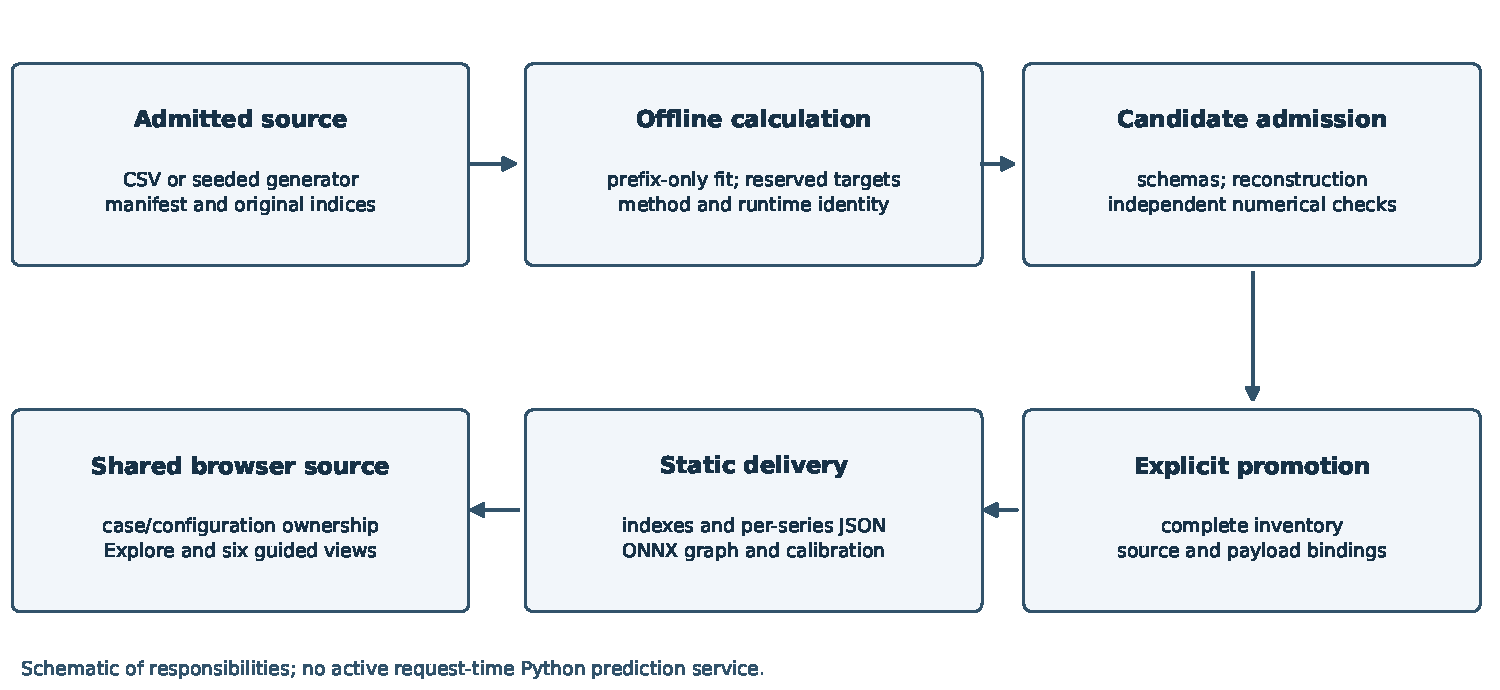
\includegraphics[width=\textwidth]{architecture.pdf}
\caption{Offline calculation, candidate admission, explicit promotion and static browser delivery form separate evidence boundaries; the diagram describes the implemented data flow rather than a request-time forecasting service.}\label{fig:report-architecture}
\end{figure}

The first stage resolves a case identity to its manifest, source description and preprocessing policy. For committed real excerpts, the input is the exact admitted CSV. For a generated mechanism, the case definition and seed determine the observations. Reconstruction checks the original length, the retained display samples and the reserved targets before permitting a comparison. A display trace can be sufficient to draw a picture while being insufficient to reconstruct the fitting series. The second stage supplies the contiguous prefix to the chosen adapter, applying any recorded context cap. Its output contains point and interval columns with the requested horizon. Fitting failures, unavailable dependencies and malformed outputs remain failures or explicit unavailable records; they are not filled by a different algorithm under the requested method name.

The third stage joins forecasts with targets and a historical seasonal scale. It computes scores at the method--case or method--origin level before aggregating at the study's declared unit. This distinction matters: averaging overlapping origins as if they were independent observations would change both the estimand and its uncertainty. The fourth stage constructs delivery documents and compact indexes. Large external-combination records are split by source series, while the complete compressed numerical archive retains the detailed historical selection calculation. The browser index is a navigation aid rather than a replacement for that archive. Independent admission rederives targets, scales, scores and combined paths before a candidate can replace the served documents.

The fifth stage is browser ownership. A single source provider owns the URL-selected case or generator configuration. It fetches the corresponding manifest and required artifacts, rejects subject mismatches, and discards obsolete asynchronous completions. Explore and the six guided views consume this same source. A remembered combination origin may be shown alongside a forecast only when its complete contiguous prefix, length, horizon and targets match; the prefix binding hashes little-endian float64 values. A coincident case name or equal sample count does not satisfy this condition. Generated histories use local computation, and the embedded ONNX path additionally verifies its graph and calibration metadata. These are distinct execution modes, stated in the interface.

Algorithm~\ref{alg:artifact-admission} describes admission as a refusal-oriented sequence. It does not retrain an archived model or certify its scientific accuracy. The existing process also binds stage inputs and payload fingerprints so that a partial case inventory cannot acquire the identity of a complete release. A candidate directory is built and checked before promotion; creating it does not silently overwrite the published data root. This ordering permits independent inspection of a concrete candidate and preserves evidence of a failed attempt.

\begin{algorithm}[htbp]
\caption{Admit a complete forecast artifact candidate against its declared source and execution identities before explicit promotion.}
\label{alg:artifact-admission}
\begin{algorithmic}[1]
\Require Declared case inventory, exact source inputs, implementation bindings, candidate artifacts
\State Refuse missing, extra or duplicated case identities
\For{each declared case}
  \State Validate manifest, trace and analysis against their normative schemas
  \State Reconstruct the complete contiguous source and verify retained samples and targets
  \State Verify the recorded producer and input bindings without rewriting historical identities
  \For{each required forecast path}
    \State Check horizon, finite values, ordered interval columns and method identity
    \State Recompute scores using the declared targets and historical scale
    \State Refuse disagreement beyond the recorded numerical tolerance
  \EndFor
  \State Verify optional study links against the complete prefix and target binding
\EndFor
\State Check index references, expected inventory and candidate payload fingerprints
\State Report an admitted candidate; retain explicit promotion as a separate operation
\end{algorithmic}
\end{algorithm}

This architecture supports independent numerical checks without making every browser request repeat model training. It also creates a responsibility to distinguish a stored result from a new execution. The archived-path comparison reuses some historical predictions, the fresh comparison executes the full roster again, and the external combination study has its own inputs and aggregation. Their schemas, provenance and consumer labels retain these distinctions. A successful schema check cannot substitute for a source reconstruction, and a successful reconstruction cannot establish representative sampling or pretraining independence. The report's evidence claims remain attached to the relevant stage rather than inherited from successful delivery.


\section{Implementation identities}
The method roster distinguishes algorithms from their implementations. A reference library, a direct adaptation and a small browser-exported model can share an architectural idea while differing in objectives, preprocessing and training budget. Their results remain separate.

\begin{longtable}{>{\raggedright\arraybackslash}p{0.22\textwidth}>{\raggedright\arraybackslash}p{0.32\textwidth}>{\raggedright\arraybackslash}p{0.37\textwidth}}
\caption{Forecasting implementations and their roles in the archived common-holdout comparison; a reference package, direct adaptation and browser demonstration retain distinct execution identities.}\label{tab:implementation-identities}\\
\toprule Methods & Implementation and settings & Evidence in the archived comparison\\\midrule\endfirsthead
\toprule Methods & Implementation and settings & Evidence in the archived comparison\\\midrule\endhead
SeasonalNaive, SES, Holt, HoltWinters, Theta & NumPy core; browser TypeScript parity; finite smoothing grids & Recomputed on original contiguous prefixes. Gaussian residual intervals are approximations.\\
AutoETS, AutoTheta, AutoARIMA & statsforecast; ARIMA stepwise and approximate, context cap 360 & Released paths rescored. Separate worked lessons freshly execute the installed adapters.\\
LightGBM & MLForecast lag table; 100 trees, 31 leaves, learning rate 0.05, context cap 500 & Released point-regression path rescored; Gaussian residual intervals. A lesson freshly executes the adapter.\\
NLinear, DLinear, NHITS & Direct-torch quantile-head adaptations & Released paths rescored; not asserted to be exact replications of the papers.\\
NLinear (nf), DLinear (nf), NHITS (nf) & neuralforecast reference implementations; fixed 300-step training budget & Released paths rescored; the budget is part of the experiment.\\
Chronos-Bolt, Chronos-2, TimesFM 2.5, TiRex-2 & Pretrained checkpoint adapters; TiRex bridge uses WSL/CUDA & Released paths rescored, without current-checkpoint or pretraining-independence claims.\\
ContextMemory, RecencyMean, EqualMean & Same five light experts; fixed causal memory and two ablations & Newly computed with matching original prefixes and final targets.\\\bottomrule
\end{longtable}

Table~\ref{tab:implementation-identities} identifies the archived comparison's implementations. The later complete fresh execution is reported separately, so a reader can distinguish rescoring an old path from executing its producer again.

The additional browser model is a separately identified normalized linear map, exported to ONNX after one global least-squares fit on generated windows. It predicts twelve observations from a forty-eight-observation prefix and is not the per-prefix NeuralForecast NLinear configuration in the twenty-two-variant experiment. Its frozen point matrix is preserved. A separate ridge-selection experiment did not improve point error; that candidate remains an experimental reference, not a replacement for the served graph.

The working browser implementation uses the independently evaluated prefix-stratified calibration described later in this report, rather than the old Gaussian scale in the legacy metadata. The calibration binds the exact graph digest, normalization, supported dimensions, roughness boundaries and finite-sample residual ranks. The browser refuses unsupported horizons, nonfinite or constant lookbacks, a changed model graph and malformed outputs. It does not silently truncate a requested longer horizon. Marginal calibration evidence comes from generated series; successful model execution on an authentic history does not establish coverage on that history's population.

\subsection{Corrected lightweight methods}
SeasonalNaive repeats the latest observed cycle. SES updates a level, Holt adds a trend, and additive HoltWinters additionally updates a seasonal component. At a prefix length $n$, the seasonal slot for zero-based future lead $k$ must continue as $(n+k)\bmod m$. Restarting at $k\bmod m$ is incorrect when $n$ is not a multiple of $m$. An adversarial partial-season example tests this condition independently in Python; the browser parity fixture includes a non-multiple history and a horizon longer than one cycle.

For the nonseasonal Theta implementation, the corrected point equation is
\begin{equation}
\widehat y_{n+h}=\ell_n+\frac{b}{2}\left[h-1+\frac{1-(1-\alpha)^n}{\alpha}\right],\qquad h\geq1,
\end{equation}
where $\ell_n$ is the selected SES level and $b$ is the fitted linear slope. An independent two-Theta-line construction verifies the finite-history term following Hyndman and Billah~\cite{theta}. This local method does not inherit AutoTheta's automatic seasonal adjustment merely because the names are related.

The Gaussian widening rule maps a residual standard deviation to three ordered columns at probabilities 0.1, 0.5 and 0.9. Residual estimation, Gaussian shape and horizon widening are assumptions. Neither an ordered matrix nor a quantile-loss fit establishes marginal or conditional calibration. These distinctions also apply to the direct neural adaptations and the lag-tree adapter.

\section{Forecasting equations and execution policies}
\label{sec:forecast-methods}

The following descriptions identify the fitted computation, its observation units and its actual execution policy. A library's ability to update a latent state does not mean the current adapter exercises that ability. All outer targets remain reserved; prefix caps, parameter search and numerical postprocessing belong to the compared configuration. Reference package versions and checkpoint revisions are retained with the corresponding experiment rather than inferred from a method's display name.

\subsection{Seasonal continuation and local smoothing experts}
\label{sec:method-local-experts}
The five local experts share a finite observed prefix and a requested observation-count horizon. They supply the matching inputs to the fixed and temporally selected combinations, and the browser implements the same point equations for generated examples. This parity does not imply that every browser score equals an offline score when the supplied history or scale differs. The pipeline first requires the experiment's admitted sequence. Interpreting decimated samples as consecutive observations would change the model, even if its implementation passed an arithmetic fixture.

SeasonalNaive continues the last observed seasonal cycle. With one-based lead $j$ and a zero-based sequence index, the future seasonal phase is $(n+j-1)\bmod m$. It therefore remains correct when the prefix ends partway through a cycle. The computational work for the point path is linear in the requested horizon after the relevant tail has been identified. Residual dispersion comes from observed lag-$m$ differences. A Gaussian interval constructed from those differences is an uncertainty approximation, not a distribution-free property of seasonal copying.

Simple exponential smoothing keeps a level and minimizes the implemented in-prefix one-step squared error over its fixed coefficient grid. With level $\ell_t$ and observation $y_t$, its update and point forecast are
\begin{equation}\label{eq:report-ses}
\ell_t=\alpha y_t+(1-\alpha)\ell_{t-1},\qquad \widehat y_{n+j}=\ell_n.
\end{equation}
The initial level is the first observation. The coefficient grid runs from .05 to .95 in increments of .05, with deterministic first-minimum selection. This is a finite search, not a claim of global continuous-parameter optimality. For a fixed grid its fitting cost grows linearly with prefix length. The level has source unit $U$ and the coefficient is dimensionless. Residual variance and final interval width still depend on how well a level-only description represents the supplied sequence.

Holt introduces an additive trend $b_t$ with units $U$ per observation. Its equations are
\begin{align}\label{eq:report-holt}
\ell_t&=\alpha y_t+(1-\alpha)(\ell_{t-1}+b_{t-1}),\\
b_t&=\beta(\ell_t-\ell_{t-1})+(1-\beta)b_{t-1},\qquad
\widehat y_{n+j}=\ell_n+j b_n.
\end{align}
The initial trend is the first observed difference. The implementation searches nine level coefficients from .1 to .9 and six trend coefficients from .05 to .5. It does not use a damped trend or select an arbitrary damping parameter. Extrapolation can therefore continue a recent trend too far after a break. Fitting every coefficient pair on the same prefix makes the finite objective reproducible but cannot ensure that its in-prefix preference remains appropriate for the reserved block.

Additive HoltWinters adds seasonal offsets $s_t$ in source units~\cite{fpp}. The implemented component updates are
\begin{align}\label{eq:report-hw}
\ell_t&=\alpha(y_t-s_{t-m})+(1-\alpha)(\ell_{t-1}+b_{t-1}),\\
b_t&=\beta(\ell_t-\ell_{t-1})+(1-\beta)b_{t-1},\\
s_t&=\gamma(y_t-\ell_t)+(1-\gamma)s_{t-m}.
\end{align}
The first cycle initializes level and offsets; the first two cycle means initialize trend. Four level coefficients, two trend coefficients and three seasonal coefficients form the fixed search. The residual objective begins after the first cycle, and a short or nonseasonal history falls back to Holt. A particular seasonal lag is supplied, not inferred by this expert. A wrong lag can therefore harm both the forecast and its residual-based interval.

The finite-history Theta equation given earlier uses the selected SES level and a fitted linear slope~\cite{theta}. Its correction term matters on short prefixes; replacing it by an arbitrary half-drift continuation changes the method. The five experts retain Gaussian residual endpoints on the specified probability grid. Ordered endpoints follow the implemented construction, while calibration remains an empirical question. Degenerate residuals, finite parameter grids and positive affine unit changes deserve explicit checks. These local experts provide transparent baselines and combination components; they do not establish that a short observed series admits an identifiable trend, stable seasonality or a calibrated future distribution.

For a fixed seasonal lag, evaluating a single SES or Holt coefficient tuple takes one pass through the prefix and a linear pass through the requested horizon. HoltWinters additionally retains one cycle of seasonal state. The finite coefficient grids multiply this cost by their recorded candidate counts; they are not continuous optimizers. Forecasting with an incorrect seasonal lag, a near-zero residual scale or an abrupt trend reversal can still fail despite an exact implementation. In particular, a zero residual history is not evidence that all future observations are known. The interval approximation and the point recurrence must therefore be evaluated separately, and a numerical parity fixture cannot establish distributional correctness.

\subsection{Automatic ARIMA, exponential smoothing and Theta selection}
\label{sec:method-automatic-statistical}
The automatic statistical adapter calls StatsForecast's AutoARIMA, AutoETS and AutoTheta implementations~\cite{statsforecast}. These are separate methods from the local finite-grid experts. The package owns its candidate models, optimization and interval construction. Passing the same seasonal count does not make the local Theta equation an equivalent implementation of AutoTheta, nor does an automatic label establish that every plausible forecasting model was searched. The published forecasting literature supplies the model families and selection motivation; the installed package and experiment records define the executed configuration~\cite{autoarima,etsstate}.

A seasonal ARIMA family can be expressed using a backshift operator $B$ as
\begin{equation}\label{eq:report-arima}
\phi(B)\Phi(B^m)(1-B)^d(1-B^m)^D y_t
=c+\theta(B)\Theta(B^m)\epsilon_t.
\end{equation}
Here $d,D$ are differencing orders, lower- and upper-case polynomials describe ordinary and seasonal autoregressive or moving-average terms, and innovations $\epsilon_t$ have source units. Model identification, stationarity constraints, root locations and innovation assumptions matter to forecasts and intervals. Differencing removes specified low-frequency components; it is not proof that the transformed future process will remain stationary. An estimated linear stochastic model also does not inherit coverage guarantees when its innovation distribution or stability assumptions fail.

The current AutoARIMA adapter requests stepwise search and approximate selection calculations. It caps the supplied history at the final 360 observations and uses a smaller historical backtest-window budget than the cheaper automatic methods. Those settings bound its cost; they can also alter its fitted result. A stepwise search is not exhaustive minimization over all order tuples. The common final-block experiment aligns reserved outcomes, but does not erase the context-cap difference or convert historical rolling aggregates with different origin counts into a common experimental budget.

Exponential smoothing can be written as an innovations state-space family. An additive level-and-trend member illustrates its form:
\begin{align}\label{eq:report-ets-state}
y_t&=\ell_{t-1}+b_{t-1}+\epsilon_t,\\
\ell_t&=\ell_{t-1}+b_{t-1}+\alpha\epsilon_t,\qquad
b_t=b_{t-1}+\beta\epsilon_t.
\end{align}
AutoETS selects among the package's admissible error, trend and seasonal structures; the equations above do not assert that every case selected this particular additive member. Multiplicative structures have additional positivity and distributional implications. The package's available model family and numerical fit determine whether a candidate is admissible. Automated selection can be useful when manual specification across many series is impractical, while remaining sensitive to sample size, initialization, objective choice and a structural break near the forecast origin.

For all three methods, the adapter fits a new model on each supplied prefix. It obtains the library's central point output from its mean field. For the canonical .1 and .9 columns it requests the corresponding central eighty-percent band. Calling the central output a median quantile would require assumptions beyond the field name; the report treats it as the package point forecast placed in the central column. The final cumulative maximum enforces column order. That repair is numerical postprocessing, not evidence that the columns equal the true conditional quantiles of an unknown data-generating process.

The library may support efficient state updates in other applications, but the evaluated adapter's interface uses a new fit and predict call. Its timings therefore cannot establish the performance of a native online state-update service. Computational work includes candidate search and parameter optimization as well as the recurrence associated with the selected model. JIT initialization, cached code, hardware and process policy can affect recorded latency. The shared targets and independently rescored paths support the finite accuracy comparison; they do not supply resource-normalized superiority, exhaustive search optimality or a universal forecast ranking.

Reproduction should record the supplied observations and the package version rather than attempting to infer an automatic configuration from its displayed score. A finite point path can survive an optimization warning; the warning is retained so the reader can distinguish a returned forecast from evidence of a well-converged fit. Conversely, a failed fit cannot become a successful experiment by copying another method's output. Short prefixes, multiplicative positivity restrictions and a seasonal period large relative to history are specific stress cases. The current selected-case result does not quantify how frequently these conditions occur in an operational population. Those frequencies and the cost of refitting at each arrival would have to be measured in a separate deployment study.

\subsection{Recursive lag-tree regression and approximate intervals}
\label{sec:method-lag-trees}
The lag-tree adapter uses LightGBM through MLForecast to fit a point regressor to one observed series~\cite{lightgbm,mlforecast}. The transformation is explicit: earlier values become input columns and the current observed value becomes the training target. It does not use the final reserved outcomes during fitting. The adapter constructs integer observation indices rather than genuine calendar features, and declares no static regressors. Consequently, its label should not imply that holidays, promotions, weather or future exogenous variables were supplied merely because the surrounding application can discuss those factors.

Let $\mathcal L$ be the selected lag set. The fitted one-step mapping and recursive multi-step use can be represented as
\begin{equation}\label{eq:report-lag-map}
\widehat y_t=F_\theta((y_{t-\ell})_{\ell\in\mathcal L}),\qquad
\widehat y_{n+j}=F_\theta((\widetilde y_{n+j-\ell})_{\ell\in\mathcal L}),
\end{equation}
where $\widetilde y_t$ is an observed prefix value when $t\le n$ and a previously generated prediction otherwise. This definition makes the origin's information boundary clear. It also exposes error propagation: after the first lead, some inputs are model outputs, not newly observed truth. An unusually accurate one-step fit does not establish stability of that recursion over a longer horizon or under a regime not represented in the supplied prefix.

The candidate lags begin with one, two and three. When the seasonal period is at least two, the candidates also include $m$, $m+1$ and $2m$. Duplicates are removed, and lags too close to the available prefix length are excluded using the implemented training-row allowance. The context cap is five hundred observations. Thus the number of retained lag columns and usable rows can differ across cases. A seasonal lag is a count of observations, while the lag values and regression target have the same source unit $U$. This adapter does not estimate a new seasonal frequency from the reserved targets.

The configured regressor has one hundred trees, at most thirty-one leaves, a learning rate of .05, a minimum child sample count of five and one worker thread. A generic squared-error boosting description is
\begin{equation}\label{eq:report-boosting}
F_T(x)=F_0(x)+\eta\sum_{r=1}^{T}f_r(x),\qquad \eta=.05,\quad T=100.
\end{equation}
Each fitted tree approximates an improvement to the current loss under the package's split and regularization policy. The LightGBM paper describes efficient implementation techniques, but this application does not separately reproduce the paper's speed comparisons or assert that every optional optimization is enabled. Fixing a tree count is a computational budget, not proof that the fitted function reached a global minimum or that a more expensive fit would improve the held-out criterion.

MLForecast is asked to retain fitted values. The adapter computes the population standard deviation of its in-sample one-step residuals, then applies the shared Gaussian horizon-widening rule around the recursive point path. Those residuals have already participated in fitting. Their dispersion can therefore be optimistic as an estimate of future uncertainty, and the recursive multi-step error distribution need not have the same shape. No native quantile-objective models are fitted by this adapter. The separate browser calibration experiment does not calibrate these tree intervals or alter their source identity.

A prediction call traverses the fitted trees at each future lead; a useful descriptive bound is proportional to horizon, tree count and visited tree depth. Training additionally depends on available rows, bins, feature count and the split search. The result is not constant-time forecasting in the observed history. The complete comparison retains both point and interval scores so that an apparent point improvement cannot conceal poor uncertainty quality. A faithful future change could evaluate direct quantile objectives or a separately calibrated residual procedure, but it would require its own method identity and held-out evaluation rather than rewriting the outcomes of this configured regression model.

The regressor's interval is consequently a separate approximation layered on a deterministic recursive mapping. Its training residuals are fitted residuals rather than errors from a held-out calibration sample, and their empirical scale may be optimistic. Heteroscedasticity, a changing level or accumulating recursive error can invalidate a common Gaussian shape even when its endpoints remain ordered. Increasing the number of trees would change the point model but would not by itself repair this uncertainty construction. A fair extension would compare a declared residual-calibration or quantile procedure on an untouched future block, retaining its information cutoff, resource budget and source units. That extension has not been substituted for the admitted tree result.

\subsection{Quantile-head neural adaptations and reference implementations}
\label{sec:method-neural}
The neural roster distinguishes three direct PyTorch adaptations from three NeuralForecast implementations. The source papers motivate NLinear, DLinear and N-HiTS~\cite{zeng,challu}; the package supplies its maintained model classes~\cite{neuralforecast}. Matching a name does not prove matching architecture, optimization, preprocessing or training budget. The report therefore retains the direct and library paths as separate experiment identities. Neither a favorable direct adaptation nor an unfavorable short-budget library fit is a replication of every result in the original paper.

The direct adapter standardizes its supplied observed prefix using the prefix mean $\mu$ and population standard deviation $s$. For $s>0$, the normalized sequence and inverse transform are
\begin{equation}\label{eq:report-neural-scale}
z_t=(y_t-\mu)/s,\qquad \widehat y=\mu+s\widehat z.
\end{equation}
Only prefix observations enter those quantities. The implementation uses a unit denominator when the standard deviation is exactly zero; that is a numerical fallback, not an empirically calibrated uncertainty model for constant series. It must not be confused with the browser linear consumer, which refuses a constant required lookback. Sliding training inputs and their future blocks are drawn entirely inside the supplied prefix. The final reserved outer block is not a training window.

A direct NLinear head subtracts the last value of each input window, applies one affine map and adds that value back to every lead and quantile:
\begin{equation}\label{eq:report-nlinear}
\widehat Z=\operatorname{reshape}_{H\times |Q|}\{W(x-x_L\mathbf1)+b\}+x_L.
\end{equation}
The output dimension is horizon times probability count, rather than the original single point path. DLinear instead forms a moving-average trend and a remainder, applies one affine map to each and sums their outputs. Its moving-average kernel is at most twenty-five and is adjusted to an available odd length; replicated edge padding remains inside the input window. The branch called seasonal in the implementation is the remainder after this moving average. It is not an estimated physical seasonal component with guaranteed period $m$.

The direct method labelled NHITS is a compact multi-rate MLP adaptation. It pools the input at rates four, two and one, sends each pooled vector through two hidden layers of width 128 with ReLU activations, and sums their horizon-by-quantile outputs. Its forward computation does not contain the full paper's hierarchical interpolation or an explicit residual-backcast chain. Accordingly, the description treats it as a separately documented adaptation, not a faithful reproduction of that architecture. This distinction also explains why the maintained library variant remains an independent comparator.

All three direct adaptations minimize the implemented multi-quantile pinball objective,
\begin{equation}\label{eq:report-neural-pinball}
\mathcal L(\theta)=\frac{1}{B H |Q|}\sum_{i=1}^{B}\sum_{j=1}^{H}\sum_{q\in Q}
\max\{q e_{ijq},(q-1)e_{ijq}\},\qquad e_{ijq}=z_{ij}-\widehat z_{ijq}.
\end{equation}
The supplied probabilities are .1, .5 and .9. The direct optimizer is Adam with learning rate .001 and a three-hundred-step budget. Each minibatch draws at most sixty-four training windows with replacement using a local seeded generator. Initial model weights are seeded separately through PyTorch. Those settings define the fit; they do not guarantee a global optimum, training convergence or bitwise equality across devices and library versions. The lookback prefers the larger of twice the horizon and three seasonal periods, capped to leave the required in-prefix training allowance. An insufficient lookback is an error rather than an invented fit.

The reference adapter instantiates NeuralForecast's corresponding classes with its multi-quantile loss, the declared input length, seed and three-hundred-step budget. It uses artificial hourly timestamps to supply regular index spacing, not real calendar semantics. GPU selection depends on the recorded runtime; CPU fallback is a distinct execution environment. The adapter resolves the package's output-column naming conventions for each requested probability and fails if a column cannot be identified. It then applies the same nondecreasing column repair used by other adapters:
\begin{equation}\label{eq:report-quantile-repair}
\widetilde q_j^{(r)}=\max_{a\le r}\widehat q_j^{(a)}.
\end{equation}
This cumulative maximum can change a central or upper column when raw heads cross. It preserves order but is not an isotonic least-squares projection and does not prove probabilistic calibration. The separate browser ONNX map has a global generated-window least-squares training identity and an independently studied residual calibration; it is neither one of these per-prefix neural fits nor a replacement for their empirical interval results.

Computational cost depends on the implementation as well as the architecture name. The direct affine models have parameter counts proportional to input length times horizon times the number of probability heads; the pooled MLP adaptation adds hidden-layer products at each pooling rate. Training multiplies per-minibatch work by the fixed three-hundred-step budget. The maintained library can use different internal batching and device policies. None of these finite budgets constitutes a convergence certificate. Reporting them makes a repeated experiment interpretable and avoids attributing a budget-specific failure to an entire model family.

\subsection{Pretrained checkpoint adapters and their information limits}
\label{sec:method-pretrained}
The pretrained roster contains Chronos-Bolt, Chronos-2, TimesFM 2.5 and TiRex-2. The local adapters load existing checkpoints and request forecasts; they do not fine-tune those weights on each selected case. Primary model descriptions explain the originating model families, while repository APIs and exact checkpoint revisions identify the executed variants~\cite{chronospaper,chronos,timesfmpaper,timesfm,tirex}. A paper about an earlier family does not by itself establish the architecture, licence or numerical identity of a later checkpoint. The admitted runtime records therefore retain checkpoint provenance separately from the human-readable method name.

At an outer origin, the adapter supplies a capped contiguous suffix of the observed prefix. A schematic description is
\begin{equation}\label{eq:report-checkpoint-map}
\widehat Q=\mathcal M_{\theta^*}(y_{n-C+1:n};H,Q),\qquad C\le n,
\end{equation}
where $\theta^*$ is a retained pretrained parameter set, $H$ is the requested horizon and $Q$ is the canonical probability grid. The prefix cap is part of the configuration. The expression is an interface definition, not an assertion that every checkpoint uses the same normalization, distribution head or internal computation. A common reserved block can align evaluation outcomes while the models consume different context lengths and possess very different external training histories.

Transformer-family attention is commonly represented as
\begin{equation}\label{eq:report-attention}
\operatorname{Attention}(Q_a,K_a,V_a)=\operatorname{softmax}(Q_aK_a^\top/\sqrt d)V_a.
\end{equation}
Here the subscript distinguishes attention matrices from the forecast probability set, and $d$ is an internal feature dimension. This equation describes a model component, not every operation in the Chronos or TimesFM checkpoint. Original Chronos uses scaling, quantization and language-model training; later family APIs and output heads must be identified separately~\cite{chronospaper,chronos}. TimesFM's originating description uses a patched decoder, while the evaluated 2.5 release has its own package interface and continuous quantile head~\cite{timesfmpaper,timesfm}. The report does not transplant benchmark scores from those papers into the selected ChronoScope cases.

TiRex-2 instead uses a recurrent xLSTM-based design~\cite{tirex}. Its originating paper reports streaming and multivariate capabilities, including covariate handling. Those capabilities must not be denied merely because the present adapter evaluates a univariate prefix interface. Conversely, loading that checkpoint for a full-prefix forecast does not mean this experiment exercised or timed its native incremental state update. The separate historical ACI/PID-style replay is also not a test of TiRex-2's streaming architecture. The mathematical distinction between a recurrent state and an external repeated-fit wrapper remains essential to interpreting the app's method names and timing plots.

The Chronos adapter maps requested quantile outputs from the package's supported tensor forms into a horizon-by-probability matrix. The TimesFM adapter maps the evaluated deciles to the corresponding output columns; the canonical .1, .5 and .9 requests are exact deciles. General non-decile behavior is not established by this experiment. The TiRex adapter explicitly rejects unsupported probability levels. A common final cumulative maximum enforces nondecreasing columns where applicable. None of these shape or ordering operations establishes that reported marginal probabilities are calibrated on the selected sources.

Checkpoint loading is cached within the relevant process so repeated windows can reuse a model. That cache changes loading cost, not the observations available at an origin. A timing comparison would need to distinguish cold loading, warm inference, process bridges, host memory and device transfers. The WSL/CUDA path for TiRex is an execution policy and cannot be treated as equivalent hardware to a native CPU call without measurement. The complete fresh comparison records package, checkpoint and source identities, but it is still a finite collection with one reserved block per selected series. Undocumented pretraining overlap, domain shift, training-corpus differences and configuration-specific context limits remain unresolved. The observed ranking therefore describes the admitted paths and targets; it does not certify universal zero-shot superiority or operational suitability.

For authentic sources, a further concern is information that entered the checkpoint before this experiment began. Hashing the input prefix proves the local inference input and cannot prove that the source was absent from pretraining. Likewise, a permissive software licence does not determine the terms of every weight release. The report retains the admitted checkpoint identity and its evaluated interface instead of silently upgrading to a newer family member. Any replacement would require new licence and configuration review, fresh matched-target execution and new evidence bindings before its score could replace the current result.




\section{A fixed context-memory proposal}
\label{sec:method-combinations}
ContextMemory tests whether similar completed historical contexts help estimate expert competence beyond recency alone. Feature-dependent combinations and dynamic ensembles are established ideas~\cite{fforma,ade}. The experiment tests a specific within-series recurrence rule and makes no priority claim for contextual weighting.

The expert set is fixed to SeasonalNaive, SES, Holt, HoltWinters and Theta. Up to twelve completed historical origins are selected within the prefix. For every origin $o$, eligibility requires $o+H\leq n$. A normalized half-window mean contrast, level shift, volatility-change statistic and seasonal correlation describe the context. Expert multi-step absolute losses are normalized using information available at that origin. A Gaussian context-distance kernel combines with recency weights of half-life six origins. Local estimated losses are shrunk 25\% toward the recency-only loss estimate.

An exponential loss transformation produces a simplex allocation, followed by a 5\% uniform floor. With $K=5$ experts, each final weight is at least $0.05/K=0.01$ and the weights sum to one. Corresponding point and quantile columns are averaged with these same weights. Nonnegative convex weights preserve the order of the input quantile columns. They do not make the result a calibrated predictive mixture.

RecencyMean removes context similarity while retaining the experts, historical origins, recency weighting and competence transformation. EqualMean assigns a uniform allocation. These matching ablations distinguish the contextual component from the more general benefit of combining methods. A positive scale and location transformation supplies a structural check away from numerical degeneracy thresholds. Completed-target eligibility and quantile ordering have independent adversarial tests.

The fixed-allocation means in Figure~\ref{fig:fixed-combination-means} retain the original contextual rule and both matching controls; their ordering does not establish a benefit from the added kernel.

\begin{figure}[htbp]\centering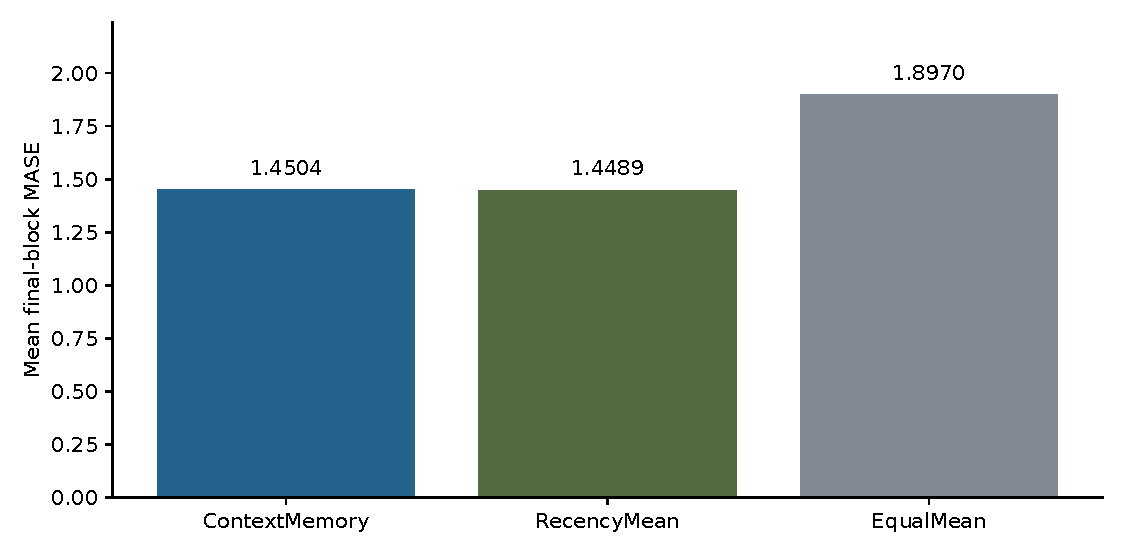
\includegraphics[width=0.87\textwidth]{proposal-comparison.pdf}
\caption{Fixed matching-expert combinations on the corrected fifteen-case protocol. Lower mean MASE is preferable. The contextual component does not improve on the recency-only ablation. Bars summarize selected final blocks, not independent population replications.}\label{fig:fixed-combination-means}\end{figure}


This section gives a complete mathematical interpretation of the implemented selection procedure. The proposal is the finite configuration tested in this paper, not a new general principle of stacking. Its input is one contiguous observed prefix, a positive seasonal lag and a positive forecast horizon. Its output includes three quantile columns, an expert allocation, the selected configuration, historical origins and validation records. There is no argument through which the caller can supply the outer reserved targets. Rejecting invalid or nonfinite input is part of the computation, rather than a reason to omit a difficult case after seeing its score.

\subsection{Three distinct information boundaries}
Write $\mathcal F_q=\sigma(y_1,\ldots,y_q)$ for the information supplied by the series through query $q$. The memory grid $\mathcal O_n$ is fixed from the length of the outer prefix and the declared lag and horizon. A validation query $v\in\mathcal O_n$ may use only the completed subset
\begin{equation}\label{eq:completed-set}
\mathcal T_v=\{o\in\mathcal O_n:o+H\le v\}.
\end{equation}
The rule requires at least three members before scoring that query. The validation origin's own context is computed from its prefix; its expert forecasts are computed from that same prefix. Historical loss rows and normalized signed errors used to fit its candidate weights come only from $\mathcal T_v$. The candidate's validation outcome is then formed from the block after $v$. That block is a target at this inner stage, although it is already observed at the final outer origin $n$.

Consequently, the whole inner validation calculation is available when the outer fit is issued. Provided the expert implementations are deterministic functions of their supplied prefixes and fixed configuration, the final weights are $\mathcal F_n$-measurable. This is an information-order statement. It does not assert that historical targets are statistically independent of their prefixes or of each other. Nor does it assert that a chronological split makes a changing process stationary. It simply specifies which observations can participate in each role and rules out use of the outer reserved block in fitting or selection.

There is a subtle limitation to the grid that must remain explicit. The origin grid is constructed from the supplied outer-prefix length. We then filter that grid at each historical query; we do not claim to recreate a historical service that would have selected its own independent grid knowing only its then-current length. The selected errors are chronologically available, but their sampling schedule is an offline evaluation design. A deployment requiring exact historical service reconstruction should issue and retain each prediction prospectively instead of interpreting this capped grid as such a log.

\subsection{Candidate scores and deterministic selection}
Let $\mathcal V_n$ be the validation queries with at least three completed training blocks. For a candidate $c$, let $w^{(c,v)}$ be its allocation fitted using those blocks, and let $E_{vhk}$ be expert $k$'s signed error at query $v$, lead $h$, divided by the query-prefix training scale. The recorded criterion is
\begin{equation}\label{eq:nested-score}
S_n(c)=\frac{1}{|\mathcal V_n|}\sum_{v\in\mathcal V_n}
\frac{1}{H}\sum_{h=1}^{H}\left|\sum_{k=1}^{K}E_{vhk}w^{(c,v)}_k\right|.
\end{equation}
Every candidate is scored on the same eligible queries. The selected configuration is the first configured minimizer of this criterion. Selection is then followed by a new weight fit using every completed memory block in the outer prefix. Historical validation estimates the performance of the allocation rule; its particular inner coefficient vector is not copied as if it were necessarily the correct final vector.

If no validation query qualifies, there is no historical selection estimate to minimize. The implementation records unavailable candidate means and explicitly selects the original recency-only candidate. That fallback can still allocate weights from any completed outer memory that exists. If the memory itself is empty, the allocation is uniform. Distinguishing these two cases matters: absence of an eligible validation split is not identical to absence of historical expert losses. Neither case justifies inventing a favorable validation score or replacing the fallback with the best outer-test method.

For a contextual candidate, let $g_k$ and $\ell_k$ be recency-weighted and context-and-recency-weighted normalized losses. Its shrinkage $\rho$ and temperature $\tau$ determine
\begin{equation}\label{eq:candidate-competence}
c_k=(1-\rho)\ell_k+\rho g_k,\qquad
v_k=\frac{\exp\{\operatorname{clip}[-(c_k-\min_jc_j)/\tau,-700,0]\}}
{\sum_l\exp\{\operatorname{clip}[-(c_l-\min_jc_j)/\tau,-700,0]\}}.
\end{equation}
Subtracting the minimum does not change exact softmax ratios and ensures that at least one unnormalized term is one. Clipping bounds numerical underflow in the remaining terms. Temperature changes concentration; shrinkage changes which loss estimate is concentrated. At $\rho=1$, the context distance has no effect. Thus selecting a configuration whose name belongs to the contextual family is not evidence that its kernel contributed to prediction quality.

\subsection{Regularized stacking on a simplex}
For stacking, arrange all completed training errors into a matrix $A$ with $N_e=JH$ rows and $K=5$ columns. Let $u=\mathbf1/K$ and $G=A^\top A/N_e$. The unfloored objective can be written
\begin{equation}\label{eq:quadratic-stacking}
F(w)=w^\top G w+\lambda(w-u)^\top(w-u),\qquad
w\in\Delta_K=\{w\ge0:\mathbf1^\top w=1\}.
\end{equation}
The Gram term preserves correlations and relative signs of expert errors. A candidate can therefore benefit from cancellation even when no single expert has uniformly small absolute loss. The penalty trades that fitted cancellation against proximity to equal allocation. Its fixed positive grid is part of the evaluated algorithm. Changing the penalty grid, expert set, memory schedule or error normalization produces another configuration, even if the public method label were left unchanged.

Because $G$ is positive semidefinite and $\lambda>0$, the Hessian is
\begin{equation}\label{eq:positive-hessian}
\nabla^2F=2(G+\lambda I)\succeq2\lambda I.
\end{equation}
The objective is strictly convex, and the nonempty compact simplex supplies a unique exact minimizer. This follows from standard convex optimization~\cite{boyd}; it is not a new statistical generalization theorem. Strict convexity does not imply good future forecasts, well-estimated covariances or correct interval coverage. It gives a well-defined fitting problem whose numerical answer can be checked independently of those empirical questions.

Five columns make exhaustive face enumeration practical. For a nonempty active set $B$, define $M_B=G_{BB}+\lambda I$, $x=M_B^{-1}\lambda u_B$ and $z=M_B^{-1}\mathbf1$. The equality-constrained stationary point on that face is
\begin{equation}\label{eq:face-solution}
w_B=x+\frac{1-\mathbf1^\top x}{\mathbf1^\top z}z,\qquad w_{B^c}=0.
\end{equation}
Positive definiteness makes the denominator positive in exact arithmetic. The implementation solves the two right-hand sides together, rather than explicitly forming an inverse. A face with a coefficient below $-10^{-10}$ or a nonfinite answer is rejected. Accepted coefficients are clipped only within the stated numerical feasibility tolerance and normalized before evaluating the original objective. All 31 nonempty faces are considered, including single-expert vertices, and a feasible equal allocation initializes the objective comparison.

Any simplex minimizer has a nonempty support. Its restriction to the relative interior of that support satisfies the corresponding equality-constrained first-order condition, while a boundary optimum appears on a smaller enumerated face. Therefore evaluating all feasible face solutions recovers the exact constrained optimum under exact arithmetic. In floating-point execution, tolerances and linear-system failures remain numerical concerns. Retaining feasibility, objective and independent reference checks is more informative than treating the absence of an iterative optimizer as an automatic certificate of numerical correctness.

The common uniform floor is applied after fitting:
\begin{equation}\label{eq:postfit-floor}
\widetilde w=.95w+.05u.
\end{equation}
The final allocation lies inside the simplex and each expert receives at least .01. It generally does not minimize $F$; the objective was solved for $w$, not for its floored transform. Likewise, the candidate is selected by scaled absolute validation error, not by $F$. These are two separate layers: a squared-error regularized fitting rule within a candidate and an absolute-error historical selection rule across candidates. Reporting both prevents the word optimal from obscuring which optimization was actually performed.

\subsection{What convex allocation guarantees}
At a fixed observation, convexity of absolute value yields
\begin{equation}\label{eq:jensen-error}
\left|y-\sum_kw_kp_k\right|\le\sum_kw_k|y-p_k|.
\end{equation}
The right side is a weighted average of component losses. It is not their minimum, and the inequality does not establish that the combination beats the best expert. The error may still be larger than that of an individual method or an equal average. Averaging over a horizon preserves the inequality for fixed weights, but does not turn historical weight estimation into an oracle for future errors. This limited consequence is useful for interpreting the algorithm without promising an empirical ranking.

For the same reason, positive expert weights preserve the order of already ordered quantile columns, but do not make their weighted columns a calibrated predictive distribution. Our experts' Gaussian residual approximations can be too wide, asymmetric relative to actual errors, or poorly adapted to horizon-specific uncertainty. A weight rule selected for absolute point error has no direct objective encouraging nominal marginal coverage. The observed high coverage and poor MSIS of several combinations are therefore substantive evidence about this construction, rather than a contradiction of convexity.

Finally, normalized features and errors explain why the allocation aims to be stable under a positive affine unit conversion. Away from degeneracy thresholds, translating the series cancels from mean contrasts and errors, while multiplication by a positive scale cancels from the corresponding standard deviations and seasonal error denominators. The expert equations must also transform consistently. The implemented absolute tolerances and finite precision require explicit exceptions near zero scales; we do not infer universal unit invariance from symbolic cancellation alone. Final evaluation retains unavailable MASE for a seasonal scale at most $10^{-12}$ in source units instead of silently using the training fallback.

The mathematical properties above support deterministic, inspectable fitting. They do not supply the missing independent comparator experiments, prospective confirmation on a deployment population, or an isolated attribution of gains to context. Those remain empirical questions. Complete validation records and retained adverse comparisons make the next experiment more precise: one can change a single allocation ingredient, preserve its information contract, and evaluate whether the previously observed point gains survive without reusing the new target block for selection.

\subsection{Computational and memory requirements}
Let $K$ be the expert count, $J$ the number of remembered origins, $V\le J$ the eligible inner-query count, $d=4$ the context dimension, and $Q=3$ the retained quantile count. Write $F_k(n_o,H)$ for the actual fitting and forecasting work of expert $k$ at prefix length $n_o$. Building the memory requires $\sum_{o\in\mathcal O_n}\sum_{k=1}^K F_k(n_o,H)$, in addition to context extraction and array construction. For the finite smoothing grids used here, the recursive fits are linear in prefix length with a fixed grid-size multiplier. They are fresh finite-prefix fits, not constant-time native state updates. The final expert paths require another fit on the complete supplied prefix.

Memory stores context rows, expert losses, normalized error rows and all historical quantile paths. Its numerical-array requirement is $O(Jd+JK+JHK+JKHQ)$, dominated by the historical paths when $H$ grows. The local LRU cache retains at most sixteen memory entries; their history-tuple keys also retain observed values. Cache reuse avoids repeating identical calculations but does not turn those values into newly observed information. Each worker has its own process-local cache, so increasing worker count can increase peak memory.

For one contextual candidate and inner query, distance and competence allocation cost $O(Jd+JK)$ after memory construction. Stacking first forms a $K$-by-$K$ Gram matrix from $JH$ error rows, costing $O(JHK^2)$. Enumerating every nonempty active expert set then has the upper bound $O(2^K K^3)$ for dense face solves. With $C_c$ non-stacking and $C_s$ stacking candidates, an upper bound for the inner allocation work is
\begin{equation}
 O\!\left[C_cV(Jd+JK)+C_sV(JHK^2+2^KK^3)\right],
\end{equation}
plus scoring the $H$-lead paths and the final selected allocation. In this experiment $K=5$, $J\le12$, $C_c=11$ and $C_s=4$; the exhaustive solver considers 31 faces. These fixed small values explain why exact face enumeration is feasible here. The exponential dependence on $K$ precludes inferring scalability to a large expert library from this experiment. We report no recovered hardware-normalized latency comparison: retained per-series seconds do not identify the historical machine or the elapsed makespan of parallel execution.


Algorithm~\ref{alg:fixed-combination} specifies the fixed context rule
and its controls. Algorithm~\ref{alg:report-temporal-selection} specifies
the completed-target selection used by the separately validated variants.
The outer reserved targets never enter candidate fitting.

\begin{algorithm}[htbp]
\caption{Combine five current expert forecasts using fixed contextual, recency-only or uniform weights estimated from completed origins.}
\label{alg:fixed-combination}
\begin{algorithmic}[1]
\Require Observed prefix, horizon $H$, seasonal lag $m$, probabilities and weighting rule
\State Form up to 12 unique integer origins evenly spaced from $\max(2m,2H+8,24)$ to $n-H$
\State Use the empty roster if the last eligible origin precedes the first
\State Compute the roster's prefix features and seasonal-scaled expert losses
\State Initialize equal weights
\If{the roster is nonempty and the rule is ContextMemory or RecencyMean}
  \State Compute mean loss for each expert with a six-origin recency half-life
  \If{the rule is ContextMemory}
    \State Compute RMS query distances and set bandwidth to the larger of their median and .25
    \State Compute the local kernel-weighted loss with .25 shrinkage toward the recency mean
  \EndIf
  \State Convert scores to softmax weights at temperature one and mix with .05 uniform weight
\EndIf
\State Fit the five expert quantile paths on the current prefix
\State Return their weighted columns, the weights and the eligible origin roster
\end{algorithmic}
\end{algorithm}

\begin{algorithm}[htbp]
\caption{Temporally completed candidate selection. Every expert forecast and
validation target used to choose a combination is available before the current
reserved target block begins.}
\label{alg:report-temporal-selection}
\begin{algorithmic}[1]
\Require Observed prefix $y_{1:n}$, horizon $H$, fixed candidates $\mathcal C$
\State Construct the fixed historical origin schedule and cache expert paths
\For{each historical query origin $q$}
\State Retain earlier origins $o$ satisfying $o+H\leq q$
\State Use the query only when at least three completed origins are available
\For{each candidate $c\in\mathcal C$}
\State Fit its weights from the completed historical memories only
\State Score its combined path on the query block using the query's prefix scale
\EndFor
\EndFor
\State Select minimum mean validation loss; break ties by the fixed grid order
\State With no eligible query, use the explicitly defined recency-only fallback
\State Fit the selected rule's current weights from all completed prefix memories
\State Return the weighted current expert path without observing $y_{n+1:n+H}$
\end{algorithmic}
\end{algorithm}


\section{Experimental protocol and archived results}
\subsection{Historical training-case ranking}
\label{sec:training-case-ranking}
The offline training stage evaluates the classical roster on each supplied training case with the same rolling evaluator used for case scoring. It accumulates the case MASE for each available method, omits NaN values, and sorts ascending by the unrounded arithmetic mean. A method with no recorded score sorts last. Ties follow the declared roster order. The stored scores are rounded to five decimal places only after ranking, and the first method is recorded as the default. Each training case with a score contributes one term; longer cases do not automatically receive more weight. This historical artifact depends on the caller's choice of training cases. It makes no per-prefix selection and has no independent confirmation stage. It is separate from the discovery-trained forest in Section~\ref{sec:forecastability} and does not determine the method shown as best on a reserved case.

The aggregation takes one pass over the available case scores and sorts the fixed classical roster. Repeated rolling fits dominate its cost. When two methods have missing scores on different cases, their means can summarize different subsets; record both denominators before using the ranking in a new evaluation.

\subsection{Archived common final-block protocol}
Each selected series supplies one forecast origin and one final block. Fourteen heavy forecast paths remain frozen; five corrected lightweight methods and three combinations are newly computed. Every admitted path is scored on the same actual values and horizon within its case. Original rolling-backtest results remain archived. Their differing origin budgets, ranging from three to more than twenty-five windows, make a direct ranking of those aggregates confounded by the evaluation schedule.

Let $y_1,\ldots,y_n$ denote the contiguous prefix, $a_1,\ldots,a_H$ the final targets and $p_j$ a point prediction. The historical seasonal scale is
\begin{equation}
s_m=\frac{1}{n-m}\sum_{t=m+1}^{n}|y_t-y_{t-m}|,
\end{equation}
with the lag bounded to the available history. MAE is $H^{-1}\sum_j|a_j-p_j|$, RMSE is the square root of mean squared error, and MASE is MAE$/s_m$~\cite{mase}. A value below one compares a future error with a historical scale. It does not directly show that the method beat an independently scored SeasonalNaive path on the same future block. A zero scale produces an unavailable scaled metric rather than an invented denominator.

For lower and upper columns $l_j,u_j$, empirical coverage is $H^{-1}\sum_j\mathbf1\{l_j\leq a_j\leq u_j\}$ and width is $H^{-1}\sum_j(u_j-l_j)$. With nominal interval miscoverage $\alpha=0.2$, the interval score is
\begin{equation}
IS_j=(u_j-l_j)+\frac{2}{\alpha}(l_j-a_j)_++\frac{2}{\alpha}(a_j-u_j)_+.
\end{equation}
MSIS is its block mean divided by $s_m$. The artifact's WQL uses only $Q=\{0.1,0.5,0.9\}$:
\begin{equation}
\mathrm{WQL}_3=\frac{2\sum_{q\in Q}\sum_{j=1}^H\rho_q(a_j-\widehat y_j^{(q)})}{3\sum_{j=1}^H|a_j|},\quad
\rho_q(e)=\max(qe,(q-1)e).
\end{equation}
This is an average of three quantile losses, not a complete predictive-density evaluation. A zero absolute-target sum makes this normalized score unavailable. Proper-score theory motivates reporting probabilistic quality, while the finite quantile grid limits what is observed~\cite{scores}.

\subsection{Archived-path final-block results}
Table~\ref{tab:archived-results} scores every admitted method on the same fifteen reserved blocks, without giving longer histories more weight in the case mean.
\begin{longtable}{lrrr}
\caption{Corrected common final-block comparison. Means weight each selected case equally.}\\
\toprule Method & Cases & Mean MASE & Mean coverage\\\midrule\endhead
Chronos-Bolt & 15 & 1.0363 & 0.7563 \\
TimesFM-2.5 & 15 & 1.0633 & 0.8071 \\
TiRex-2 & 15 & 1.0809 & 0.7694 \\
Chronos-2 & 15 & 1.1555 & 0.6905 \\
DLinear & 15 & 1.1600 & 0.5595 \\
AutoARIMA & 15 & 1.2104 & 0.7813 \\
NLinear & 15 & 1.2298 & 0.4524 \\
NHITS (nf) & 15 & 1.2546 & 0.5079 \\
NHITS & 15 & 1.2898 & 0.4857 \\
LightGBM & 15 & 1.2983 & 0.5786 \\
SeasonalNaive & 15 & 1.4137 & 0.8702 \\
RecencyMean & 15 & 1.4489 & 0.8889 \\
ContextMemory & 15 & 1.4504 & 0.8944 \\
AutoTheta & 15 & 1.4964 & 0.7329 \\
HoltWinters & 15 & 1.6778 & 0.8639 \\
AutoETS & 15 & 1.6940 & 0.7639 \\
NLinear (nf) & 15 & 1.7547 & 0.1821 \\
EqualMean & 15 & 1.8970 & 0.8611 \\
SES & 15 & 1.9167 & 0.8274 \\
Theta & 15 & 1.9224 & 0.8274 \\
Holt & 15 & 3.9846 & 0.7302 \\
DLinear (nf) & 15 & 10.7385 & 0.4996 \\
\bottomrule
\end{longtable}


Chronos-Bolt has the smallest mean MASE in this selected, mixed-provenance comparison, followed by TimesFM 2.5 and TiRex-2. Their paths were not freshly refitted or regenerated for this experiment. No statistical significance, resource-normalized superiority or independence from pretraining data follows from that order. Method-specific training budgets and context limits remain part of the compared configurations.

Coverage exposes substantial differences that a point ranking conceals. Several neural paths have narrow intervals and low observed coverage. A broad interval can increase coverage at the expense of decision usefulness; coverage alone should not be optimized. Individual case outcomes and widths remain available in the artifact and workbench, including unfavorable neural and combination results.

Figure~\ref{fig:fixed-case-differences} retains both signs of the case-level difference, so favorable examples cannot replace the stated aggregate comparison.

\begin{figure}[htbp]\centering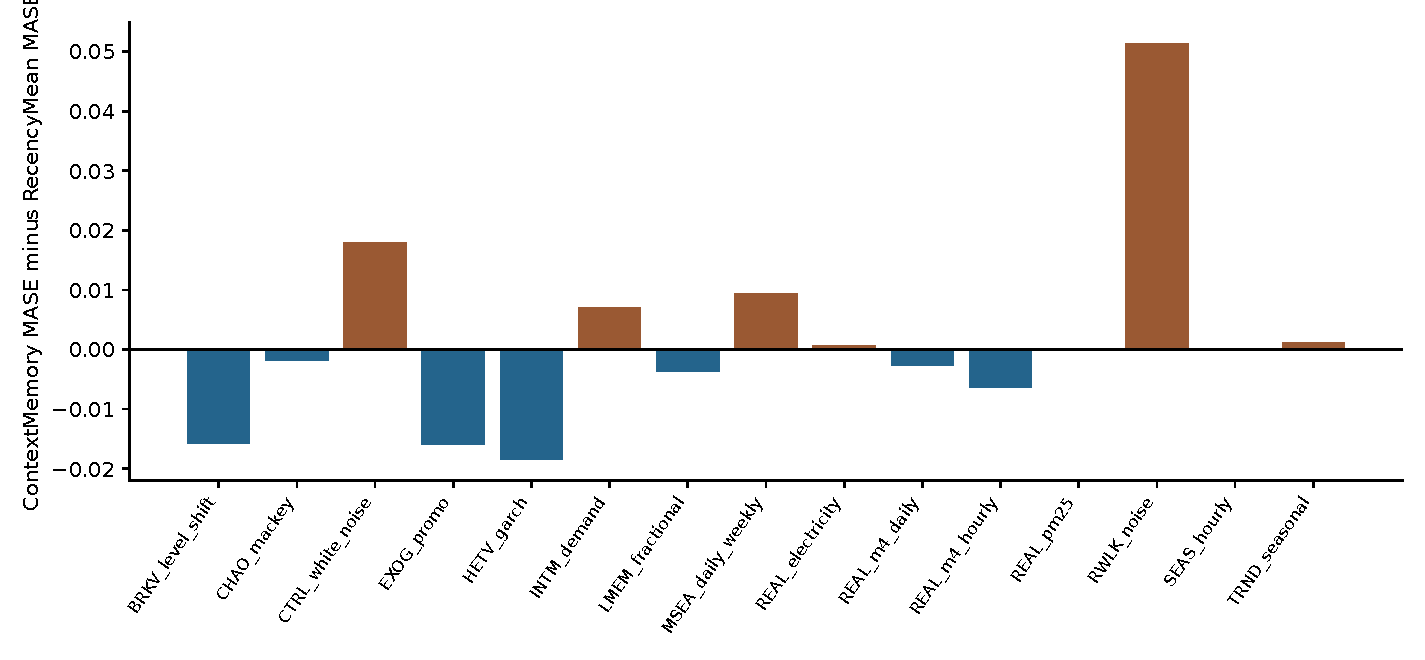
\includegraphics[width=\textwidth]{case-differences.pdf}
\caption{ContextMemory minus RecencyMean MASE for every selected case. Positive values favor the recency-only ablation. The common target and expert set isolate the contextual weighting component within each case, but the selected origins do not establish a general effect.}\label{fig:fixed-case-differences}\end{figure}

ContextMemory's mean MASE is 1.4504, versus 1.4489 for RecencyMean. The difference is unfavorable at the declared primary criterion, despite occasional individual improvements. EqualMean gives 1.8970. Settings are unchanged after either the invalidated display-history calculation or the corrected run. A changed configuration would define a new experiment and must not overwrite this result.


These summaries weight the selected cases equally rather than weighting every target value equally. A long horizon therefore does not acquire more influence merely because it supplies more scored leads. Conversely, an equal-case mean does not describe any known operational mixture of demand series. The reported average answers a question about this inventory, and changing the inventory could change its ordering. Per-case tables allow a reader to inspect that dependence instead of accepting the average as a universal ranking.

The archived-path result is also a comparison of recorded configurations, not a controlled assessment of architecture alone. Pretraining, context caps, optimization budgets and the distinction between an automatic reference implementation and a direct adaptation remain part of each method identity. No error bar over fifteen deliberately selected cases would remove these design differences. The separate external study supplies a larger and more explicitly accounted collection for its smaller roster; it does not retroactively turn this final-block exercise into a representative neural-model benchmark.

\section{Fresh execution of the complete roster}
A second experiment fits or infers all twenty-two configurations again from the same verified contiguous prefixes. The separately admitted artifact records every prediction, source-file and input hash, checkpoint revision, package version, fit/inference duration and warning category. An independent standard-library checker recomputes all seven metrics from the stored numerical arrays, verifies complete inventories and rejects trials, changed targets, frozen paths disguised as new fits and stale source bindings. These admission checks establish internal numerical consistency and recorded identity; they do not establish independence from model pretraining data.

The execution uses Python 3.12, NumPy 2.1.3, PyTorch 2.9.1 with CUDA 12.8, StatsForecast 2.0.3, LightGBM 4.6.0, MLForecast 1.0.31, NeuralForecast 3.1.9, Chronos forecasting 2.3.2, TimesFM 2.0.2 and TiRex-2 0.1.1. Its GPU is an NVIDIA GeForce RTX 4070 Laptop GPU. NumPy follows the TiRex-compatible line in this isolated Linux environment; notebook/parity computations use their separately pinned environment. Direct and reference neural models retain their declared 300-step budgets. LightGBM uses one worker; BLAS/OpenMP threads and compiler workers are bounded, and torch CPU operations use four threads. These resource choices are part of the recorded configuration.

Table~\ref{tab:fresh-results} pairs new executions with archived paths on the same outcomes; matching values describe recomputation rather than independent statistical replication.
\begin{longtable}{lrrr}
\caption{Fresh execution alongside the archived-path comparison. The same fifteen final blocks are used in both; these are not independent replications.}\\
\toprule Method & Archived MASE & Fresh MASE & Fresh coverage\\\midrule\endhead
Chronos-Bolt & 1.0363 & 1.0363 & 0.7563 \\
TimesFM-2.5 & 1.0633 & 1.0633 & 0.8071 \\
TiRex-2 & 1.0809 & 1.0809 & 0.7694 \\
Chronos-2 & 1.1555 & 1.1555 & 0.6905 \\
DLinear & 1.1600 & 1.1600 & 0.5595 \\
AutoARIMA & 1.2104 & 1.2104 & 0.7813 \\
NLinear & 1.2298 & 1.2298 & 0.4524 \\
LightGBM & 1.2983 & 1.2983 & 0.5786 \\
NHITS (nf) & 1.2546 & 1.2993 & 0.4968 \\
NHITS & 1.2898 & 1.3031 & 0.4746 \\
SeasonalNaive & 1.4137 & 1.4137 & 0.8702 \\
RecencyMean & 1.4489 & 1.4489 & 0.8889 \\
ContextMemory & 1.4504 & 1.4504 & 0.8944 \\
AutoTheta & 1.4964 & 1.4964 & 0.7329 \\
HoltWinters & 1.6778 & 1.6778 & 0.8639 \\
AutoETS & 1.6940 & 1.6940 & 0.7639 \\
NLinear (nf) & 1.7547 & 1.7547 & 0.1821 \\
EqualMean & 1.8970 & 1.8970 & 0.8611 \\
SES & 1.9167 & 1.9167 & 0.8274 \\
Theta & 1.9224 & 1.9224 & 0.8274 \\
Holt & 3.9846 & 3.9846 & 0.7302 \\
DLinear (nf) & 10.7385 & 10.7385 & 0.4996 \\
\bottomrule\end{longtable}


The two experiments use the same final targets, so rerunning an implementation is not another independent statistical test. Differences can reflect runtime, precision or training implementation rather than a changed data population. ContextMemory still fails its aggregate comparison with RecencyMean; the selected settings are not retuned after that outcome. Warning categories remain visible even when predictions are finite. Durations include fitting, inference, imports and first-use loading and cannot be interpreted as a normalized warm-inference leaderboard.

Exact Hugging Face revisions identify the four admitted pretrained checkpoints. The experiment retains its specified TimesFM 2.5 checkpoint and recorded licence. A newer upstream release would require separate review and execution rather than inheriting these results. This roster makes no claim to contain the latest released model of every family. The original streaming results below were not regenerated by this final-block execution.

Each admitted fresh path has the requested horizon and three ordered finite columns. Its execution record retains the package and checkpoint identities used for that run. A new successful run establishes computability for these inputs; it does not establish numerical identity across arbitrary devices or a new independent target realization.

\section{Comparison with four Timestral checkpoints}
\label{sec:timestral}
Timestral provides a pretrained multivariate quantile forecaster~\cite{timestral}. This experiment uses only its univariate interface. Every checkpoint receives the same complete observed prefix as the fresh common-block comparison, represented in float32. The input excludes the reserved target values. All 21 quantile columns are retained, with columns .1, .5 and .9 supplying the scored interval and center. The official CPU implementation uses four threads, symmetric averaging and nonnegative clipping under its model rules. Inference code, checkpoint revisions and the immutable reference digest were specified before Timestral execution, with the comparator outcomes already known.

Table~\ref{tab:timestral-scores} summarizes dimensionless scores across the same fifteen cases. They include four authentic excerpts and eleven generated cases. The raw MAE, RMSE and interval widths remain per case because the cases have different source units. Timestral-123M has the lowest observed mean MASE and MSIS within this set of four sizes. This ranking does not establish that another model-size ordering would hold across other data or that the smaller checkpoint dominates every case. The 209M checkpoint attains 89.14 percent mean case coverage in the four authentic excerpts and 73.86 percent across the generated cases. Those subgroup means illustrate why the aggregate coverage alone is insufficient.

\begin{table}[htbp]\centering\small
\caption{Case-weighted scores for four official Timestral checkpoints on the same fifteen reserved blocks, with a nominal 80 percent interval.}\label{tab:timestral-scores}
\begin{tabular}{lrrr}\toprule Checkpoint & MASE & MSIS & Coverage\\\midrule
Timestral-5M & 1.08491 & 4.80842 & 81.47\% \\
Timestral-28M & 1.05492 & 4.67321 & 81.94\% \\
Timestral-123M & 1.03585 & 4.61816 & 81.11\% \\
Timestral-209M & 1.04903 & 4.67244 & 77.94\% \\
\bottomrule\end{tabular}
\end{table}


The planned 209M minus AutoTheta mean case MASE difference is $-0.44740$. Twelve differences are negative and three positive. Ten thousand jointly reweighted case samples give a descriptive 95 percent percentile interval of $[-0.79356,-0.15991]$. These draws preserve the pairing but cannot establish population sampling independence. The baseline outcomes are from the unchanged fresh comparison, rather than concurrent benchmark execution on the same machine. Historical reference timing therefore cannot be used to infer a speed advantage from the recorded Timestral inference durations.

Two executions matched all 60 full quantile paths and case scores exactly on the recorded environment. Separate scoring logic verified the case errors, scores and directions against the held-out observations and recomputed the seeded reweighting interval. The complete numerical output records source, model and checkpoint-file hashes. The study does not resolve vendor pretraining overlap with the public sources. It supplies no estimate of benefits from multivariate or known-future covariates, and it does not reproduce the vendor's broad benchmark rankings. These limitations distinguish observed performance on the selected blocks from prospective use on unseen source populations.


The companion table \path{next/tables/fresh-by-case.csv} gives all twenty-two
fresh method scores on each of the fifteen final blocks. With one block per
case, the individual case scores are direct measurements on that block.
Repeated lead errors within a block do not provide independent replications.
A paired reweighting across selected cases measures sensitivity to their
relative weighting. It cannot supply within-case uncertainty over a future
forecast origin or a population confidence interval for a source collection.

\section{Combinations selected by temporal validation}
\label{sec:temporal-validation}
ContextMemoryCV and ValidationMix extend the fixed combination with parameter selection inside the observed prefix. They retain SeasonalNaive, SES, Holt, additive HoltWinters and finite-history Theta as experts. At a remembered validation origin $v$, a training block beginning at $o$ is eligible only if $o+H\le v$. At least three fully completed training blocks are required. Candidate scores average scaled absolute error over these causally held-out historical blocks. Without eligible validation, the method falls back to the original RecencyMean rule. No outer target is accepted by the fitting API.

ContextMemoryCV selects among context shrinkages $\{0,.5,1\}$ and temperatures $\{.15,.5,1\}$ plus the recency-only and equal-weight controls. ValidationMix additionally considers regularized convex stacking, minimizing mean squared normalized expert-combination error plus $\lambda\|w-\mathbf1/5\|_2^2$ over the simplex, for $\lambda\in\{.01,.1,1,10\}$. Five experts permit explicit active-set enumeration. A 5\% uniform floor is applied after fitting. Candidate ranking uses historical absolute error; the selected rule is refit on all completed memory blocks. All families and parameter values are fixed before the external outcomes are evaluated. Established stacking and temporal-validation principles are not claimed as new general ideas.

The external sources are complete Monash M4 Weekly and M3 Monthly inventories~\cite{m4weekly,m3monthly}. Horizons and seasonal periods are $(13,52)$ and $(18,12)$, respectively. Every method receives at most the final 512 contiguous observations at an origin. Up to three nonoverlapping final blocks are used, with a minimum available prefix of $\max(2m,2H+8,24)$. Sixty-five weekly identities have no eligible origin, leaving 294 series and 882 origins. Six exact duplicate monthly identities are excluded, leaving 1,422 series and 3,547 origins. Every source identity and exclusion remains available. Origins are averaged within series, then series equally within each collection. This is not the original forecasting-competition protocol or an official competition ranking.

Table~\ref{tab:validated-combinations} keeps point error, coverage and interval score together, making the collection-specific interval weaknesses visible alongside the point-error gains.
\begin{table}[htbp]\centering\small
\caption{Complete external comparison. W denotes 294 eligible M4 Weekly series; M denotes 1,422 unique M3 Monthly series. MASE and MSIS average origins within series and then series equally; Cov is empirical interval coverage. These are descriptive summaries, not confidence intervals.}\label{tab:validated-combinations}
\begin{tabular}{lrrrrrr}\toprule Method & W MASE & W MSIS & W Cov & M MASE & M MSIS & M Cov\\\midrule
SeasonalNaive & 0.8446 & 8.1670 & 0.9326 & 1.0864 & 8.8123 & 0.9342\\
SES & 0.3533 & 2.3404 & 0.8926 & 1.0456 & 7.1945 & 0.8534\\
Holt & 0.3806 & 2.4611 & 0.8844 & 1.8040 & 10.8472 & 0.8005\\
HoltWinters & 0.5396 & 3.0778 & 0.8413 & 0.9375 & 6.7112 & 0.9160\\
Theta & 0.3469 & 2.3237 & 0.9041 & 1.0021 & 7.0453 & 0.8700\\
AutoETS & 0.3413 & 1.8490 & 0.8713 & 0.8514 & 4.1518 & 0.7324\\
AutoTheta & 0.3076 & 1.7125 & 0.8511 & 0.8472 & 4.2994 & 0.7279\\
ContextMemory & 0.3079 & 2.9468 & 0.9751 & 0.9086 & 6.8846 & 0.9348\\
RecencyMean & 0.3109 & 2.9315 & 0.9742 & 0.9085 & 6.8846 & 0.9348\\
EqualMean & 0.3548 & 3.3233 & 0.9702 & 0.9962 & 7.2131 & 0.9333\\
ContextMemoryCV & 0.2848 & 2.5538 & 0.9511 & 0.8996 & 6.7999 & 0.9329\\
ValidationMix & 0.2855 & 2.5477 & 0.9503 & 0.8993 & 6.8208 & 0.9326\\
\bottomrule\end{tabular}\end{table}

Figure~\ref{fig:validated-combinations} compares the two external collection means with AutoTheta; the point-error ordering remains separate from the interval-score comparison.

\begin{figure}[htbp]\centering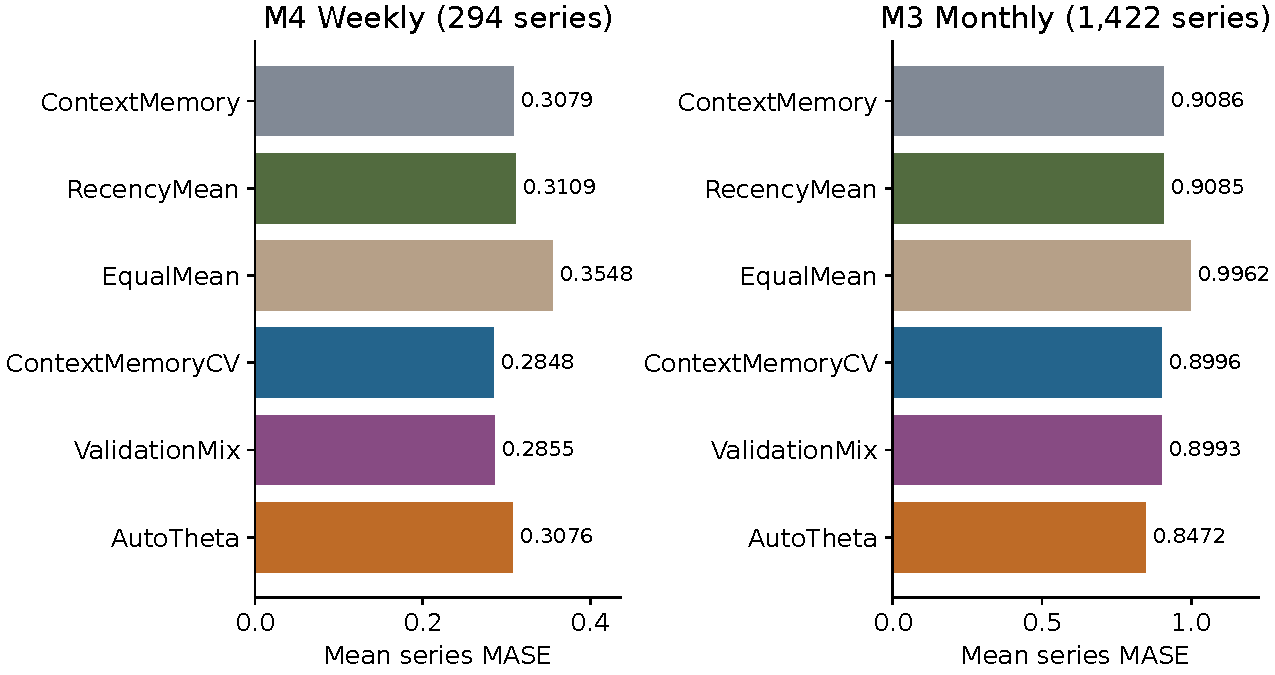
\includegraphics[width=.98\textwidth]{validated-combinations.pdf}
\caption{The new temporally selected combinations and fixed controls on each external collection, with AutoTheta as an automatic-statistical comparator. The complete twelve-method table retains the other individual experts and AutoETS. Bars are descriptive mean MASE without population confidence intervals.}\label{fig:validated-combinations}\end{figure}

ValidationMix lowers mean MASE relative to RecencyMean on both admitted collections, .2855 versus .3109 weekly and .8993 versus .9085 monthly. ContextMemoryCV gives .2848 and .8996. AutoTheta's .3076 weekly result is higher, while its .8472 monthly result is lower. The point improvement therefore depends on collection and comparator. Context shrinkage, temperature and temporal selection change together; this comparison does not isolate the causal value of the context kernel alone.

Interval quality remains unfavorable relative to AutoTheta. ValidationMix gives weekly MSIS 2.5477 and coverage .9503, and monthly MSIS 6.8208 and coverage .9326. AutoTheta gives 1.7125 and .8511 weekly, and 4.2994 and .7279 monthly. Nominal coverage is .8. These weighted Gaussian endpoints are not calibrated by minimizing point error, and wider intervals do not establish a better decision rule.

Table~\ref{tab:paired-main} reports a retrospective paired-series calculation on the retained forecasts. First average all admitted origins within each series and method. For each control, subtract its series loss from the corresponding ValidationMix loss. Resample the resulting paired differences with replacement within each collection, keeping the number of selected identities fixed at 294 or 1,422. Ten thousand draws use PCG64 with seed 20261105 plus the first four bytes of the SHA-256 of the collection identifier interpreted in little-endian order. The endpoints are the linear 2.5 and 97.5 percent quantiles of the resampled means. This operation does not refit an expert, choose a new parameter or treat the repeated origins as independent replications. The complete retained evidence includes 36 comparisons. The intervals were calculated after seeing the original results and remain exploratory and unadjusted for multiplicity or source dependence.
\begin{table}[htbp]\centering\small
\caption{ValidationMix minus each control after averaging available origins within each series. Unadjusted exploratory 95\% paired-series intervals describe the admitted collection, not population-wide superiority.}
\label{tab:paired-main}
\begin{tabular}{lllrrr}\toprule
Collection & Control & Loss & Difference & 95\% interval & Lower loss\\\midrule
Weekly & RecencyMean & MASE & $-0.025337$ & $[-0.033914,-0.017227]$ & 190/294\\
Monthly & RecencyMean & MASE & $-0.009154$ & $[-0.013176,-0.005173]$ & 589/1422\\
Weekly & AutoTheta & MASE & $-0.022065$ & $[-0.037521,-0.008272]$ & 155/294\\
Monthly & AutoTheta & MASE & $0.052154$ & $[0.032437,0.073112]$ & 689/1422\\
Weekly & RecencyMean & MSIS & $-0.383808$ & $[-0.431160,-0.334374]$ & 252/294\\
Monthly & RecencyMean & MSIS & $-0.063788$ & $[-0.088692,-0.040255]$ & 589/1422\\
Weekly & AutoTheta & MSIS & $0.835230$ & $[0.650853,1.038115]$ & 49/294\\
Monthly & AutoTheta & MSIS & $2.521379$ & $[2.364504,2.673453]$ & 267/1422\\
\bottomrule\end{tabular}\end{table}


The monthly mean MASE difference from RecencyMean is $-0.009154$, with an interval from $-0.013176$ to $-0.005173$. Only 589 of 1,422 monthly series have lower error than RecencyMean. These two statements describe the distribution of magnitudes and the frequency of improvement, respectively. Monthly AutoTheta still has lower point error, and its interval score remains lower in both collections. The positive ValidationMix minus AutoTheta MSIS differences in Table~\ref{tab:paired-main} quantify the cost of the point-selected mixture's interval construction under this scoring rule.

On the original fifteen development blocks, ContextMemoryCV and ValidationMix give mean MASE 1.3974 and 1.4031, while the original fixed ContextMemory and RecencyMean results remain 1.4504 and 1.4489. Their MSIS values, 9.5025 and 9.3428, are worse than RecencyMean's 9.1076. These already examined cases are not new external confirmation. The separate original twenty-two-variant execution and complete M4 Daily association/selection study remain unchanged.

All 53,148 method--origin forecast paths are independently rescored against their source-derived targets and seasonal scales. Final expert weights reconstruct the combined quantile paths. Temporal splits, complete historical targets, candidate losses and chosen parameters remain in the compressed numerical file. Browser delivery uses a compact index and separately fetched per-series documents, rather than downloading the entire numerical file for one chart. Every displayed path is independently checked against its stored score. Exact duplicates do not imply that all remaining series are independent or free of related-source overlap; no population or operational-superiority conclusion follows.

\section{Streaming evaluation as separate evidence}
\label{sec:streaming-evidence}
The historical streaming experiment uses a predict--observe--update order~\cite{dawid}, but the point forecaster is recomputed on each full observed prefix. Its artifact key \texttt{Theta} denotes a smoothing-plus-half-drift adaptation, not the corrected finite-history Theta equation used in the final-block comparison. ACI-style~\cite{aci} and PID-style controllers adapt the effective miscoverage level of a normalized-residual FIFO buffer. The PID-style rule is not a faithful implementation of published Conformal PID~\cite{pid}; its guarantees are not imported by name. No native stateful model update or framework capability comparison is evaluated.

A full numerical reconstruction exports 21,296 method-cutoff rows across fifteen cases, with targets, forecast endpoints, scores, buffer sizes and controller states. Every archived coverage trajectory and final weighted quantile loss matches at saved precision. At nominal 80\%, mean rolling absolute coverage error is .0830 for the raw smoothing-plus-drift base, .0656 for its ACI-style controller and .0645 for its PID-style controller. The much smaller .0416, .0057 and .0060 values measure absolute deviations after temporal averaging, which permits local errors to cancel. These are different statistics. Scaled widths and interval scores accompany coverage.

The reconstruction also varies coverage (.7, .8, .9), two point bases and three gain multipliers, retaining all 630 case-setting rows. Eleven generated mechanisms are repeated at two additional seeds, while the four real excerpts are not assigned artificial repetitions. These are sensitivity calculations on the same selected design, not independent population confirmation. The original gains have no recovered historical tuning rationale, and original per-call hardware metadata remain unavailable. Historical latencies therefore support no normalized runtime comparison. Exact source arrays and hashes permit numerical replay without claiming to restore missing acquisition history. These streaming outcomes are separate from both the final-block experiment and the M4 Daily corpus study.

The information order is observable at the row level. A prediction uses the current prefix and the residual buffer available before its target is revealed; only after scoring does that target affect the next fit and controller state. The record therefore supports a direct audit of a potential one-step timing error. Recomputing a prefix at each cutoff has a different computational cost from incrementally updating sufficient state. The former is the procedure reconstructed here, so no measured replay duration is transferred to a native online implementation. Buffer capacity, seasonal scaling and clipping also affect the resulting intervals and remain part of the controller configuration.

\subsection{Browser delivery and executable teaching artifacts}
Fifteen catalog boundaries cover traces, manifests, the index, diagnostic analysis, streaming results, ONNX metadata/assets, confirmed browser calibration, the retained ridge study, archived-path and fresh comparisons, historical selector metadata, the complete daily corpus study, the validated-combination index and its per-series records, and release readiness. Normative JSON Schemas validate the committed JSON documents. An OpenAPI component inventory generates browser TypeScript types without activating a prediction API. Cross-field invariants, source hashes, temporal reconstruction and numerical parity remain executable tests.

The browser delegates chart interaction, summaries, tables, reset controls and keyboard support to the pinned shared shell. The product supplies data adapters, stable method identities and scenario state. Bilingual content uses locale-aware numbers; model and licence versions retain their identity. Request cancellation and generation identifiers prevent a slower case request or inference result from overwriting a newer selection.

Numbered local workflows check prerequisites, initialize declared environments, build an external data candidate and start the development server. Generation binds source and payload fingerprints, refuses partial inventories and changed frozen inputs, and separates candidate creation from explicit promotion. Historical engine-version metadata is retained rather than relabeled to match the new browser release. An unused epidemic-model surrogate inherited from an older repository structure was removed.

Sixteen executed English and Spanish notebooks cover a seasonal reference, an incomplete-season experiment, actual statistical/tree adapter execution, the fixed combination with its ablations, sequence patterns, multiscale complexity and disjoint-series corpus inference. Their metadata records exact direct dependencies, sources, inputs and method coverage. Fresh-kernel execution and byte comparison check that committed outputs are current. Numerical convergence notices are retained as portable text; machine paths and incidental notebook metadata are excluded.

\section{Sequence diagnostics and corpus evaluation}
\label{sec:method-sequence}
\subsection{Diagnostic atlas and computational boundaries}
The diagnostic toolkit contains ten families: stationarity, autocorrelation, seasonality, filtering and decomposition, change points, volatility, distribution and complexity, fractals, nonlinear dynamics, and causality. Methods include ADF/KPSS and related tests, ACF/PACF and Ljung--Box diagnostics, STL/MSTL and periodograms, offline change-point procedures, ARCH/GARCH diagnostics and surrogate-based nonlinear analyses. A short series or unavailable dependency produces an explicit unavailable result for that analysis; it does not silently produce a substitute measurement.

Statistical diagnostics are descriptive or model-dependent. An autocorrelation band containing the observed coefficients does not prove white noise. A unit-root test does not certify future stationarity. A fractal estimate is sensitive to sample length, detrending and the assumed stochastic class. A nonlinear surrogate rejection does not uniquely identify deterministic chaos. The workbench exposes these cautions alongside the results rather than presenting a diagnostic label as a forecasting guarantee.

The browser recomputes lightweight diagnostics and light forecasts for generated scenarios. Committed analysis artifacts retain their original scope; several describe the complete observed series, including what later becomes a forecasting holdout. They are suitable for retrospective explanation, not for feature selection at the earlier forecast origin. The proposed combination computes its own prefix-only contexts and does not consume those retrospective diagnostics.

Heavy statistical, neural and pretrained calculations run offline. GPU availability, checkpoint caches and Python environments are distinct from the served browser bundle. A local environment with only NumPy cannot be represented as a complete neural or foundation-model rerun. Conversely, rescoring a stored model path does not require pretending that its original runtime has been restored.

The procedure crosswalk in \path{next/tables/procedure-crosswalk.csv} connects
each executable procedure to its method section, validation file and example
of retained evidence where available. It distinguishes callable diagnostics
from those with retained values. All fifteen archived bivariate panels have
a skipped marker, while current typed dispatch is exercised by runtime tests.
The shared dispatch conditions are described below, and each fitted
statistic retains its separate interpretation.

Algorithm~\ref{alg:diagnostic-dispatch} shows the shared availability and input
rules of the retrospective analysis stage. Its individual calculations are
specified in the following subsections. A reported panel error preserves
failure rather than inserting a zero-valued scientific result.

\begin{algorithm}[htbp]
\caption{Dispatch retrospective diagnostic panels on one admitted series}
\label{alg:diagnostic-dispatch}
\begin{algorithmic}[1]
\Require Observations $y$, declared period $m$, case identity, seed and typed covariates
\State Compute univariate panels on $y$, preserving exceptions as panel errors
\State Set $z\gets y$
\If{an admissible robust STL fit has seasonal strength at least $0.64$}
  \State Set $z\gets y-S$ using its seasonal component $S$
\EndIf
\State Compute break and regime diagnostics on $z$
\If{$y$ contains at least 400 observations}
  \State Derive a local case seed and run the nonlinear panel with nine surrogates
\Else
  \State Record an unavailable nonlinear panel
\EndIf
\If{a typed covariate has a complete aligned history}
  \State Compute the pair diagnostics using that first covariate
\Else
  \State Record unavailable pair diagnostics
\EndIf
\State Bind the original-axis sequence diagnostics to the full record
\State \Return diagnostic panels and availability records
\end{algorithmic}
\end{algorithm}

\subsection{Unit roots, stationarity and differencing}
\label{sec:diagnostic-stationarity}
The legacy univariate adapters remove nonfinite entries before fitting. A lag then refers to the compressed sequence, so a missing observation can change the temporal meaning of a lag. The sequence-extension adapters instead require a finite contiguous history. The analysis stage applies these diagnostics to the full available case record, which can include observations later reserved for forecast scoring. Its diagnostic results cannot be used as historical predictors without recomputing them inside the relevant prefix.

The augmented Dickey--Fuller regression~\cite{adf} is
\begin{equation}
 \Delta y_t=c+\gamma y_{t-1}+\sum_{j=1}^{p}\phi_j\Delta y_{t-j}+e_t .
\end{equation}
The adapter uses a constant and chooses augmentation order by AIC in Statsmodels 0.14.6. It tests the unit-root null using the statistic for $\gamma$, whose reference distribution differs from an ordinary regression $t$ test. Phillips--Perron keeps a constant and uses the \texttt{arch} 8.0.0 tau statistic with a long-run covariance correction. Its bandwidth controls the correction for serial dependence and is distinct from the augmentation order. DFGLS first removes the deterministic level using GLS detrending, then estimates a Dickey--Fuller regression on that residual sequence, with lag selection delegated to the pinned backend. The Zivot--Andrews call searches admissible interior breaks with the constant-break specification. Its selected break index maximizes evidence for the test's alternative under that specification. It does not identify a known external event.

KPSS reverses the direction of the null. For residuals from the level model, with $S_t=\sum_{i\le t}e_i$ and long-run variance estimate $\widehat\omega^2$, the statistic is
\begin{equation}
 K=\frac{\sum_{t=1}^{n}S_t^2}{n^2\widehat\omega^2}.
\end{equation}

For the Phillips--Perron calculation, regress $y_t$ on an intercept and
$y_{t-1}$ for the $N=n-1$ usable rows. Let $\widehat\rho$ be the lag
coefficient, $b$ its OLS standard error and $u_t$ the regression residual.
Compute $s^2=\sum u_t^2/(N-2)$ and $g_0=\sum u_t^2/N$. Let $L^2$ be the
Bartlett-weighted Newey--West long-run variance on the undemeaned residuals,
using $\lceil 12(n/100)^{1/4}\rceil$ lags. The backend's default tau statistic is
\begin{equation}
 Z_\tau=\frac{\sqrt{g_0}}{L}\frac{\widehat\rho-1}{b}
       -\frac{L^2-g_0}{2L}\frac{Nb}{s}.
\end{equation}
The backend converts this value with its constant-specification MacKinnon
reference. A zero coefficient standard error or too few residuals for the
bandwidth refuses the test. The long-run covariance sum costs $O(Nk)$ for $k$
included lags. DFGLS uses the constant-only local coefficient $1-7/n$ to
quasi-difference $y$ and the constant, preserving their first rows. It fits
the quasi-differenced level by least squares and subtracts that level from
the original observations. The final lag count minimizes AIC on the
OLS-demeaned series with no deterministic regressor, using the backend's
sample-size lag cap. Fit a no-intercept augmented regression to the
GLS-demeaned observations with that lag count and report its lagged-level
$t$ statistic using the DFGLS reference. Both wrappers clean the input
before fitting and retain the probability and decision at .05.

Zivot--Andrews uses the Statsmodels approximation that selects lags once.
Run ADF with constant and trend and choose the lag count by AIC, then
hold that count fixed for all break candidates. Discard the first and last
15 percent of the record from the candidate search using the backend's
integer trim. Fit the intercept-break regression at each remaining
position and retain the most negative lagged-level $t$ statistic. The
library looks up the associated probability for that break specification
and returns the zero-based minimizing index. This scan performs one
regression per eligible candidate. Rank failure in the auxiliary design
can leave the entire panel unavailable.
The Statsmodels adapter selects bandwidth automatically~\cite{kpss}. Probability values at the ends of its tables can be bounds. At level .05 the differencing routine checks KPSS repeatedly after applying $(1-B)$, where $B y_t=y_{t-1}$. It stops at two differences, fewer than eight values, a constant, nonrejection or a numerical exception. Thus its returned order is a recommendation and may encode an early stop. Seasonal differencing uses robust STL strength $\max(0,1-\mathrm{Var}(R)/\mathrm{Var}(S+R))$ and applies $(1-B^m)$ once if strength reaches .64. Short histories and zero denominators return zero strength. The serialized \texttt{stationary} flag means rejection of the unit-root null for ADF, Phillips--Perron, DFGLS and Zivot--Andrews. For KPSS it means nonrejection of level stationarity. The ADF/KPSS panel labels the two true flags stationary and the two false flags nonstationary. A true ADF flag with a false KPSS flag gives its difference-stationary label. A false ADF flag with a true KPSS flag gives its trend-stationary label. These disagreement labels are heuristics from the two level specifications. The test probability and reference critical values are dimensionless. Only the Zivot--Andrews result includes \texttt{break\_index}, a zero-based position in the cleaned sequence serialized as a number. Phillips--Perron and DFGLS use the pinned \texttt{arch} defaults for their bandwidth and lag choices. Zivot--Andrews uses the pinned Statsmodels defaults for its trim and AIC lag selection. A failed backend call can leave the stationarity panel unavailable.

\subsection{Correlation, periodicity and multi-seasonal decomposition}
\label{sec:diagnostic-autocorrelation}
The sample autocorrelation at lag $k$ divides the lagged centered cross-product by the centered sum of squares. Statsmodels computes it using its FFT branch at up to forty lags. The partial autocorrelation uses adjusted Levinson--Durbin recursion, so its coefficients describe the remaining association after intermediate lags enter the autoregression. The wrapper's $n-1$ cap alone cannot satisfy the backend's stricter short-sample PACF limit. Both displays compare nonzero lags to the same pointwise white-noise band $z_{1-\alpha/2}/\sqrt{n}$ at $\alpha=.05$. A significant-looking isolated lag in that display has not been corrected for selection across lags.

\begin{align}
 Q_{\mathrm{BP}} &= n\sum_{k=1}^{K} r_k^2,&
 Q_{\mathrm{LB}} &=n(n+2)\sum_{k=1}^{K}\frac{r_k^2}{n-k},\\
 D &=\frac{\sum_{t=2}^{n}(y_t-y_{t-1})^2}{\sum_{t=1}^{n}y_t^2}.
\end{align}
The panel uses Box--Pierce and Ljung--Box at $K=10$, with zero fitted-model degrees of freedom supplied to the backend. A chi-square approximation addresses the specified serial correlations. It cannot certify independence. The Durbin--Watson formula is evaluated on the cleaned levels in this panel. The familiar residual interpretation around two requires the conditions of a regression residual calculation. The separate lag-pair API returns $(y_{t-k},y_t)$ for $1\le k<n$, which can be inspected in source units for direct analysis. The baked panel omits these paired values.

Both correlograms store objects ordered by integer lag, including lag zero.
Their significant-lag lists exclude zero and contain the lags for which
the absolute coefficient strictly exceeds the common band. The portmanteau
probabilities are in $[0,1]$, with \texttt{white\_noise} true on nonrejection
at .05. For the stored \texttt{identification\_hint}, check Ljung--Box
first. The producer takes its white-noise-like branch when
\texttt{white\_noise} is true. When that flag is false and at least
four nonzero ACF lags are available,
average the absolute coefficients separately over the later half of
each nonzero-lag array. An above-band ACF tail and below-band PACF tail
suggests AR. The reverse suggests MA. Two above-band tails suggest
ARMA. Equality or two below-band tails give a mixed reading.
A nonfinite Ljung--Box probability also sets the flag false, so the
heuristic can emit the mixed reading on a constant series whose
probability serializes as null. A true test rejection requires a finite
probability below .05. The stage performs no model order search for
this field.

Algorithms~\ref{alg:unit-root-tests} and~\ref{alg:correlation-and-period}
give the test-specific branches and distinguish the two lagged analyses
from the spectral summaries.
\begin{algorithm}[htbp]
\caption{Compute the stationarity decisions and differencing recommendations from one finite cleaned series.}
\label{alg:unit-root-tests}
\begin{algorithmic}[1]
\Require Cleaned observations and an optional declared period
\State ADF: select the augmentation lag by AIC and test the lagged level in the augmented regression
\State KPSS: compute the partial-sum statistic with automatic long-run variance bandwidth
\State Phillips--Perron: fit the lagged-level regression and apply the Newey--West tau correction
\State DFGLS: quasi-difference the level design, choose lags on the OLS-demeaned series and fit the GLS variant
\State Zivot--Andrews: select one lag count, scan admissible breaks and keep the minimum statistic and index
\State Interpret the two null directions, then repeat KPSS with differences up to order two
\State When the period is eligible, evaluate robust STL strength for the seasonal recommendation
\end{algorithmic}
\end{algorithm}

\begin{algorithm}[htbp]
\caption{Compute lag statistics and period summaries on the cleaned observation axis using the declared defaults.}
\label{alg:correlation-and-period}
\begin{algorithmic}[1]
\Require Cleaned observations and declared candidate periods
\State Compute FFT ACF and adjusted Levinson--Durbin PACF through the admissible lag cap
\State Store coefficient rows, nonzero above-band lags, portmanteau results and the Durbin--Watson ratio
\State Evaluate the identification hint from the Ljung--Box flag and absolute tail averages
\State Compute one-sided periodogram and Welch densities and select each maximum nonzero-frequency bin
\State Fit robust STL to eligible candidate periods for strength and to the admitted rounded spectral period for the summary
\State Store complete periodogram bins, compact Welch and available decomposition strengths
\end{algorithmic}
\end{algorithm}

The SciPy 1.15.3 periodogram and Welch calls use one sample per observation step and choose the highest nonzero-frequency bin. A peak frequency $f$ gives period $1/f$ in observation steps. Welch averages windowed spectra over segments of length at most 256, reducing variance while coarsening frequency resolution. The winning bin can exist even on noise or a spectrum without meaningful positive power. The stage tests the declared period and twice that period for robust STL strength. For an admissible rounded spectral period, it computes $y_t=T_t+S_t+R_t$ and reports trend and seasonal strength ratios. At least two complete periods are required. The public MSTL adapter iteratively estimates multiple seasonal components, then exports their sum with the trend and remainder. A separate phase-subseries API reshapes complete cycles and reports phase means, discarding the final incomplete cycle. Neither of those two APIs is called by the default panel.

STL estimates the seasonal component by smoothing detrended observations
within each phase with local regressions, then removes a low-pass
component from the smoothed seasonal sequence. It smooths the
deseasonalized sequence for the trend and repeats these steps. The
single-period wrapper enables robust residual weighting. Statsmodels
0.14.6 supplies the smoothing windows and inner and outer iteration
defaults. The resulting trend, seasonal and residual arrays have source
units and share the cleaned observation axis in the direct API. The baked
\texttt{stl\_at\_dominant} object exists only when the periodogram peak
has period at least two and its rounded integer $p$ satisfies $p\ge2$
and $n\ge2p$. It stores the one-period list and dimensionless trend and
seasonal strengths in $[0,1]$. It omits the three component arrays.

The separate MSTL wrapper admits periods at least two and refuses a
cleaned record shorter than twice its largest period. The pinned
backend can remove a period at or beyond half the record length.
It sorts eligible periods, starts their components at zero, adds back
the old component for each period, applies STL to the partly
deseasonalized values, and subtracts the updated component before
advancing. It makes two sweeps for multiple periods and one for a
single retained period. The wrapper passes no power transform or custom
smoothing windows. It returns the sum of the seasonal columns on the
cleaned axis. Its period field lists the requested admissible input
periods. The cost grows with the number of period passes and the
underlying STL smoothing cost per pass.

The periodogram uses SciPy's one-sided density scaling, constant detrending and a boxcar window. For a non-edge positive bin $k$ on an $n$-sample record, its density is twice the squared magnitude of the discrete Fourier coefficient of the centered observations, divided by $f_s n$. The zero and Nyquist bins, when present, are not doubled. Frequencies are cycles per observation step, and the density is in $U^2/(\text{cycles per step})$ for source unit $U$. Multiplying by bin width before summation restores squared source units. The reported peak power has density units. The corresponding period is the reciprocal of peak frequency, in observation steps. Welch uses a Hann window and half-segment overlap under the pinned defaults. Its compact output retains peak power and period rather than the aligned frequency and density arrays. If no positive-frequency bin is available, the record contains \texttt{dominant\_period=null} and \texttt{dominant\_power=0.0}. A numerical failure produces an error record instead of a spectrum.

\subsection{Filters, intrinsic modes and wavelet energy}
\label{sec:diagnostic-filters}
The Hodrick--Prescott calculation estimates the trend vector $T$ by solving
\begin{equation}
 \min_T\sum_t(y_t-T_t)^2+1600\sum_{t=2}^{n-1}(T_{t+1}-2T_t+T_{t-1})^2 .
\end{equation}
The fitted trend and residual cycle share the source unit. The fixed penalty is not adapted to hourly or daily sampling. Baxter--King instead truncates a symmetric band-pass filter with periods 6 to 32 and 12 coefficients on either side. Its direct result drops 12 observations at each end. The default filter panel omits that result. The Christiano--Fitzgerald panel uses the same nominal band and a drift adjustment, with asymmetric endpoint weights from its random-walk approximation. Full-length output does not make this filter causal.

EMD sifts envelope means from extrema until the backend identifies an intrinsic mode, then repeats on the residue. The panel retains at most six modes and uses the EMD-signal 1.9.0 stopping rules. Its plain EMD seed argument has no effect. The separate CEEMDAN entry point uses 50 noise-assisted trials with a local noise seed, which controls the perturbations. The default filter panel runs plain EMD. The modes depend on the algorithm and do not identify physical sources by themselves. Continuous wavelet energy uses the Morlet wavelet on a fitted linear detrend. For 64 geometrically spaced periods from two to $\max(4,n/2)$ the scale is period times the wavelet's central frequency. PyWavelets 1.8.0 supplies the coefficients. The panel sums their squared magnitudes over time, retaining one energy per scale, while the direct method can return the full time-scale array. Edge effects and significance are not corrected. Wavelet fitting requires at least eight observations and shorter arrays are refused.

For CEEMDAN, standardize by the input standard deviation and decompose
the seeded normal noise realizations with EMD. Normalize each trial's
noise modes by the standard deviation of its first noise mode. Add
that first noise mode times .005 to the standardized record, extract
one mode per trial and average the first modes. At each later step, perturb the residual
with the corresponding noise mode scaled by $0.005$ times the residual
standard deviation when that mode is available. Apply a single-mode EMD
to each perturbed residual and average its local means. Subtract that
average from the current residual to obtain the next mode. The backend
stops when the residual fails to support another mode, its range is
below .01 or the sum of absolute residual values is below .05 on the
normalized scale. It appends the final residual as the last component
row, restores source scale and returns a separate reconstruction
closure residual. Work scales with the
number of trials and sift iterations per extracted mode. A degenerate
zero-variance input cannot be interpreted through this normalization.

The baked filter object stores the cleaned-axis HP trend and cycle and
the CF cycle in $U$. Its CF band contains the lower and upper periods
in observation steps. EMD modes form an array of rows, each containing
one value per cleaned observation. The residue follows the same axis.
For fewer than eight observations the direct CWT call raises an error,
whereas the panel omits \texttt{scalogram} if the earlier filters
succeed. An error from a filter that is invoked replaces the panel with
an error record. The retained scalogram aligns period and energy arrays,
stores the maximum-energy period and names the wavelet. Energy is a
sum of squared coefficients over the cleaned axis in squared source
units.

Algorithm~\ref{alg:filter-recipes} records the distinct filters and
the additional callable decomposition routes.
\begin{algorithm}[htbp]
\caption{Apply the filter, mode and wavelet procedures to the same cleaned input with separate output axes.}
\label{alg:filter-recipes}
\begin{algorithmic}[1]
\Require Cleaned observations $y$
\State HP: solve the penalized smooth-trend problem and subtract the trend
\State CF: apply the drift-adjusted asymmetric band and retain its full-axis cycle
\State BK when requested: use the symmetric finite band and return the shortened cycle
\State EMD: sift successive modes and return the remaining residue, capped at six modes for the panel
\State CEEMDAN when requested: decompose seeded noise and extract ensemble modes with adaptive residual scaling
\State CWT for $n\ge8$: detrend, transform at 64 Morlet scales and sum squared coefficients by scale
\State Emit the baked HP, CF, EMD and eligible CWT summaries
\end{algorithmic}
\end{algorithm}

\subsection{Breakpoints, latent regimes and volatility}
\label{sec:diagnostic-breaks}
When robust STL strength reaches .64, the stage subtracts the seasonal component before the change-point panel. If the decomposition fails, the original record enters the panel. PELT with the squared-error segment cost searches for
\begin{equation}
 \min_{\tau_1,\ldots,\tau_k}
 \sum_{j=0}^{k}\sum_{t=\tau_j}^{\tau_{j+1}-1}(y_t-\overline y_j)^2
 + k\,2\widehat\sigma^2\log(\max(n,2)).
\end{equation}
Here $\tau_0=0,\tau_{k+1}=n$, each segment has at least five observations, and the default variance proxy is half the population variance of first differences with a $10^{-8}$ fallback in squared source units. The \texttt{ruptures} 1.1.10 implementation prunes the search under its cost conditions~\cite{pelt} and evaluates interior candidates on a five-observation grid. The separately callable binary segmentation uses the same default grid and greedily splits with a supplied number of breaks. The terminal index $n$ is omitted from the exported breakpoints. Segment summaries use half-open zero-based bounds, with a mean and population standard deviation over each segment.

The CUSUM statistic is the maximum absolute scaled partial sum of residuals after removing the sample mean, using the OLS-residual reference test at .05. The two-state Markov regression estimates state-dependent means and variances and a transition matrix. Its plotted state path is the argmax of smoothed full-record probabilities. It can change retrospectively when observations arrive. The direct fit returns an $n\times 2$ array of smoothed state probabilities, one row per cleaned observation. The retained panel stores the argmax path, two fitted regime means in source units and a $2\times 2$ transition matrix. Rows identify destination regimes and columns identify origin regimes. The fitted switching variances and smoothed probabilities are absent from the retained summary. Five of the fifteen retained analysis panels contain a state path and ten contain a nested Markov error. A returned path does not certify optimizer convergence.

For volatility, ARCH-LM regresses squared demeaned values on twelve lagged squares and tests with the effective sample size times the auxiliary $R^2$. A rejection triggers a Gaussian constant-mean GARCH(1,1) fit with internal rescaling:
\begin{equation}
 \sigma_t^2=\omega+a e_{t-1}^2+b\sigma_{t-1}^2 .
\end{equation}
The panel retains parameters, $a+b$ and log likelihood, while the direct fit also provides conditional standard deviations. These estimates are in the backend's fitted scale when rescaling is applied. Rolling standard deviation uses sample degrees of freedom one and a trailing window $\min(20,\max(3,\lfloor n/10\rfloor))$, with leading nulls. The Box--Cox implementation adds $1-\min(y)$ when needed for positivity. For shifted positive $x$, the transform is $(x^\lambda-1)/\lambda$ or $\log x$ at $\lambda=0$. With a declared period of at least two, Guerrero estimates $\lambda$ from seasonal-subseries relative variability; without that period, the panel uses profile likelihood. The shift and selected exponent are needed to reverse the transformation. Its additive one is in source units and can change the result under unit conversion.

The volatility record's lag orders and rolling window count observations. The ARCH probability is dimensionless and lies in $[0,1]$. The rolling mean and standard deviation use the input units and align to the cleaned-series positions, with nulls before the first complete window. The fitted GARCH constant mean and variance intercept have units $U_{\rm fit}$ and $U_{\rm fit}^{2}$, respectively. The shock coefficient, variance coefficient and their sum are dimensionless. The log likelihood is in natural log units on the fitted scale. The serializer does not retain the backend's numerical rescaling multiplier, so the stored mean and intercept cannot by themselves be converted back into physical units. The lack of a GARCH result after an ARCH-LM nonrejection records a decision to skip that fit. It does not imply zero volatility.

The pinned Guerrero routine retains the last complete blocks of length
$m$. For each block $j$, compute its positive shifted mean $\mu_j$
and sample standard deviation $s_j$. Use bounded Brent search over
$[-0.9,2]$ to minimize the sample coefficient of variation of
$s_j/\mu_j^{1-\lambda}$ across those blocks. With at most two periods
of data the backend returns $\lambda=1$ directly. The block moments
take linear work in the retained record length. Each objective
evaluation then scales with the number of blocks. The wrapper passes
the selected exponent to SciPy for the transform. Without a declared
seasonal period of at least two, SciPy selects the exponent by its
profile likelihood instead. The separate log option fixes the exponent
at zero. The baked \texttt{boxcox} object holds only the method label,
dimensionless exponent, nonnegative input-unit shift and reference.
A failed transform produces a nested error in place of these fields.

Algorithm~\ref{alg:break-volatility} shows which decisions govern
the expensive fits and their output branches.
\begin{algorithm}[htbp]
\caption{Dispatch structural-break and volatility computations with their separate input transformations and eligibility decisions.}
\label{alg:break-volatility}
\begin{algorithmic}[1]
\Require Cleaned observations and a declared period when available
\State Use the robust-STL adjustment for break analysis when the strength gate is met
\State Run PELT on the selected break input, retaining segment bounds and statistics
\State Compute OLS-CUSUM and fit the two-state Markov model, preserving a nested fit error
\State On the unadjusted observations, compute ARCH-LM and trailing volatility
\State If ARCH-LM rejects, fit GARCH. Otherwise record its skip
\State Shift to a positive input and estimate Box--Cox by Guerrero or profile likelihood
\State Record transform failures and GARCH failures in their individual branches
\end{algorithmic}
\end{algorithm}

\subsection{Distribution, scaling and deterministic-dynamics diagnostics}
\label{sec:diagnostic-complexity}
The distribution panel computes a population standard deviation, biased sample skewness and excess kurtosis. Jarque--Bera evaluates $n(g_1^2/6+g_2^2/24)$ against its asymptotic reference. Shapiro--Wilk is run only from 3 to 5,000 observations. It evaluates the normal order-statistic pattern and neither test supplies serial-independence evidence. The baked \texttt{normal} flag requires Jarque--Bera nonrejection and, where available, Shapiro--Wilk nonrejection at .05. It retains both probabilities, with a null for unavailable Shapiro--Wilk, and omits the statistics returned by the direct summary. Kernel density uses SciPy Gaussian kernels at one hundred points spanning the sample, with bandwidth chosen by the library and density in inverse source units. A singular covariance can fail the panel even when the moments were computable. The normal Q--Q calculation returns ordered observations against theoretical standard-normal quantiles, with a fitted slope in source units.

The scalar entropy diagnostics use AntroPy 0.2.2. Sample entropy calls the default order two and tolerance .2 times population standard deviation, independently of the public ordinal pattern order. Permutation entropy uses order three, unit delay and normalization by $\log(3!)$. Welch spectral entropy divides the Shannon entropy of normalized spectral powers by the log of the bin count. These are distinct from multiscale sample entropy below. BDS compares an embedding correlation integral against the independent-product reference at dimension two, with the default radius 1.5 standard deviations and only for $n\ge20$. The direct complexity result carries the BDS statistic and probability. The panel keeps only \texttt{bds\_pvalue} and \texttt{iid}, with nulls for both when BDS is ineligible or fails. The flag means nonrejection at .05. Catch24 retains 22 backend-named features plus the original mean and standard deviation in source units. Each catch22 value has the interpretation of its keyed backend feature. If \texttt{pycatch22} cannot be imported, the record sets \texttt{available} to false and stores a reason and reference in place of the feature map.

R/S scaling fits the log rescaled range across observation scales. The first call uses the simplified random-walk estimator; on failure it uses the nolds polynomial fit. DFA estimates the slope of log root-mean-square fluctuation after linear detrending of integrated profiles. The panel maps a DFA slope above one by subtracting one, then averages the mapped value with R/S for its interpretation label. Values below .45 give the anti-persistent label, values above .55 give the persistent label and the inclusive middle gives the random-walk-like label. The \texttt{reliable} flag only indicates $n\ge100$. The distinct \texttt{arfima\_link.d} field is $H_{\mathrm{RS}}-1/2$ rounded to four decimal places. It is a descriptive proxy. For $n\ge200$, MF-DFA uses linear detrending on 24 geometrically spaced scales from 8 to $\max(16,\lfloor n/4\rfloor)$, truncated to integers and deduplicated, with $q$ in $\{-5,-3,-2,-1,1,2,3,5\}$. From slopes $h(q)$ it calculates $\tau(q)=qh(q)-1$, $\alpha(q)=\mathrm{d}\tau/\mathrm{d}q$ and $f(\alpha)=q\alpha-\tau(q)$. The panel stores aligned $q$, $h(q)$, $\alpha(q)$ and $f(\alpha)$ arrays and omits $\tau(q)$. Width above .15 is a heuristic flag. A short input or failed fit yields a nested error. A nonfinite value from a completed fit is represented by null at its array position. Higuchi uses graph lengths up to lag ten, Katz uses path length and extent, and Petrosian counts sign changes of first differences. Their empirical graph estimates do not identify an attractor dimension. The public DCCA coefficient normalizes the summed detrended profile covariance by the geometric mean of the two detrended variance sums at one scale. It uses $s=\max(8,\lfloor m/8\rfloor)$ by default on the shared length $m$ and linearly detrends the two integrated profiles within each of the $m-s$ overlapping windows of length $s+1$. It refuses $s\ge m$ and returns a nonfinite coefficient for a zero denominator. The implementation cleans the series separately before truncating to shared length, so callers must align missing observations before this call. The default panel omits this direct result.

The AntroPy 0.2.2 Higuchi calculation forms $k$ offset subsequences
for each $k=1,\ldots,10$. For offset $j$, let
$M=\lfloor(n-1-j)/k\rfloor$. It sums the $M$ absolute increments
at step $k$ and multiplies the sum by $(n-1)/(k^2M)$. Average the
normalized lengths across offsets and regress their logarithms on
$\log(1/k)$. This needs $O(nk_{\max})$ work for the lengths. A
constant path or offset with no increments can make the slope
unavailable. Katz uses $L=\sum_{t=2}^n|y_t-y_{t-1}|$,
$a=L/(n-1)$ and $d=\max_t|y_t-y_1|$. Its value is
$\log(L/a)/\log(d/a)$. Petrosian counts the sign-bit transitions
$Z$ in the first-difference array and evaluates
$\log n/[\log n+\log(n/(n+0.4Z))]$. Both take linear work in
the record length. The Katz calculation is undefined on a constant
path and can exceed two on finite samples.

Delay embedding forms $(y_t,y_{t+\ell},\ldots,y_{t+(d-1)\ell})$, requiring a nonempty vector roster. The canonical nonlinear panel uses $d=4$, $\ell=1$ and $n\ge400$. Correlation dimension estimates a slope of $\log C(r)$ against $\log r$, with $C(r)$ the fraction of close pairs. The Lyapunov adapter fits average log-neighbor divergence versus observation step, with temporal exclusion $\max(5,\lfloor n/200\rfloor)$. Both slope fits use seeded robust regression and a least-squares fallback. Recurrence quantification caps the embedding at 800 vectors, constructs Euclidean pair distances, chooses a threshold at the .1 quantile, removes the diagonal and counts runs of length at least two. The threshold uses all pair distances before diagonal removal. If $C$ is the off-diagonal recurrence count across both triangles and $v$ the capped vector count, the rate is $C/[v(v-1)]$. Determinism and laminarity divide the points in qualifying diagonal and vertical runs, respectively, by $C$. Both ratios are zero when $C=0$, and the longest diagonal run is then zero. The direct result includes the threshold in source units. The baked record retains the three ratios and the longest diagonal run. Its pair matrix has quadratic memory in the capped count. The strict distance inequality and ties can yield density below the target.

IAAFT alternates Fourier amplitude replacement and remapping to the observed ranks for one hundred iterations. The final rank mapping preserves the sorted sample values, with only approximate agreement of spectral amplitudes. The stage requests nine surrogates, comparing the case's dimension estimate with the surrogate mean minus two population standard deviations when that deviation is positive. The reported count is the number of completed calls, which can include a nonfinite dimension estimate. For the 0--1 statistic, demean the series and draw 100 phases uniformly on $[\pi/5,4\pi/5]$ from the case-seeded generator. For phase $c$, form cumulative sums of the centered observations times $\cos(tc)$ and $\sin(tc)$ at positions $t=1,\ldots,n$. At each lag $k=1,\ldots,\lfloor n/10\rfloor-1$, average the squared displacement of this two-dimensional path across all eligible pairs. Correlate the lag vector with those averages when they vary, and take the median correlation across usable phases. The statistic is nonfinite if none are usable. The joint Boolean requires a Lyapunov slope above .01, a 0--1 statistic above .5 and a positive surrogate flag. The retained explanation string uses a zero cutoff for Lyapunov; the computation uses .01. These finite-sample criteria do not provide a calibrated test of deterministic chaos.

Algorithm~\ref{alg:complexity-estimates} describes the report
assembly across the distribution, scaling and nonlinear calculations.
\begin{algorithm}[htbp]
\caption{Compute distribution, scaling and nonlinear diagnostics while retaining unavailable branches and finite-sample thresholds.}
\label{alg:complexity-estimates}
\begin{algorithmic}[1]
\Require Cleaned observations and case seed
\State Compute moments, available normality tests, KDE and ordered normal Q--Q points
\State Evaluate sample, permutation and spectral entropies, and attempt BDS when $n\ge20$
\State Append the keyed Catch24 features if the backend is available
\State Fit R/S and DFA slopes and evaluate Higuchi, Katz and Petrosian dimensions
\State Attempt MF-DFA on the scale and moment grids when $n\ge200$
\If{the nonlinear panel is eligible}
  \State Embed the sequence and fit dimension and Lyapunov slopes using the case seed
  \State Compute the RQA fractions and the phase-median 0--1 statistic
  \State Form IAAFT surrogates and apply the dimension comparison and joint flag
\EndIf
\end{algorithmic}
\end{algorithm}

\subsection{Bivariate diagnostics and refitted ridge forecasts}
\label{sec:diagnostic-relations}
Public bivariate calls truncate to the shorter series, then take a joint finite mask on paired values. The typed analysis stage requires equal aligned input lengths before dispatching. For the direct CCF, let $x'_t=x_t-\bar x$ and $y'_t=y_t-\bar y$. At signed lag $k$ the numerator is $\sum_{t\in I_k}x'_t y'_{t+k}$ over the overlapping indices $I_k$. The denominator is $\sqrt{\sum_t{x'_t}^2\sum_t{y'_t}^2}$ over the two complete cleaned arrays, so it is fixed across lags. A positive peak lag means that $x$ leads $y$ under this definition. The public cap is 40 lags and the panel uses the fixed pointwise band $1.96/\sqrt n$.

Granger comparisons~\cite{granger} run the SSR $F$ test at lags one through six in both directions, passing the tested response as the first Statsmodels column and the candidate predictor as the second. The smallest probability is compared to .05 without multiplicity correction. Engle--Granger~\cite{englegranger} fits the constant specification and tests the residual for a unit root. Johansen~\cite{johansen} uses deterministic order zero and one lag of first differences, comparing its rank-zero trace statistic to the corresponding 95 percent critical value. The separate integration diagnostic asks ADF not to reject in levels and to reject in first differences for both series. It qualifies interpretation without suppressing the returned cointegration statistics. These tests concern the specified lagged relation and integration assumptions. They do not identify an intervention effect. The archived exogenous analysis artifact has a skipped bivariate panel. The current typed dispatch accepts the declared first covariate, a separate runtime correction.

The successful bivariate record stores the paired sample count \texttt{n}. The cross-correlation block stores the signed peak lag in observation steps, the dimensionless correlation in $[-1,1]$ up to floating-point error, a nonnegative pointwise band and a lead label determined by the lag sign. Each Granger direction stores the tested lag selected from $1,\ldots,6$, the dimensionless probability in $[0,1]$ and the Boolean decision at .05. Here $x$ denotes the target supplied to the bivariate panel and $y$ the declared first covariate. The cointegration block carries the Engle--Granger probability and decision, the Johansen rank-zero decision and the joint integration flag; its \texttt{valid} field repeats that flag. A false flag qualifies the reported tests without discarding their values. Reference strings identify the underlying procedures. A skipped panel or failed computation does not supply the successful branch's fields.

The dispatch appends the target case identifier, first covariate name and fixed descriptive scope string to aligned pairs, including when a backend returns an error. A length mismatch returns an error before fitting and without those identifiers. A univariate case carries a skipped reason. A finite paired sample may still be too short or otherwise unsuitable for the numerical routines; a failed fit supplies an error instead of test values.

Algorithm~\ref{alg:paired-diagnostics} gives the paired diagnostic
and refitted forecast operations. They use different information
windows.
\begin{algorithm}[htbp]
\caption{Compute retrospective paired diagnostics and construct the separately scored blind and covariate-aware ridge forecasts.}
\label{alg:paired-diagnostics}
\begin{algorithmic}[1]
\Require Aligned paired record for diagnostics, observed prefix and covariate availability for forecasting
\State For diagnostics, jointly drop nonfinite pairs and compute centered signed-lag cross-correlations
\State Use a $10^{-12}$ denominator when the centered scale is zero
\State Choose the first maximum absolute correlation and retain its signed coefficient and lag
\State Run both directions of the Granger lag scan and store each minimum-probability lag and decision
\State Compute Engle--Granger, Johansen and the levels-versus-differences integration flags
\State Preserve the skip or error branch if dispatch or fitting fails
\For{each forecast cutoff and ridge variant}
  \State Construct the lagged design from the prefix and the permitted covariate column
  \State Solve the penalized normal equations, or use the last value if the prefix is too short
  \State Recurse over the requested leads with the declared covariate availability and form residual intervals
\EndFor
\end{algorithmic}
\end{algorithm}

The streaming experiment fits two local ridge references. For target $y_t$, the row of $X$ contains an intercept, $y_{t-1}$ and $y_{t-m}$, with the first covariate optionally appended. With $D=\operatorname{diag}(0,1,\ldots,1)$, the fit solves
\begin{equation}
 (X^\mathsf{T}X+D)\widehat\beta=X^\mathsf{T}y .
\end{equation}
At prefixes of length at most $\max(1,m)+3$, it falls back to the last value. At longer prefixes it forecasts recursively, inserting the first future covariate column when supplied and zero otherwise. Dispersion is the population residual standard deviation with a $10^{-6}$ fallback. A Gaussian quantile at lead $j$ adds its normal coefficient times that dispersion times $\sqrt{j}$. The normal-equation solve costs $O(np^2+p^3)$ for $p$ columns and $n$ available regression rows. At each streaming cutoff it refits on the prefix, so it is not a native state-update timing test. On the one generated scheduled-driver case, aware and blind versions yield MASE .49322 and .75956 and coverage .7682 and .7909. This comparison supports the usefulness of the declared driver in that construction. The current streaming Theta resolves to the corrected finite-history equation. The older retained replay uses the archived smoothing-plus-half-drift formula under the same method key.


\subsection{Sequence diagnostics on original observations}
The diagnostic extension operates on every original observation rather than the display-decimated history. For window length $m$, the exact self-join Matrix Profile is
\begin{equation}
 P_i=\min_{j:\,|i-j|>\lceil m/4\rceil}\|z(x_{i:i+m})-z(x_{j:j+m})\|_2,
\end{equation}
where each window receives its own population-standard-deviation normalization. STUMPY supplies the exact join and the constant-subsequence convention. A completely constant sequence is reported as unavailable because it cannot discriminate local shapes. The motif is the lowest-distance reported nearest-neighbor pair whose two windows do not overlap. The three discord candidates have large finite profile distances and non-overlapping query windows. Their ranks are not calibrated anomaly probabilities; normalization deliberately removes local amplitude and mean~\cite{profile}.

FLUSS consumes nearest-neighbor indices and constructs a corrected arc curve~\cite{fluss}. The case diagnostics request three candidate regimes with exclusion factor one and $L=m$. No known generator boundary enters this calculation. The requested regime count is a parameter, not an estimated count of true changes. App overlays retain original integer window positions, inclusive interval edges and candidate boundaries. These retrospective annotations use the complete sequence and cannot establish an online detection time.

Figure~\ref{fig:sequence-patterns} places the estimated windows and boundaries on original observation positions. The annotations are algorithm outputs, not supplied ground-truth regime labels.

\begin{figure}[ht]\centering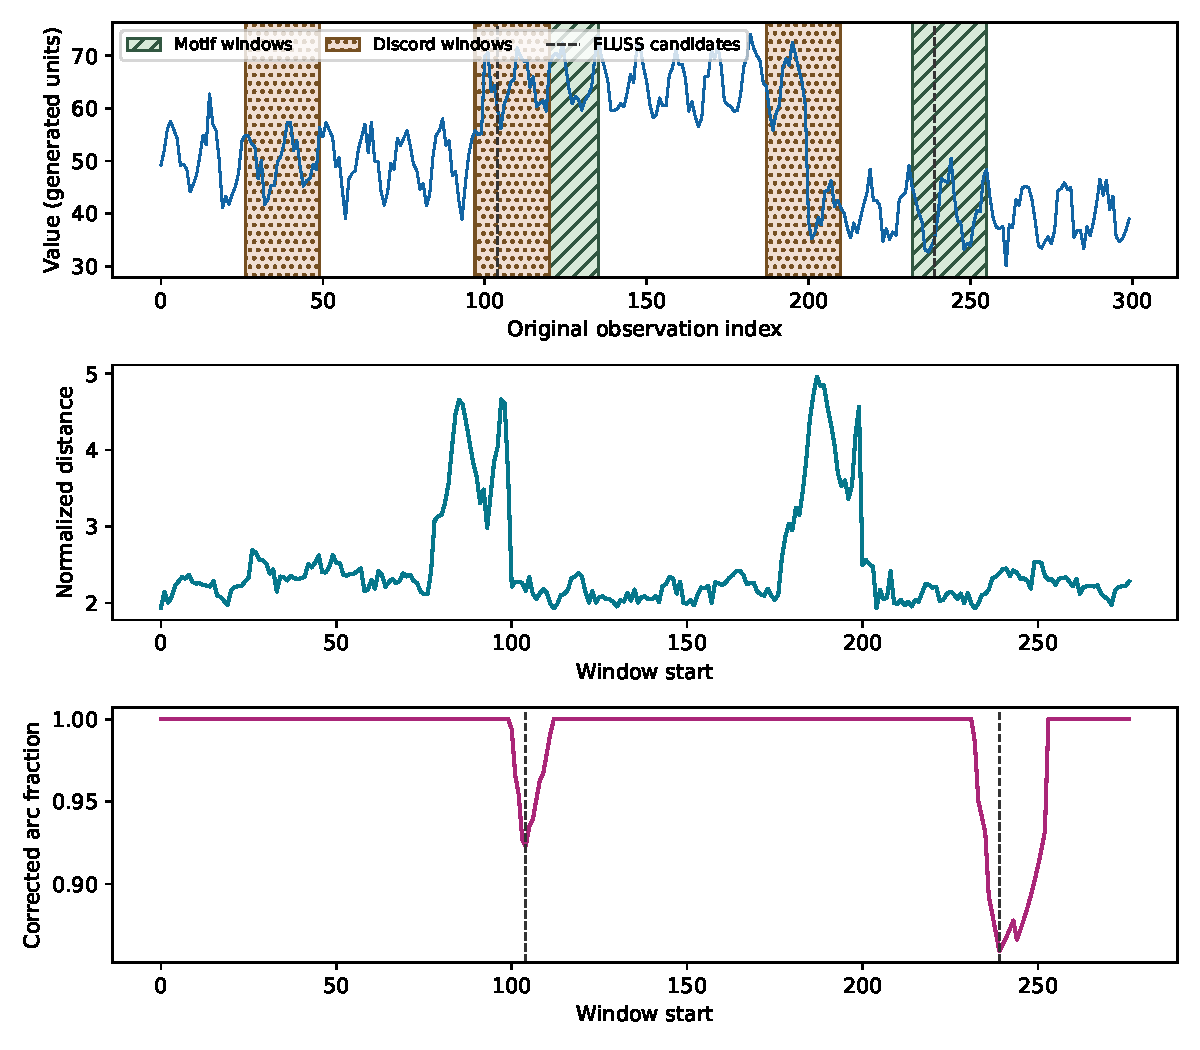
\includegraphics[width=.95\linewidth]{sequence-patterns.pdf}
\caption{Original-axis sequence annotations for the structural-break case. Hatched spans label the motif and discord windows, and dashed boundaries mark FLUSS candidates. Neither the window ranks nor the requested segmentation count establishes ground-truth anomalies.}\label{fig:sequence-patterns}\end{figure}

Costa multiscale entropy averages non-overlapping blocks at each scale $\tau$~\cite{costa}. Sample entropy uses order two, tolerance $r=0.15s(x)$ fixed to the original population standard deviation, and the same $N_\tau-2$ template starts for dimensions two and three. Distinct unordered pairs match at Chebyshev distance at most $r$, excluding self matches. If $B_\tau$ pairs match at dimension two and $A_\tau$ extensions match, the estimate is
\begin{equation}
 \operatorname{SampEn}_\tau=-\log(A_\tau/B_\tau).
\end{equation}
Fewer than twenty coarse observations, or no matching extensions, yield an unavailable estimate with a reason and exported counts. An unavailable value is not zero complexity. Constant sequences give zero where all eligible templates match.

Binary Lempel--Ziv complexity uses $1[x_t>\operatorname{median}(x)]$, assigning ties to zero. Both phrase count $c(n)$ and $c(n)\log_2(n)/n$ are retained~\cite{lz}. The asymptotic normalization is not clipped to one. Time-reversal asymmetry reports the mean of $x_{t+\ell}(x_{t+2\ell}^2-x_t^2)$ at lags one, two and seven, where available, on raw and standardized observations. Raw units are cubed source units. Reversal changes the sign, but a finite nonzero statistic alone is not a significance test or an irreversibility test.

Figure~\ref{fig:sequence-entropy} shows the entropy calculation as coarsening reduces available template counts; its curve is not a calibrated measure of forecasting ability.

\begin{figure}[ht]\centering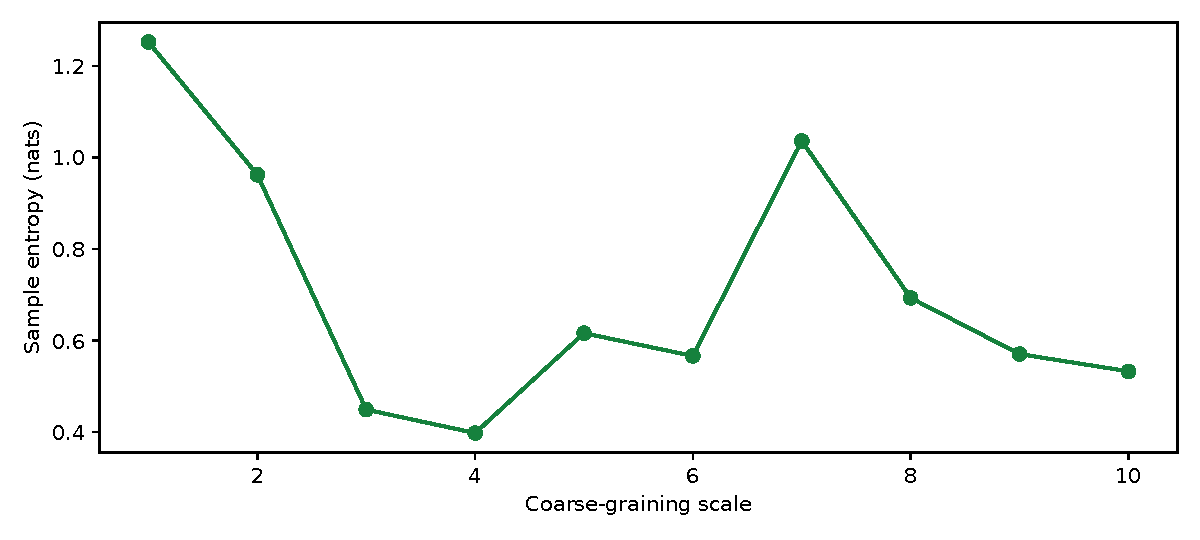
\includegraphics[width=.8\linewidth]{sequence-entropy.pdf}
\caption{Multiscale entropy on the structural-break case with the original tolerance fixed across scales. Coarse sequence lengths decrease with scale; finite-sample availability and matching counts remain part of the interpretation.}\label{fig:sequence-entropy}\end{figure}

The previous nolds correlation-dimension and Lyapunov defaults used randomized RANSAC fits without an explicit random state. The adapter now obtains deterministic log-distance fitting data, then fits the same robust polynomial-feature linear model with an explicit local seed. Least squares is the fallback when consensus fails. A case seed is derived from SHA-256 of case identity and the supplied pipeline seed; surrogate and 0--1 calculations receive derived local seeds. Process-global random state is not changed. DFA and fallback R/S slopes explicitly request least squares. These fit choices can move historical diagnostics even when the source observations are unchanged. Two complete analyzer calls for every case must serialize identically before promotion; independent-process and caller-RNG tests additionally protect the estimator boundary. The existing surrogate gate remains necessary for a chaos classification.

\subsection{Corpus forecastability and disjoint-series confirmation}
\label{sec:forecastability}
A separate fixed-protocol experiment processes the complete Monash M4 Daily source, 4,227 series under CC BY 4.0~\cite{m4daily}. Every identity is admitted or assigned an explicit exclusion. Exact whole-sequence duplicates retain the lexicographically first identity for inference. Nonfinite observations, insufficient prefixes and unavailable MASE denominators are excluded with reasons. Source ZIP and extracted TSF hashes identify the input bytes; a full-sequence identity hash is used only for duplicate grouping and partition allocation, never as a predictor.

Each admitted series contributes three non-overlapping fourteen-step future blocks. Each model uses at most the preceding 1,024 contiguous observations at an origin. Features use only the earliest fitting prefix. Forecast seasonality is one, matching the M4 Daily setting; weekly phase strength is a separately named diagnostic. The fixed roster is Naive, SeasonalNaive, SES, Holt, HoltWinters, Theta, AutoETS and AutoTheta. Some configurations coincide when the period is one; these explicit identities do not imply eight distinct future paths. No deep or pretrained model participates in this corpus study, which does not replace the separate twenty-two-variant case experiment.

Model MASE is averaged over the three origins within each series. The association target is $\log(1+\min_k\overline{\operatorname{MASE}}_k)$ over the fixed roster. This is an optimistic within-roster oracle, not inherent predictability. Forty prefix diagnostics include catch24, location/scale and ordering summaries, multiscale entropy, binary complexity, reversal asymmetry and profile distances. Associations may reflect a scaled-error denominator or source grouping rather than a causal forecasting mechanism.

Exact sequence identities allocate approximately seventy percent of series to discovery and the rest to confirmation. Kendall tests use available feature values and aggregate series targets. Benjamini--Yekutieli correction treats the entire feature family separately in each partition at $q=0.05$~\cite{freshby}. In sorted order, adjusted probabilities use
\begin{equation}
 q_{(i)}=\min_{j\ge i}\left\{1,\frac{K H_K}{j}p_{(j)}\right\},\qquad H_K=\sum_{k=1}^{K}k^{-1}.
\end{equation}
Confirmation requires rejection in both partitions and matching effect direction. All feature counts, signed effects, raw probabilities, adjusted probabilities and negative decisions are retained. Series are the statistical units; origins are not treated as independent replications. Related industries or latent sources can still violate observation-independence assumptions after exact deduplication.

A fixed random forest predicts the best model identity from discovery features, with 200 trees, maximum depth eight, minimum leaf size ten and random state 42. Missing-value medians and the constant comparator are fitted on discovery only. Confirmation outcomes choose neither parameters nor feature thresholds. The selected rule is compared once on confirmation series with that constant method and the future-informed per-series oracle. Scores are descriptive held-out results, not population-superiority or operational guarantees. Negative selection outcomes remain in the report.

The complete source contains 4,227 identities; 4,226 are admitted and 1 is explicitly excluded. The deterministic partitions contain 2,946 discovery and 1,280 confirmation series. Of forty tested features, 21 meet the fixed two-partition confirmation rule. The discovery-selected constant is AutoETS. On confirmation series, the fixed selector has mean MASE 3.3501, the constant 3.2570, and the future-informed oracle 3.0005. The selector's error is 0.0931 higher than the constant on this fixed split. This descriptive outcome is not a significance test of selection benefit. The oracle uses future outcomes and cannot be deployed as a selection policy.

Exclusions by reason: zero or unavailable MASE scale: 1.

\begin{center}\begin{tabular}{lr}
\toprule Confirmation method & Mean MASE\\\midrule
AutoTheta & 3.2195 \\
Naive & 3.2216 \\
SeasonalNaive & 3.2216 \\
Theta & 3.2228 \\
SES & 3.2263 \\
AutoETS & 3.2570 \\
Holt & 3.6217 \\
HoltWinters & 3.6217 \\
\bottomrule\end{tabular}\end{center}

\clearpage
Table~\ref{tab:corpus-associations} retains all forty tested prefix features and the adjusted probabilities in both partitions, rather than showing only the twenty-one confirmations.
\begingroup\footnotesize\setlength{\tabcolsep}{3pt}
\begin{longtable}{p{.35\textwidth}rrrrrr}
\caption{All forty prespecified features. D/C denote discovery/confirmation. Signed Kendall effects, BY-adjusted probabilities and the fixed confirmation decision are retained, including negative outcomes. Available counts and raw probabilities are in the public artifact.}\label{tab:corpus-associations}\\
\toprule Feature & $n_D$ & $\tau_D$ & $q_D$ & $n_C$ & $\tau_C$ & $q_C$\\\midrule\endfirsthead
\toprule Feature & $n_D$ & $\tau_D$ & $q_D$ & $n_C$ & $\tau_C$ & $q_C$\\\midrule\endhead
\raggedright \nolinkurl{acf_1} & 2946 & 0.012 & 1 & 1280 & 0.032 & 0.5 \\
\raggedright \nolinkurl{acf_7} & 2946 & -0.004 & 1 & 1280 & 0.017 & 1 \\
\raggedright \nolinkurl{catch24_CO_Embed2_Dist_tau_d_expfit_meandiff}\textsuperscript{*} & 2946 & 0.126 & 4.8e-23 & 1280 & 0.154 & 7.4e-15 \\
\raggedright \nolinkurl{catch24_CO_FirstMin_ac} & 2946 & -0.063 & 3.4e-06 & 1280 & -0.049 & 0.068 \\
\raggedright \nolinkurl{catch24_CO_HistogramAMI_even_2_5} & 2946 & 0.006 & 1 & 1280 & 0.004 & 1 \\
\raggedright \nolinkurl{catch24_CO_f1ecac}\textsuperscript{*} & 2946 & -0.094 & 4e-13 & 1280 & -0.079 & 0.00023 \\
\raggedright \nolinkurl{catch24_CO_trev_1_num}\textsuperscript{*} & 2946 & 0.145 & 4.7e-30 & 1280 & 0.173 & 3.9e-18 \\
\raggedright \nolinkurl{catch24_DN_HistogramMode_10} & 2946 & -0.021 & 0.5 & 1280 & -0.047 & 0.086 \\
\raggedright \nolinkurl{catch24_DN_HistogramMode_5} & 2946 & -0.029 & 0.12 & 1280 & -0.044 & 0.12 \\
\raggedright \nolinkurl{catch24_DN_Mean} & 2946 & -0.035 & 0.03 & 1280 & -0.045 & 0.1 \\
\raggedright \nolinkurl{catch24_DN_OutlierInclude_n_001_mdrmd}\textsuperscript{*} & 2946 & -0.042 & 0.0044 & 1280 & -0.059 & 0.014 \\
\raggedright \nolinkurl{catch24_DN_OutlierInclude_p_001_mdrmd}\textsuperscript{*} & 2946 & 0.136 & 1.6e-26 & 1280 & 0.167 & 2.6e-17 \\
\raggedright \nolinkurl{catch24_DN_Spread_Std} & 2946 & -0.034 & 0.034 & 1280 & -0.044 & 0.12 \\
\raggedright \nolinkurl{catch24_FC_LocalSimple_mean1_tauresrat}\textsuperscript{*} & 2946 & 0.117 & 3.7e-20 & 1280 & 0.120 & 3.5e-09 \\
\raggedright \nolinkurl{catch24_FC_LocalSimple_mean3_stderr} & 2946 & -0.003 & 1 & 1280 & -0.023 & 1 \\
\raggedright \nolinkurl{catch24_IN_AutoMutualInfoStats_40_gaussian_fmmi}\textsuperscript{*} & 2946 & -0.088 & 1.2e-08 & 1280 & -0.106 & 1.7e-05 \\
\raggedright \nolinkurl{catch24_MD_hrv_classic_pnn40} & 2946 & 0.010 & 1 & 1280 & -0.005 & 1 \\
\raggedright \nolinkurl{catch24_PD_PeriodicityWang_th0_01}\textsuperscript{*} & 2946 & -0.077 & 3.2e-08 & 1280 & -0.098 & 9.9e-06 \\
\raggedright \nolinkurl{catch24_SB_BinaryStats_diff_longstretch0}\textsuperscript{*} & 2946 & -0.074 & 2.2e-07 & 1280 & -0.099 & 1e-05 \\
\raggedright \nolinkurl{catch24_SB_BinaryStats_mean_longstretch1}\textsuperscript{*} & 2946 & -0.110 & 1e-17 & 1280 & -0.098 & 3.8e-06 \\
\raggedright \nolinkurl{catch24_SB_MotifThree_quantile_hh} & 2946 & 0.006 & 1 & 1280 & -0.000 & 1 \\
\raggedright \nolinkurl{catch24_SB_TransitionMatrix_3ac_sumdiagcov}\textsuperscript{*} & 2946 & 0.046 & 0.0031 & 1280 & 0.085 & 0.00017 \\
\raggedright \nolinkurl{catch24_SC_FluctAnal_2_dfa_50_1_2_logi_prop_r1}\textsuperscript{*} & 2946 & -0.080 & 3.6e-09 & 1280 & -0.098 & 8.1e-06 \\
\raggedright \nolinkurl{catch24_SC_FluctAnal_2_rsrangefit_50_1_logi_prop_r1} & 2946 & 0.001 & 1 & 1280 & -0.035 & 0.44 \\
\raggedright \nolinkurl{catch24_SP_Summaries_welch_rect_area_5_1}\textsuperscript{*} & 2946 & -0.064 & 2.2e-06 & 1280 & -0.054 & 0.029 \\
\raggedright \nolinkurl{catch24_SP_Summaries_welch_rect_centroid}\textsuperscript{*} & 2946 & 0.097 & 1.8e-11 & 1280 & 0.076 & 0.0025 \\
\raggedright \nolinkurl{history_length}\textsuperscript{*} & 2946 & -0.149 & 7.8e-26 & 1280 & -0.156 & 1.4e-12 \\
\raggedright \nolinkurl{kurtosis} & 2946 & 0.029 & 0.11 & 1280 & 0.046 & 0.093 \\
\raggedright \nolinkurl{linear_trend_r}\textsuperscript{*} & 2946 & 0.114 & 3.8e-19 & 1280 & 0.147 & 1.4e-13 \\
\raggedright \nolinkurl{log_std} & 2946 & -0.035 & 0.034 & 1280 & -0.044 & 0.12 \\
\raggedright \nolinkurl{lz_binary}\textsuperscript{*} & 2946 & 0.041 & 0.007 & 1280 & 0.057 & 0.02 \\
\raggedright \nolinkurl{mse_1} & 2946 & 0.002 & 1 & 1280 & -0.006 & 1 \\
\raggedright \nolinkurl{mse_10} & 2476 & 0.020 & 0.76 & 1071 & -0.017 & 1 \\
\raggedright \nolinkurl{mse_2} & 2941 & 0.009 & 1 & 1278 & 0.003 & 1 \\
\raggedright \nolinkurl{mse_5} & 2834 & 0.010 & 1 & 1223 & 0.020 & 1 \\
\raggedright \nolinkurl{profile_max} & 2946 & 0.018 & 0.87 & 1280 & 0.014 & 1 \\
\raggedright \nolinkurl{profile_median}\textsuperscript{*} & 2946 & -0.050 & 0.00041 & 1280 & -0.056 & 0.022 \\
\raggedright \nolinkurl{reversal_1}\textsuperscript{*} & 2946 & 0.130 & 2e-24 & 1280 & 0.141 & 1.3e-12 \\
\raggedright \nolinkurl{skewness}\textsuperscript{*} & 2946 & 0.083 & 1.6e-10 & 1280 & 0.094 & 8.1e-06 \\
\raggedright \nolinkurl{weekly_phase_strength}\textsuperscript{*} & 2946 & 0.090 & 3.3e-12 & 1280 & 0.086 & 5.5e-05 \\
\bottomrule\end{longtable}
* Rejected at BY $q\leq0.05$ in both partitions with the same effect direction.\endgroup


\begin{samepage}
The evaluator retains external per-origin forecast-path audits and independently rescores every exported MASE before compact export. Its resumable cache binds source bytes, fixed protocol, implementation and package identities. Admission independently checks inventory, duplicate separation, temporal schedules, discovery-only imputation, aggregate scores, corrected probabilities and Kendall effects. The public notebook retrains the selector from admitted discovery rows and repeats reference statistical calculations without claiming a new fit of the eight external-corpus forecasting models. These layers distinguish full forecasting reproduction, compact-table statistical reproduction and browser inspection.\par
\end{samepage}


Figure~\ref{fig:corpus-selection} puts the discovery-trained selector beside the fixed comparison and the future-informed oracle, retaining the unfavorable held-out selection result.

\begin{figure}[ht]\centering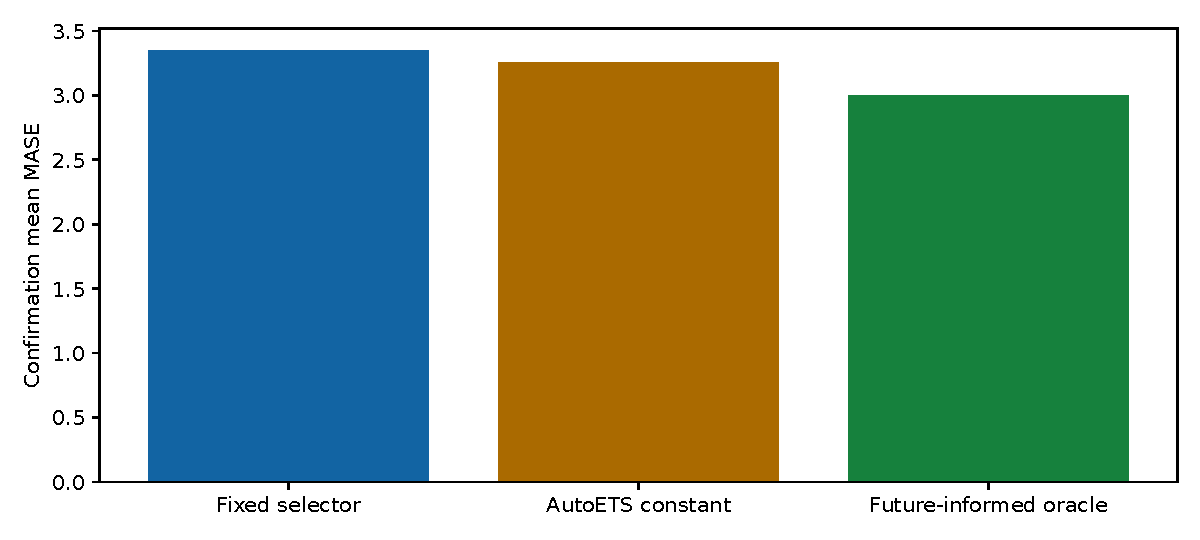
\includegraphics[width=.85\linewidth]{corpus-selection.pdf}
\caption{Mean MASE on confirmation series for the fixed discovery-trained selector, the discovery-selected constant method and the future-informed oracle. Bars are descriptive averages over the same admitted confirmation rows; they are not confidence intervals.}\label{fig:corpus-selection}\end{figure}


\section{Held-out calibration of the browser linear forecast}
\label{sec:browser-calibration}

The browser forecast is a global linear map fitted to synthetic windows, not
the locally trained neural implementation that shares the NLinear name in the
offline comparison. This distinction matters because a name does not identify
a loss function, a training sample or an uncertainty procedure. The original
browser matrix has 48 input coordinates and 12 output coordinates. It is
estimated by least squares on 52,144 overlapping windows drawn from 400
generated series. Its point forecasts run through an actual ONNX matrix
multiplication in the browser. Neither this small representation nor its
execution speed establishes that its forecast distribution is calibrated.

In the previous implementation, a pooled training-residual standard deviation
was multiplied by the observed window's scale and by the square root of the
forecast lead. This rule produces finite bands, but no held-out experiment had
established their nominal coverage. Training residuals reuse outcomes that
helped estimate the map; pooling leads also discards the error distribution's
dependence on forecast distance. Multiplying that pooled scale by another
lead-dependent factor is an engineering approximation rather than a consequence
of the fitted global regression. The following experiments evaluate that
specific implemented rule. They do not treat Gaussian intervals as a uniformly
weak baseline or extrapolate their behavior to every model with Gaussian errors.

The first experiment tested a fixed regularization grid and independent
calibration. Its point-error result was unfavorable. A second, separately
specified experiment therefore retained the original point matrix and tested
prefix-stratified interval calibration on fresh generated series. This sequence
separates an observed failure from a new confirmation. It does not permit the
first test set to become the second experiment's tuning set while still being
described as independent confirmation. The complete first result remains in
the record, including its validation decision and family-specific coverage.

\subsection{Observed-window normalization and a fixed point map}
\label{sec:browser-normalization}

Let $x=(x_1,\ldots,x_L)$ be the last $L=48$ observations and let $a_h$ denote
the target at lead $h\in\{1,\ldots,12\}$. All normalization quantities are
computed from $x$, before any target is revealed. Define
\begin{equation}
 \bar x=L^{-1}\sum_{i=1}^L x_i,\qquad
 s(x)=\left[L^{-1}\sum_{i=1}^L(x_i-\bar x)^2\right]^{1/2},\qquad
 z_i=\frac{x_i-x_L}{s(x)}.
 \label{eq:browser-normalization}
\end{equation}
For a matrix $W\in\mathbb R^{L\times H}$, the normalized prediction is
$\hat u=z^\top W$ and the prediction in the observation's units is
\begin{equation}
 \hat a_h=x_L+s(x)\hat u_h.
 \label{eq:browser-inverse}
\end{equation}
The matrix contains no intercept. Subtraction of the last observation fixes the
origin used by the exported model; subtraction of the sample mean would define
a different predictor. The denominator is the population standard deviation of
the observed window, not the residual standard deviation of a trend fit. The
training recipe and browser implementation use this same convention.

If $s(x)=0$, the normalized model is unavailable. Substituting a raw-unit scale
of one would change the computation when the same constant sequence is expressed
in different units. A constant sequence can be forecast by a separately declared
constant predictor, but that is not evidence for assigning a calibrated
uncertainty scale to this normalized map. Nonfinite observations, unsupported
horizons and malformed matrix outputs are also refused. The 12-lead model does
not generate additional leads by repeating its last output.

The deployed matrix is preserved byte-for-byte throughout both experiments.
Its SHA-256 is recorded with the calibration metadata, and the browser verifies
the actual downloaded graph against that digest before inference. This prevents
a valid calibration array from being accidentally paired with a different
point map. Numerical parity is checked independently using the float32 graph
and a NumPy multiplication. Agreement of those computations is a numerical
identity check; it is not a forecasting-performance claim.

\subsection{Regularization, selection and the first held-out experiment}
\label{sec:browser-ridge}

The training collection uses the original generator and random sequence. Each
series is assigned one of four equally probable mechanisms: sinusoidal
seasonality, trend plus seasonality, trend, or independent noise. Periods are
selected from six, twelve and twenty-four observations; series lengths are
sampled from the integer interval $[120,260)$. These are controlled mechanisms,
not observations from the electricity, air-quality or competition datasets.
The overlapping windows within one training series share observations. They
therefore cannot be used as independent calibration or test replications.

For normalized training rows $Z$ and targets $U$, the candidate family minimizes
\begin{equation}
 \widehat W_\lambda=\mathop{\rm argmin}_{W}
 \left\{\frac{1}{N}\|U-ZW\|_F^2+\lambda\|W\|_F^2\right\}.
 \label{eq:browser-ridge}
\end{equation}
The fixed grid is $\{0,10^{-6},10^{-4},10^{-2},10^{-1},1,10\}$. The zero entry
uses a least-squares solver, including when the Gram matrix is singular.
Positive penalties solve the regularized normal equations. Candidate matrices
are converted to float32 before validation. Selection minimizes mean normalized
squared error on the final complete window of each of 200 independent
validation series. Exact ties select the earlier grid entry. The selected
matrix is not refitted using the validation or calibration series.

Four hundred additional series supply calibration errors and another four
hundred supply test errors. A series contributes only its final complete
48-to-12 window outside training. The training, validation, calibration and test
generators use local PCG64 seeds 20260704, 20261105, 20261106 and 20261107,
respectively. These integers identify generator streams; they are not dates of
data collection. Full-sequence hashes verify that no series is duplicated
across any partition. Family labels are retained for evaluation, but do not
enter the fitted linear map.

Validation selected $\lambda=0.1$. On the independent test sample, normalized
mean squared error was 0.550561, compared with 0.548742 for the frozen original
map. The paired difference was $+0.001819$, with an exploratory 95\% series
bootstrap interval $[0.000145,0.003465]$. Only 150 of 400 series had lower
squared loss. Thus the validation-selected ridge candidate did not improve the
point forecast in this experiment. This outcome is retained rather than
replaced by the favorable validation score or a new penalty chosen from test
outcomes. A repeat-last control had normalized squared error 1.795089, which
locates both linear maps relative to a simpler forecast without making either
map an unconditional winner outside this generator.

\subsection{Per-lead split calibration and its conditional limits}
\label{sec:browser-split}

For a fixed point model and independent calibration series indexed by $j$,
define the absolute normalized error at lead $h$ as
\begin{equation}
 R_{jh}=\left|\frac{a_{jh}-\hat a_{jh}}{s(x_j)}\right|.
 \label{eq:browser-residual}
\end{equation}
With $n$ calibration series and miscoverage $\alpha=0.2$, the radius is the
$k$th order statistic,
\begin{equation}
 k=\lceil(n+1)(1-\alpha)\rceil,\qquad
 q_h=R_{(k)h},\qquad
 I_h(x)=[\hat a_h-s(x)q_h,\hat a_h+s(x)q_h].
 \label{eq:browser-radius}
\end{equation}
If $k>n$, a finite empirical radius is not available under this convention.
Interpolation of the nominal 80th percentile is not substituted for the
specified finite-sample rank. For $n=400$, the selected one-based rank is 321.
Calibration uses the actual runtime output of the exported point model, so
calibration and testing apply the same numerical predictor.

For independent exchangeable calibration and test series and a point model
fixed before calibration, the rank of the new residual among the $n+1$
residuals is uniform in the absence of ties; conservative tie handling gives
the usual lower coverage bound. Consequently
\begin{equation}
 \Pr\{a_h\in I_h(x)\}\geq 1-\alpha.
 \label{eq:browser-marginal-guarantee}
\end{equation}
This is a marginal statement over new series from the same population,
separately for each lead~\cite{splitintro}. It does not say that all twelve
future observations are covered together with probability 0.8. Nor does it
guarantee 0.8 conditional coverage for each observed prefix, each latent
generator family or an arbitrary authentic series. Internal serial dependence
within one generated series does not by itself invalidate exchangeability
across independently generated series; pooling dependent windows as separate
calibration observations would be a different design.

In the first test sample, the calibrated ridge intervals had 79.46\% overall
coverage, normalized mean width 1.659786 and normalized interval score 2.781262.
The original Gaussian rule had 96.60\% coverage, width 4.593046 and score
4.764406. However, the calibrated candidate's white-noise coverage was only
53.06\%, while seasonal and trend-plus-seasonal coverage exceeded 93\%.
The aggregate result therefore could not support a statement that all
mechanisms were calibrated. It motivated a new prefix-stratified procedure
and a fresh confirmation population, while leaving the original result intact.

\subsection{Prefix-roughness strata and independent confirmation}
\label{sec:browser-strata}

The second experiment changes intervals while preserving exactly the original
point predictions. Its observable grouping statistic is
\begin{equation}
 \rho(x)=\frac{(L-1)^{-1}\sum_{i=1}^{L-1}(x_{i+1}-x_i)^2}
 {L^{-1}\sum_{i=1}^L(x_i-\bar x)^2}.
 \label{eq:browser-roughness}
\end{equation}
The three fixed bins are $[0,0.5)$, $[0.5,1.25)$ and $[1.25,\infty)$.
This ratio compares local changes with total observed variation. Independent
noise has population ratio near two; a well-sampled sinusoid has ratio
approximately $2\{1-\cos(2\pi/m)\}$. These relationships motivate separating
smooth, oscillatory and rough prefixes without using a hidden mechanism label.
The boundaries are engineering choices fixed before the new confirmation
outcomes, rather than estimated cut points optimized on those outcomes.

For a bin $b$, the calibration radius uses only series whose observed prefixes
belong to $b$:
\begin{equation}
 q_{bh}=R_{(k_b)h}^{(b)},\qquad
 k_b=\lceil(n_b+1)(1-\alpha)\rceil.
 \label{eq:browser-group-radius}
\end{equation}
At least twenty independent calibration series are required in every bin.
Conditional on a fixed prefix partition and exchangeable series within a bin,
the rank argument applies separately in that bin. It does not acquire validity
within every latent family simply because the bin was computed from a prefix.
The number of calibration series per bin affects the granularity and sampling
variability of each radius; finer partitions can therefore reduce efficiency
or leave a bin without an admissible radius.

The confirmation uses 400 new calibration series from seed 20261109 and 800
new test series from seed 20261110. Their full-sequence hashes are disjoint
from all 1,400 series in the first experiment. The point map is not trained,
selected or updated in this confirmation. Its Gaussian, globally calibrated
and prefix-stratified interval arms use identical points at every test origin.
Calibration bin counts were 115, 120 and 165. This yields finite-sample ranks
93, 97 and 133, respectively. The global arm uses all 400 calibration series
and provides a matching ablation of the prefix partition.

\begin{algorithm}[htbp]
\caption{Fixed-point forecast with prefix-stratified marginal intervals. Every
quantity used at prediction time is determined before observing the next target.}
\label{alg:browser-calibration}
\begin{algorithmic}[1]
\Require Frozen point matrix $W$, independently calibrated radii $q_{bh}$,
observed prefix $x$, supported horizon $H=12$
\State Refuse nonfinite observations, an incomplete lookback or $s(x)\leq0$
\State Compute $z$ from Equation~\ref{eq:browser-normalization}
\State Select the fixed bin $b$ containing $\rho(x)$
\State Compute $\hat u=z^\top W$ using the verified float32 ONNX graph
\For{$h=1,\ldots,H$}
\State Set $\hat a_h=x_L+s(x)\hat u_h$
\State Store $I_h=[\hat a_h-s(x)q_{bh},\hat a_h+s(x)q_{bh}]$
\EndFor
\State \textbf{return} $(I_1,\ldots,I_H)$
\end{algorithmic}
\end{algorithm}

Algorithm~\ref{alg:browser-calibration} requires $O(LH+L)$ arithmetic after
the small fixed graph has been loaded. It carries no recurrent hidden state
and performs no online refit. Hash verification binds the graph to the radii;
it does not identify whether a new series belongs to the calibration
population. The browser therefore describes the intervals as nominal marginal
bands calibrated on synthetic prefixes, with authentic-data coverage
unconfirmed. Changing the requested horizon or nominal level requires new
calibration metadata instead of silently extrapolating the existing arrays.

\subsection{Scores, uncertainty and confirmation outcomes}
\label{sec:browser-results}

Each test series receives equal weight. Point errors are divided by the
observed lookback standard deviation and then squared or taken in absolute
value. These are normalized errors, not MASE. For lower and upper bounds
$\ell_{jh}$ and $u_{jh}$, the normalized interval score is
\begin{equation}
 \operatorname{NIS}_j=\frac{1}{Hs(x_j)}\sum_{h=1}^H
 \left[(u_{jh}-\ell_{jh})+
 \frac{2}{\alpha}(\ell_{jh}-a_{jh})_+
 +\frac{2}{\alpha}(a_{jh}-u_{jh})_+\right].
 \label{eq:browser-score}
\end{equation}
It penalizes both width and misses, rather than rewarding coverage without
regard to efficiency. The normalization is not the seasonal-naive denominator
used by MSIS elsewhere in this report. Comparisons are made within this
experiment and are not pooled with differently scaled losses from the external
forecast-combination study.

\begin{table}[htbp]\centering
\caption{Independent synthetic confirmation on 800 new series. All three
interval arms use identical frozen point forecasts and the same observed-prefix
normalization; smaller interval scores represent more efficient predictions.}
\label{tab:browser-confirmation}
\begin{tabular}{lrrr}\toprule
Quantity & Gaussian & Global & Stratified\\\midrule
Normalized squared error & 0.548553 & 0.548553 & 0.548553\\
Marginal coverage & 0.970521 & 0.834583 & 0.827292\\
Normalized width & 4.593046 & 1.873393 & 1.738557\\
Normalized interval score & 4.749003 & 2.803800 & 2.393376\\\bottomrule
\end{tabular}\end{table}

Table~\ref{tab:browser-confirmation} shows a 49.60\% reduction in mean interval
score relative to the current Gaussian rule and a 14.64\% reduction relative
to global calibration. These improvements concern intervals around unchanged
point forecasts. Figure~\ref{fig:browser-efficiency} separates interval score
from width: a narrower band is not automatically better if its miss penalties
increase. In this confirmation, stratification reduces both the mean width and
the mean proper interval score relative to global calibration.

\begin{figure}[htbp]\centering
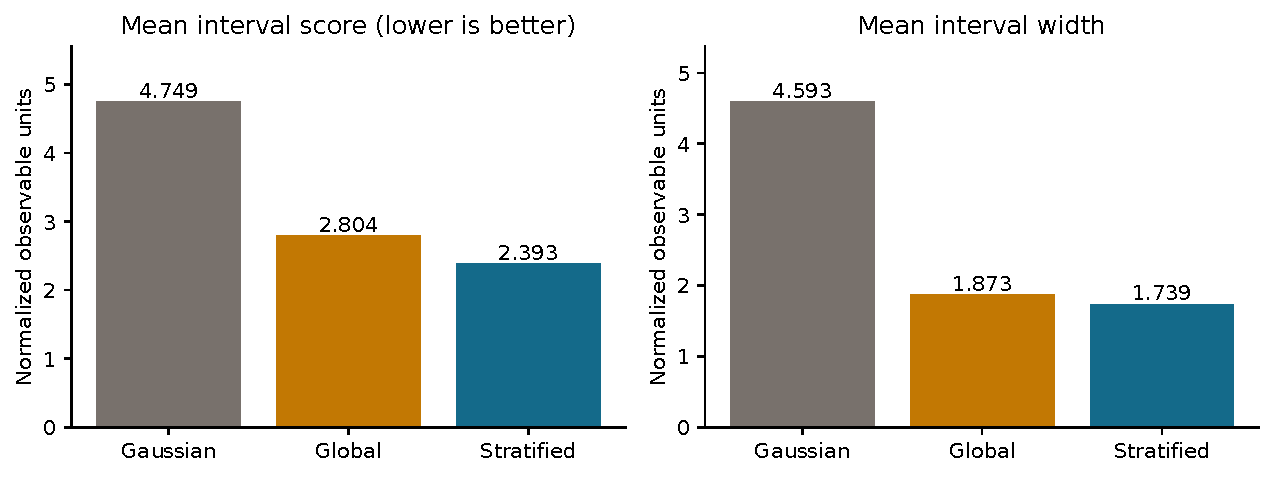
\includegraphics[width=\textwidth]{browser-interval-efficiency.pdf}
\caption{Mean interval score and width from all 800 independent confirmation
series. The three procedures share point forecasts; these plotted means do not
represent independently estimated confidence intervals.}
\label{fig:browser-efficiency}\end{figure}

Uncertainty is summarized by drawing 10,000 paired bootstrap samples of the
800 complete series with local PCG64 seed 20261108. Within a draw, the same
series indices are used for both interval procedures. Forecast leads are not
resampled as independent observations. The stratified-minus-Gaussian mean
interval-score difference is $-2.355627$, with exploratory 95\% percentile
interval $[-2.437258,-2.273077]$. The stratified-minus-global difference is
$-0.410424$, with interval $[-0.451789,-0.368795]$. These are unadjusted
exploratory intervals under the experiment's independent-series design, not
multiplicity-controlled evidence about every reported subgroup. Respectively,
778 and 606 of 800 series have strictly lower interval score, so the mean
advantage does not conceal a majority of series with larger losses.

\begin{figure}[htbp]\centering
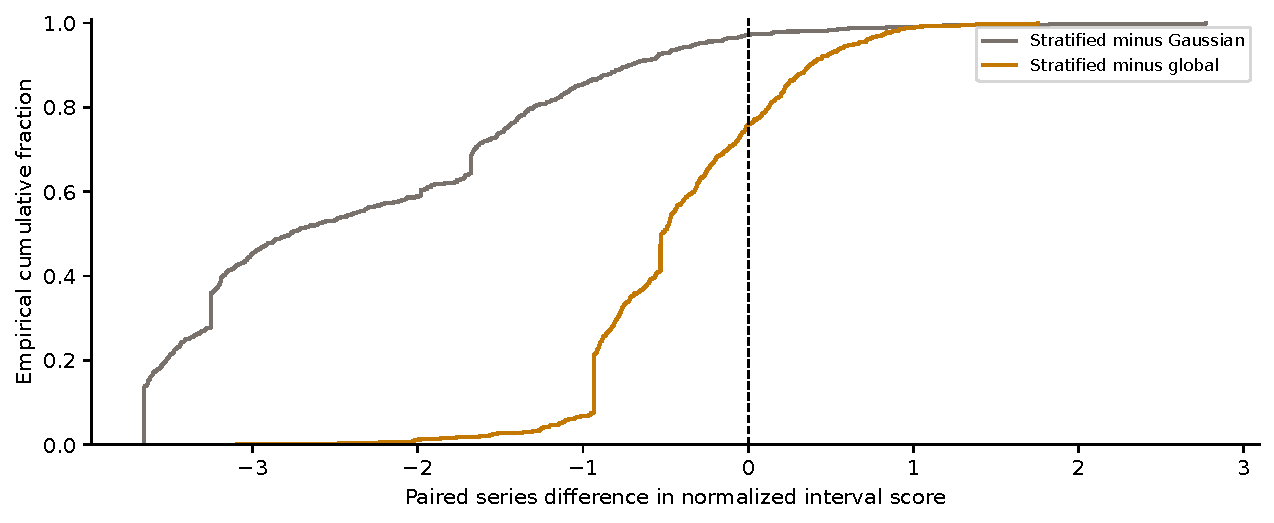
\includegraphics[width=\textwidth]{browser-paired-scores.pdf}
\caption{Empirical distributions of paired interval-score differences for
individual confirmation series. Negative values favor prefix stratification;
the positive tails retain series on which the comparison is unfavorable.}
\label{fig:browser-paired}\end{figure}

Figure~\ref{fig:browser-paired} makes the individual-loss distribution visible
alongside its aggregate uncertainty. Some prefixes benefit little and some
have larger interval penalties after stratification. No series is removed
because its interval score worsens. The empirical distribution is a description
of these 800 generated series; its tails cannot establish the frequency of
rare failures in an operational population absent from the generator.

\begin{table}[htbp]\centering
\caption{Prefix-bin calibration support and held-out coverage. Fixed bins use
observed histories alone; their coverage summaries do not guarantee validity
for every hidden generating mechanism or individual prefix.}
\label{tab:browser-groups}
\begin{tabular}{lrr}\toprule
Observed-prefix roughness & Calibration series & Test coverage\\\midrule
$[0,0.5)$ & 115 & 0.843377\\
$[0.5,1.25)$ & 120 & 0.804773\\
$[1.25,\infty)$ & 165 & 0.826786\\\bottomrule
\end{tabular}\end{table}

Table~\ref{tab:browser-groups} reports coverage in the observable bins targeted
by the stratified construction. Family-specific results remain distinct.
Coverage is 80.46\% for noise, 74.57\% for trend, 86.71\% for seasonality and
88.92\% for trend plus seasonality. Figure~\ref{fig:browser-families} shows
that stratification addresses the large noise-family shortfall of global
calibration without eliminating all family differences. In particular, the
trend family remains below nominal coverage. These family outcomes were not
used to redraw the bins after the confirmation was scored.

\begin{figure}[htbp]\centering
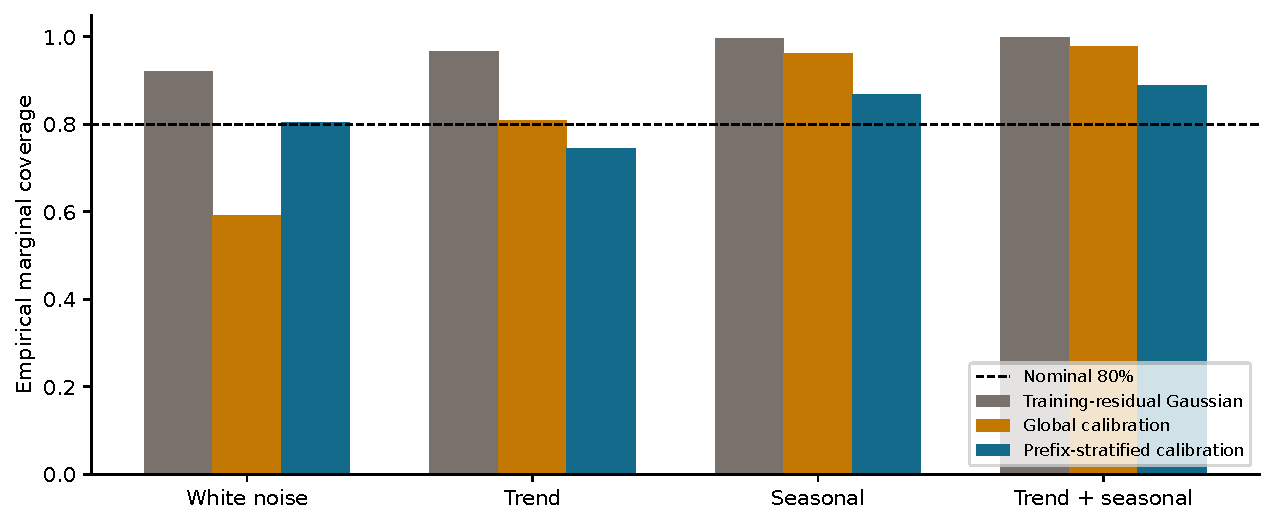
\includegraphics[width=\textwidth]{browser-family-coverage.pdf}
\caption{Confirmation coverage by latent generator family for identical point
forecasts. Prefix stratification improves the noise-family shortfall, while
the trend family's remaining undercoverage prevents a universal calibration claim.}
\label{fig:browser-families}\end{figure}

Figure~\ref{fig:browser-leads} shows lead-specific coverage, ranging from
79.50\% to 85.13\% for the stratified rule. Separate marginal radii allow
different error distributions at different leads. They do not force a
monotone square-root growth law and do not imply a joint prediction region.
The experiment's prospectively fixed engineering criteria require identical
point forecasts, adequate calibration support, lower mean interval score,
overall coverage between 75\% and 85\%, bin coverage between 70\% and 90\%,
and normalized runtime error below $10^{-4}$. All six passed. This admission
decision is explicitly weaker than demonstrating calibration on real data.

\begin{figure}[htbp]\centering
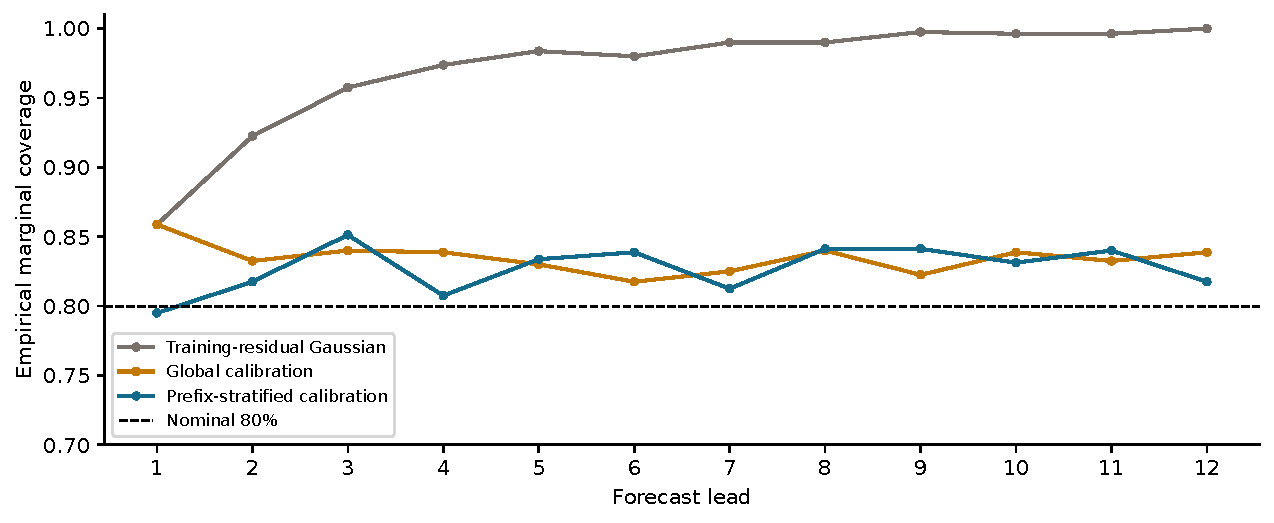
\includegraphics[width=\textwidth]{browser-lead-coverage.pdf}
\caption{Empirical coverage at each of twelve future leads. The dashed line
marks nominal marginal coverage; the graph does not report simultaneous
coverage of an entire forecast trajectory.}
\label{fig:browser-leads}\end{figure}

\subsection{Unit invariance, reproducibility and applicability}
\label{sec:browser-validation}

Consider a positive change of units and location, $x'_i=ax_i+b$, $a>0$.
Then $s(x')=as(x)$ and $z'_i=z_i$. The frozen matrix therefore returns the
same normalized point vector. Equation~\ref{eq:browser-inverse} gives
$\hat a'_h=a\hat a_h+b$. Both the numerator and denominator of
Equation~\ref{eq:browser-roughness} are multiplied by $a^2$, so the selected
bin is unchanged. The calibrated endpoints transform as
\begin{equation}
 I'_h(x')=aI_h(x)+b.
 \label{eq:browser-units}
\end{equation}
Normalized errors, widths and interval scores are consequently unchanged in
exact arithmetic. Float32 execution and finite-precision computation of the
observed scale introduce small numerical differences, which are tested with
explicit tolerances. This invariance explains why an observed-data scale is
required and why a fallback measured in arbitrary raw units is inadmissible.
It does not prove correctness of every other method in the product.

All 2,600 generated series across the two experiments are retained, together
with their full-sequence hashes and every test target, point prediction and
interval endpoint. The first experiment was executed in two separate processes
and every generated output byte matched. An independent checker imports no
training, calibration or scoring producer: it recomputes all stored losses,
prefix groups, partition disjointness and source bindings. Its runtime mode
also reconstructs every calibration radius and test prediction directly from
the stored graph weights and actual ONNX execution. The independently measured
maximum normalized arithmetic discrepancy is below $10^{-6}$.

These checks support an auditable computational conclusion: within the
specified synthetic mixture, the stratified interval rule improves interval
score around the preserved point forecast. They do not establish an advantage
for the discarded ridge point model, generalize the generator to authentic
industrial observations, or validate an action policy based on the bands.
Before such use, the relevant population, observation revisions, forecast
horizon, loss asymmetry and calibration/update schedule must be specified and
tested with independent data. The browser retains these limits in its
description instead of presenting the nominal level as an unconditional
promise for every uploaded series.


\section{Validation and scientific limitations}
The validation layers are distinct. Structural schema checks establish artifact shape; source bindings establish input identity; independent equation tests establish selected numerical behaviours; browser traversal measures rendered routes and interactions; local notebook reproduction measures executable teaching artifacts. A successful build alone establishes none of the other layers. Computational records distinguish local numerical checks from remote CI, deployment and owner acceptance.

The fifteen-case forecasting experiment has these scientific limitations: one origin per selected series; a small, non-random collection; configuration-specific runtime and historical evidence retained in a separate experiment; unverified pretrained-data overlap; bounded historical training budgets; approximate lightweight uncertainty; possible numerical convergence issues in freshly executed reference adapters; and retrospective diagnostic artifacts that may include the final block. No operational acceptance or economic benefit is implied. For those twenty-two configurations, a broader study still needs predeclared datasets, repeated origins, runtime and memory budgets, dependence-aware comparisons and independent pretraining-overlap checks. The M4 Daily study below extends series-level evidence for its separate eight-method roster.

For the contextual proposal, a stronger follow-up also needs faithful FFORMA and arbitrated-ensemble comparators rather than only internal ablations. Such work could reject or improve the proposed recurrence rule. The fixed-context negative outcome remains informative without being promoted to a general impossibility result.

Numerical checks use different reference constructions where feasible. Seasonal continuation is checked on an incomplete cycle so that restarting phase would fail. Finite-history Theta is compared with a two-line derivation rather than a second transcription of its final formula. Exact profile distances are checked against exhaustive distances on short sequences. Entropy calculations retain independent matching-count examples, and corrected probabilities are recomputed without relying only on the plotting artifact. These checks target concrete mistakes; passing them does not prove every input regime correct.

Browser evidence adds another boundary. A late asynchronous result must not acquire a newer case identity, a replay-decimated history must not become a contiguous fit input, and an optional combination record must not join a different prefix. Tests submit these mismatched inputs to verify each refusal. Frontend build success, pointer traversal, keyboard interaction and idle behavior are measured separately. The latest walkthrough increment still requires its complete final browser matrix, and the artifact admission result is not a substitute for that rendered check. Independent reader review and complete dimensional review remain separate requirements before a new publication or release can be accepted.

\section{Discussion}
The combined evidence supports a disciplined distinction between improving a component and establishing a general solution. The fixed contextual combination does not beat its matching recency control on the selected development blocks. Temporally validated combinations improve the external collection mean point error against that control, while AutoTheta remains stronger on monthly point error and both interval-score comparisons. These outcomes suggest that candidate selection and regularization deserve attention, but they do not isolate the context kernel as the reason for the gain. A faithful comparison with established feature-dependent and arbitrated combination methods remains necessary before making a broader comparative claim.

The browser experiments illustrate a different improvement route. The validation-selected ridge candidate slightly worsens independent point error, so the served point graph remains unchanged. Prefix-stratified residual calibration then improves interval score on an independently generated confirmation collection using that same graph. This gain addresses the uncertainty procedure rather than the point predictor. Its value lies in the paired comparison, fixed evaluation protocol and retained subgroup failures. A stronger point predictor could still be useful, but this experiment supplies no basis for saying that adding regularization automatically creates one.

The daily corpus result similarly separates descriptive association from useful model selection. Features can have reproducible associations with a within-roster error target while a discovery-trained selector performs worse than a simple automatic method on confirmation series. The association target is itself an optimistic oracle over a finite roster, and it can depend on the normalization used by the loss. A feature plot should therefore help formulate a hypothesis rather than trigger an automatic operational choice. The workbench retains both the association table and the unsuccessful selection result so that readers can inspect this distinction.

For the intended research and teaching use, the practical recommendation is to begin with the source, information cutoff and score definition before interpreting a displayed winner. A user should compare point and interval behavior together, inspect individual series as well as aggregate means, and verify whether a displayed result is a fresh fit or an archived replay. Subsequent development can test better-supported alternatives on prospectively specified authentic data and matching resource budgets. The present evidence supports those next experiments and an inspectable evaluation instrument; it does not identify a universally preferred forecast method or an accepted business policy.

\section{Limitations and threats to validity}
The first limitation is sampling. Fifteen deliberately selected cases demonstrate behavior and permit detailed source reconstruction, but they do not estimate accuracy for an identified deployment population. Eleven are generated mechanisms and four are real excerpts. A case with a known generator can reveal leakage, phase errors or an unstable scale; its controlled simplicity can also exclude the missingness, changing definitions and interventions encountered in practice. The larger external studies improve inventory accounting for their specified collections without turning those collections into a random sample of future customer demand.

The second limitation is method comparability. The twenty-two configurations have different context caps, training budgets and historical origins. A direct adaptation may omit an originating paper's architectural components. A maintained package can change default behavior between versions, while a pretrained model can contain related data in an undocumented training corpus. The report addresses implementation identity and source-bound execution, but does not establish that all model families received equally effective tuning or equal computational resources. A common target block is necessary for the stated comparison and insufficient for a general architectural conclusion.

The third limitation concerns statistical interpretation. Origins within a series can be dependent; different series can share a latent source after exact deduplication. The paired-series bootstrap for the external combination study resamples series and is exploratory, with no multiple-comparison adjustment. The disjoint-series feature study controls its declared feature-test family but cannot convert association into causation. The browser confirmation tests generated histories under a fixed mixture of mechanisms. Its marginal coverage and interval-score improvement do not establish authentic-data coverage, simultaneous path coverage or validity within every conditioning group. A remaining trend-family undercoverage is materially relevant to interpretation.

The fourth limitation is engineering and reproducibility scope. Historical streaming hardware details and the original controller-gain rationale were not recovered. Reconstructed arrays can reproduce numerical trajectories without restoring acquisition history or a normalized latency experiment. The internal Python distribution has not yet completed the required reusable-library boundary work, and the existing lesson executions do not establish compliance with the newer teaching-content requirements. Complete observable-unit review and independent reader review remain open. The present document is a working revision, so it is not evidence of a newly accepted publication or completed application release.



\section{Reproduction and availability}
Implementations and admitted numerical outputs are available in the \href{https://github.com/fsantibanezleal/CAOS_RES_ChronoScope/tree/20fa9357716b534c4fdd3a5aa66cacd9eb66e416}{source snapshot for the archived studies}.

The source tree contains the corrected computation in \texttt{chronoscopelab.reevaluation}, the fixed proposal in \texttt{model/context\_memory.py}, original released traces, admitted source CSVs and the generated comparison. Running \texttt{scripts/reevaluate.py} regenerates the common final-block artifact while preserving the original traces. The staged local workflow provides complete candidate admission and explicit promotion. The original fresh-study implementation bytes are retained in a 56-source archive with a verified inventory. The historical execution commit was unavailable. The reproducibility instructions beside this report identify the distinct commands for numerical checks, figure generation and the clean LaTeX build.

The numerical tables and figures are generated directly from the two admitted forecast comparisons, full-sequence diagnostics and complete M4 study. The research report generator checks independent corpus statistics before producing its tables. The new lesson authoring script records the exact admitted corpus results; fresh-kernel execution remains a separate step. Code and compact admitted data use the repository's software/data licences; prose uses the licence stated in the header. Numerical reproduction does not establish representative population sampling, operational adoption or calibrated uncertainty for a future deployment.



\section{Conclusions}
ChronoScope supports source-bound sequence diagnostics and finite forecast evaluation rather than a general claim of forecasting superiority. The corrected selected-case comparison aligns original contiguous prefixes and reserved targets while retaining each implementation's training and context policy. The fixed contextual rule does not improve its matching recency control. Temporal validation yields lower mean MASE for ValidationMix than RecencyMean on the admitted weekly and monthly collections, .2855 versus .3109 and .8993 versus .9085, while AutoTheta remains better on monthly point error and both collections' interval score. These differences identify bounded empirical findings and unresolved comparative questions.

The four Timestral sizes were run on those same fifteen blocks. The planned
209M minus AutoTheta mean case MASE difference is $-0.44740$. The paired
case-reweighting interval runs from $-0.79356$ to $-0.15991$. These outcomes
describe the selected univariate comparisons and leave pretraining overlap
and transfer to new source populations unresolved.

A separate browser experiment improves uncertainty without changing its point graph. On eight hundred fresh generated series, prefix-stratified calibration lowers mean normalized interval score from 4.749003 to 2.393376. The paired difference is -2.355627, with an exploratory 95 percent interval [-2.437258,-2.273077]. Marginal coverage is 82.73 percent, and subgroup differences remain. Neither this synthetic result nor successful authentic-history inference establishes authentic-data calibration.

The next scientific steps are matching comparisons with established combination methods, prospectively specified authentic-data interval evaluation, and information-arrival-aware testing of any native stateful forecaster. The next engineering steps include complete method-level teaching coverage, reusable-library separation, dimensional review and independent manuscript review. Those obligations remain explicit rather than being inferred from compilation, artifact admission or a responsive browser.


\appendix
\section{Nested data fields and scientific admission}
\label{sec:nested-contracts}
Table~\ref{tab:nested-schema} enumerates nested fields expressed in the normative JSON Schemas. A requirement marker refers to the immediate parent or alternative branch. An empty constraint cell records the absence of an additional explicit schema constraint. In particular, an open object admits a family of records without enumerating all fields. The open diagnostic objects below retain their producer semantics even when those semantics have no corresponding nested structural restriction. The values $U$, $U^2$ and $U^3$ denote the source measurement unit, its square and its cube. A dimensionless ratio is comparable across source scales only under its stated normalization and eligibility rules.

\paragraph{Trace and case membership.}
The case index lists each case identifier, category and relative manifest path. Its count, unique identifiers and one-to-one subject binding are checked against the actual manifest inventory. A trace's method paths contain one lower, central and upper value in $U$ per reserved lead. The backtest record contains dimensionless MASE, coverage and per-lead scaled errors, MAE and RMSE in $U$, and a count of completed windows. Null scores represent unavailable measurements, including a missing seasonal scale. Redaction can omit paths and empty display histories under the permission flags. A reserved lead is not an index into the decimated display history.

\paragraph{Manifest references and permissions.}
The nested engine identifies package, version and model role. Provenance carries source, licence and redistribution permission. The series record counts observations, seasonal lag and horizon, and reports level and standard deviation in $U$, fitted slope in $U$ per observation and dimensionless correlation, seasonal strength and zero fraction. Artifact references pair a relative path and declared schema with an integer byte count. Optional analysis and streaming references can be absent without changing the selected trace identity. Lane gates carry eligibility, required wheels, byte and millisecond budgets and refusal reasons. The pipeline checks path identity, size and licence separately from JSON validation.

\paragraph{Streaming.}
Each method's rolling score vectors align with its retained cutoff positions. Coverage is a fraction and the scaled loss columns are dimensionless. The trailing finite window of up to 25 retained forecast outcomes controls the displayed local statistic. Cumulative time is measured in milliseconds. The final summary reduces the evaluated sequence and has a different denominator from the local trajectory. A covariate record identifies whether the first series is past-only or known in advance, its allowed lag and the supplied values in the covariate's own units. A producer exception can yield a method object containing an error message. The success-row schema does not admit that object as a measured trajectory.

\paragraph{Analysis.}
The open stationarity records contain test statistics, probabilities, rejection decisions, recommended difference counts and labels. Autocorrelation arrays align with lag counts and use dimensionless values. Seasonality combines spectral frequencies in inverse observation steps, candidate periods in observations, strength ratios and additive component values in $U$. Filter trends and cycles are in $U$, while energy sums have squared coefficient units. Break records contain segment boundaries, level means and standard deviations, and optional latent-state and transition information. Volatility includes rolling sample statistics and fitted-transform settings, with leading nulls for incomplete windows. Distribution fields distinguish probability values, moment ratios, ordered sample values and density in inverse $U$. Fractal and nonlinear arrays use dimensionless fitted slopes or inverse-step rates as specified by the estimator. They retain skip and error states when a backend or input is unavailable. The sequence record separately binds the original observation indices, normalized profile distances and neighbor indices, corrected arc fractions, entropy tolerances in $U$, match and phrase counts, and reversal statistics in $U^3$ or standardized units. A missing or nonfinite estimate remains unavailable. The bivariate panel records a skipped state when an eligible paired input is absent.

The companion \path{next/tables/observed-analysis-fields.csv} records the
actual nested keys and JSON types observed across the fifteen admitted
analysis documents. Array lengths and counts of cases with each field expose
optional, missing and mixed-shape records. This inventory describes the
released observations, so it cannot expand the normative schema or admit a
new shape in a later release. The method section beside each field gives its
calculation and units.

The Catch24 dictionary in \path{next/tables/catch24-fields.csv} identifies
the retained feature keys and their units or observation axes. The twenty-two
shape and dynamics features use the backend's standardized input. The two
additional location and scale features use the original values. A nonfinite
feature is serialized as null. An unavailable backend omits the feature map
and carries a reason. The keyed dictionary follows the original definitions
and the pinned implementation~\cite{catch22}.

\paragraph{Model and interval metadata.}
The ONNX file has float32 input shape $[1,48]$ and output shape $[1,12]$. The companion metadata identifies the input normalization, horizon and historical residual scale. Shape, graph digest and numerical parity are separate from the JSON check. The browser calibration record contains two roughness bin edges, a minimum count for each bin, three rows of twelve dimensionless radii and a twelve-lead global vector. All admitted radii are finite and nonnegative. Wrong graph identity, nonfinite normalization or a missing required radius refuses the interval. The separate experimental ridge record carries the seven penalty and normalized mean-square-error pairs, validation selection and twelve absolute-residual radii for its own graph. It depends on its own disjoint selection, calibration and test partitions.

\paragraph{Common comparisons.}
Each case holds the contiguous prefix, common reserved targets, seasonal lag and horizon. A method record has aligned forecasts, dimensionless MASE, MSIS, weighted quantile loss and coverage, plus MAE, RMSE and width in $U$. Scales come from the fitting prefix or the declared absolute target denominator. Optional expert allocations align with the declared order and historical origins. Fresh runs add seconds, warning categories, runtime versions and checkpoint identities. The fresh document binds its original implementation archive and source bytes. A valid JSON vector is still refused if the prefix, target, method roster, scaling or recomputed metric disagrees with the reference. The selector export uses method and mean-MASE pairs, a training-case count and a default. An empty-score fallback that serializes as null fails the numeric ranking constraint.

\paragraph{Forecastability and combinations.}
The corpus record stores three origin indices per included series, a split identity and complete-sequence hash, forty named nullable features and eight method scores. The features form a keyed object. The separate \texttt{selector\_features} array fixes the order of the discovery imputation medians. Association records carry valid-pair count, Kendall coefficient, raw and adjusted probabilities and the confirmation decision. Exclusion records preserve the rejected identity and reason. The combination index distinguishes cohort inventory from admitted counts, summarizes scores after averaging within each series, and binds its source and audit digests. Each case document fixes prefix start, length and little-endian float64 digest, the horizon-length target, an ordered $H$ by 3 array and five ordered weights where the method uses them. Memory origins and validation counts must satisfy the historical availability rule. Full candidate losses and validation splits live in the compressed archive; the small served case record retains the selected configuration and can expose an exclusion instead of an admissible path.

\begingroup\small
\begin{longtable}{@{}p{.38\textwidth}p{.15\textwidth}p{.29\textwidth}p{.08\textwidth}@{}}
\caption{Explicit nested JSON fields and schema constraints across the ChronoScope data interfaces. Requirement markers apply within the immediate parent record or branch.}\label{tab:nested-schema}\\
\toprule Field path & JSON type & Explicit constraint & Req.\\\midrule\endfirsthead
\toprule Field path & JSON type & Explicit constraint & Req.\\\midrule\endhead
\midrule\multicolumn{4}{@{}l}{\textbf{trace}}\\
\texttt{quantile\_\allowbreak{}levels[]} & number & No explicit range & item\\
\texttt{history\_\allowbreak{}index[]} & integer & minimum=0 & item\\
\texttt{history[]} & number & No explicit range & item\\
\texttt{actual[]} & number & No explicit range & item\\
\texttt{methods[]} & object &  & item\\
\texttt{methods[].\allowbreak{}name} & string & No explicit range & yes\\
\texttt{methods[].\allowbreak{}family} & string & No explicit range & yes\\
\texttt{methods[].\allowbreak{}backtest} & object &  & yes\\
\texttt{methods[].\allowbreak{}backtest.\allowbreak{}mase} & number/null & No explicit range & yes\\
\texttt{methods[].\allowbreak{}backtest.\allowbreak{}wql} & number/null & No explicit range & yes\\
\texttt{methods[].\allowbreak{}backtest.\allowbreak{}coverage} & number/null & No explicit range & yes\\
\texttt{methods[].\allowbreak{}backtest.\allowbreak{}mae} & number/null & No explicit range & yes\\
\texttt{methods[].\allowbreak{}backtest.\allowbreak{}rmse} & number/null & No explicit range & yes\\
\texttt{methods[].\allowbreak{}backtest.\allowbreak{}smape} & number/null & No explicit range & yes\\
\texttt{methods[].\allowbreak{}backtest.\allowbreak{}msis} & number/null & No explicit range & yes\\
\texttt{methods[].\allowbreak{}backtest.\allowbreak{}per\_\allowbreak{}horizon\_\allowbreak{}scaled} & array &  & yes\\
\texttt{methods[].\allowbreak{}backtest.\allowbreak{}per\_\allowbreak{}horizon\_\allowbreak{}scaled[]} & number/null & No explicit range & item\\
\texttt{methods[].\allowbreak{}backtest.\allowbreak{}n\_\allowbreak{}windows} & integer/null & minimum=0 & yes\\
\texttt{methods[].\allowbreak{}point} & array &  & no\\
\texttt{methods[].\allowbreak{}point[]} & number & No explicit range & item\\
\texttt{methods[].\allowbreak{}lower} & array &  & no\\
\texttt{methods[].\allowbreak{}lower[]} & number & No explicit range & item\\
\texttt{methods[].\allowbreak{}upper} & array &  & no\\
\texttt{methods[].\allowbreak{}upper[]} & number & No explicit range & item\\
\texttt{summary.\allowbreak{}best\_\allowbreak{}method} & string/null & No explicit range & yes\\
\texttt{summary.\allowbreak{}best\_\allowbreak{}mase} & number/null & No explicit range & yes\\
\texttt{summary.\allowbreak{}nominal\_\allowbreak{}coverage} & number/null & No explicit range & yes\\
\midrule\multicolumn{4}{@{}l}{\textbf{manifest}}\\
\texttt{engine.\allowbreak{}package} & string & No explicit range & yes\\
\texttt{engine.\allowbreak{}version} & string & No explicit range & yes\\
\texttt{engine.\allowbreak{}model} & string & No explicit range & yes\\
\texttt{provenance.\allowbreak{}source} & string & No explicit range & yes\\
\texttt{provenance.\allowbreak{}license} & string & No explicit range & yes\\
\texttt{provenance.\allowbreak{}citation} & string & No explicit range & yes\\
\texttt{provenance.\allowbreak{}public\_\allowbreak{}artifact\_\allowbreak{}ok} & boolean & No explicit range & yes\\
\texttt{analysis\_\allowbreak{}artifact[anyOf 1]} & null & No explicit range & branch\\
\texttt{analysis\_\allowbreak{}artifact[anyOf 2]} & object &  & branch\\
\texttt{analysis\_\allowbreak{}artifact[anyOf 2].\allowbreak{}path} & string & No explicit range & yes\\
\texttt{analysis\_\allowbreak{}artifact[anyOf 2].\allowbreak{}format} & string & No explicit range & yes\\
\texttt{analysis\_\allowbreak{}artifact[anyOf 2].\allowbreak{}analysis\_\allowbreak{}schema} & string & No explicit range & yes\\
\texttt{analysis\_\allowbreak{}artifact[anyOf 2].\allowbreak{}bytes} & integer & minimum=0 & yes\\
\texttt{streaming\_\allowbreak{}artifact[anyOf 1]} & null & No explicit range & branch\\
\texttt{streaming\_\allowbreak{}artifact[anyOf 2]} & object &  & branch\\
\texttt{streaming\_\allowbreak{}artifact[anyOf 2].\allowbreak{}path} & string & No explicit range & yes\\
\texttt{streaming\_\allowbreak{}artifact[anyOf 2].\allowbreak{}format} & string & No explicit range & yes\\
\texttt{streaming\_\allowbreak{}artifact[anyOf 2].\allowbreak{}streaming\_\allowbreak{}schema} & string & No explicit range & yes\\
\texttt{streaming\_\allowbreak{}artifact[anyOf 2].\allowbreak{}bytes} & integer & minimum=0 & yes\\
\texttt{series.\allowbreak{}n\_\allowbreak{}obs} & integer & minimum=1 & yes\\
\texttt{series.\allowbreak{}seasonality} & integer & minimum=1 & yes\\
\texttt{series.\allowbreak{}horizon} & integer & minimum=1 & yes\\
\texttt{series.\allowbreak{}source} & string & No explicit range & yes\\
\texttt{series.\allowbreak{}mean} & number & No explicit range & yes\\
\texttt{series.\allowbreak{}std} & number & No explicit range & yes\\
\texttt{series.\allowbreak{}trend\_\allowbreak{}slope} & number & No explicit range & yes\\
\texttt{series.\allowbreak{}seasonal\_\allowbreak{}strength} & number & No explicit range & yes\\
\texttt{series.\allowbreak{}acf1} & number & No explicit range & yes\\
\texttt{series.\allowbreak{}pct\_\allowbreak{}zeros} & number & No explicit range & yes\\
\texttt{artifact.\allowbreak{}path} & string & No explicit range & yes\\
\texttt{artifact.\allowbreak{}format} & string & No explicit range & yes\\
\texttt{artifact.\allowbreak{}trace\_\allowbreak{}schema} & string & No explicit range & yes\\
\texttt{artifact.\allowbreak{}bytes} & integer & minimum=0 & yes\\
\texttt{gate.\allowbreak{}lane} & string & No explicit range & yes\\
\texttt{gate.\allowbreak{}pure\_\allowbreak{}python} & boolean & No explicit range & yes\\
\texttt{gate.\allowbreak{}wheels} & array &  & yes\\
\texttt{gate.\allowbreak{}wheels[]} & string & No explicit range & item\\
\texttt{gate.\allowbreak{}trace\_\allowbreak{}bytes} & integer & minimum=0 & yes\\
\texttt{gate.\allowbreak{}run\_\allowbreak{}ms\_\allowbreak{}budget} & number & No explicit range & yes\\
\texttt{gate.\allowbreak{}trace\_\allowbreak{}bytes\_\allowbreak{}budget} & integer & minimum=0 & yes\\
\texttt{gate.\allowbreak{}reasons} & array &  & yes\\
\texttt{gate.\allowbreak{}reasons[]} & string & No explicit range & item\\
\texttt{flags[]} & object &  & item\\
\texttt{flags[]\{key\}} & string & No explicit range & keyed\\
\texttt{metrics\{key\}} & number/null & No explicit range & keyed\\
\midrule\multicolumn{4}{@{}l}{\textbf{streaming}}\\
\texttt{methods\{key\}} & object &  & keyed\\
\texttt{methods\{key\}.\allowbreak{}cutoffs} & array &  & yes\\
\texttt{methods\{key\}.\allowbreak{}cutoffs[]} & integer & minimum=0 & item\\
\texttt{methods\{key\}.\allowbreak{}rolling\_\allowbreak{}mase} & array &  & yes\\
\texttt{methods\{key\}.\allowbreak{}rolling\_\allowbreak{}mase[]} & number/null & No explicit range & item\\
\texttt{methods\{key\}.\allowbreak{}rolling\_\allowbreak{}coverage} & array &  & yes\\
\texttt{methods\{key\}.\allowbreak{}rolling\_\allowbreak{}coverage[]} & number/null & No explicit range & item\\
\texttt{methods\{key\}.\allowbreak{}rolling\_\allowbreak{}wql} & array &  & yes\\
\texttt{methods\{key\}.\allowbreak{}rolling\_\allowbreak{}wql[]} & number/null & No explicit range & item\\
\texttt{methods\{key\}.\allowbreak{}cumulative\_\allowbreak{}cost\_\allowbreak{}ms} & array &  & yes\\
\texttt{methods\{key\}.\allowbreak{}cumulative\_\allowbreak{}cost\_\allowbreak{}ms[]} & number/null & No explicit range & item\\
\texttt{methods\{key\}.\allowbreak{}n\_\allowbreak{}steps} & integer & minimum=0 & yes\\
\texttt{methods\{key\}.\allowbreak{}final} & object &  & yes\\
\texttt{methods\{key\}.\allowbreak{}final.\allowbreak{}mase} & number/null & No explicit range & yes\\
\texttt{methods\{key\}.\allowbreak{}final.\allowbreak{}coverage} & number/null & No explicit range & yes\\
\texttt{methods\{key\}.\allowbreak{}final.\allowbreak{}wql} & number/null & No explicit range & yes\\
\texttt{references\{key\}} & string & No explicit range & keyed\\
\midrule\multicolumn{4}{@{}l}{\textbf{analysis}}\\
\texttt{sequence[oneOf 1]} & object &  & branch\\
\texttt{sequence[oneOf 1].\allowbreak{}n} & integer & minimum=0 & yes\\
\texttt{sequence[oneOf 1].\allowbreak{}observation\_\allowbreak{}indices} & array &  & yes\\
\texttt{sequence[oneOf 1].\allowbreak{}observation\_\allowbreak{}indices[]} & integer & minimum=0 & item\\
\texttt{sequence[oneOf 1].\allowbreak{}values} & array &  & yes\\
\texttt{sequence[oneOf 1].\allowbreak{}values[]} & number & No explicit range & item\\
\texttt{sequence[oneOf 1].\allowbreak{}matrix\_\allowbreak{}profile} & declared union & No explicit range & yes\\
\texttt{sequence[oneOf 1].\allowbreak{}matrix\_\allowbreak{}profile[oneOf 1]} & object &  & branch\\
\texttt{sequence[oneOf 1].\allowbreak{}matrix\_\allowbreak{}profile[oneOf 1].\allowbreak{}available} & fixed value & const=true & yes\\
\texttt{sequence[oneOf 1].\allowbreak{}matrix\_\allowbreak{}profile[oneOf 1].\allowbreak{}n} & integer & minimum=0 & yes\\
\texttt{sequence[oneOf 1].\allowbreak{}matrix\_\allowbreak{}profile[oneOf 1].\allowbreak{}window} & integer & minimum=0 & yes\\
\texttt{sequence[oneOf 1].\allowbreak{}matrix\_\allowbreak{}profile[oneOf 1].\allowbreak{}exclusion\_\allowbreak{}zone} & integer & minimum=0 & yes\\
\texttt{sequence[oneOf 1].\allowbreak{}matrix\_\allowbreak{}profile[oneOf 1].\allowbreak{}profile} & array &  & yes\\
\texttt{sequence[oneOf 1].\allowbreak{}matrix\_\allowbreak{}profile[oneOf 1].\allowbreak{}profile[]} & number/null & No explicit range & item\\
\texttt{sequence[oneOf 1].\allowbreak{}matrix\_\allowbreak{}profile[oneOf 1].\allowbreak{}nearest\_\allowbreak{}neighbor} & array &  & yes\\
\texttt{sequence[oneOf 1].\allowbreak{}matrix\_\allowbreak{}profile[oneOf 1].\allowbreak{}nearest\_\allowbreak{}neighbor[]} & integer & No explicit range & item\\
\texttt{sequence[oneOf 1].\allowbreak{}matrix\_\allowbreak{}profile[oneOf 1].\allowbreak{}motifs} & array &  & yes\\
\texttt{sequence[oneOf 1].\allowbreak{}matrix\_\allowbreak{}profile[oneOf 1].\allowbreak{}motifs[]} & object &  & item\\
\texttt{sequence[oneOf 1].\allowbreak{}matrix\_\allowbreak{}profile[oneOf 1].\allowbreak{}motifs[].\allowbreak{}start} & integer & minimum=0 & yes\\
\texttt{sequence[oneOf 1].\allowbreak{}matrix\_\allowbreak{}profile[oneOf 1].\allowbreak{}motifs[].\allowbreak{}match} & integer & minimum=0 & yes\\
\texttt{sequence[oneOf 1].\allowbreak{}matrix\_\allowbreak{}profile[oneOf 1].\allowbreak{}motifs[].\allowbreak{}distance} & number & No explicit range & yes\\
\texttt{sequence[oneOf 1].\allowbreak{}matrix\_\allowbreak{}profile[oneOf 1].\allowbreak{}discords} & array &  & yes\\
\texttt{sequence[oneOf 1].\allowbreak{}matrix\_\allowbreak{}profile[oneOf 1].\allowbreak{}discords[]} & object &  & item\\
\texttt{sequence[oneOf 1].\allowbreak{}matrix\_\allowbreak{}profile[oneOf 1].\allowbreak{}discords[].\allowbreak{}start} & integer & minimum=0 & yes\\
\texttt{sequence[oneOf 1].\allowbreak{}matrix\_\allowbreak{}profile[oneOf 1].\allowbreak{}discords[].\allowbreak{}distance} & number & No explicit range & yes\\
\texttt{sequence[oneOf 1].\allowbreak{}matrix\_\allowbreak{}profile[oneOf 1].\allowbreak{}corrected\_\allowbreak{}arc\_\allowbreak{}curve} & array &  & yes\\
\texttt{sequence[oneOf 1].\allowbreak{}matrix\_\allowbreak{}profile[oneOf 1].\allowbreak{}corrected\_\allowbreak{}arc\_\allowbreak{}curve[]} & number & No explicit range & item\\
\texttt{sequence[oneOf 1].\allowbreak{}matrix\_\allowbreak{}profile[oneOf 1].\allowbreak{}regime\_\allowbreak{}boundaries} & array &  & yes\\
\texttt{sequence[oneOf 1].\allowbreak{}matrix\_\allowbreak{}profile[oneOf 1].\allowbreak{}regime\_\allowbreak{}boundaries[]} & integer & minimum=0 & item\\
\texttt{sequence[oneOf 1].\allowbreak{}matrix\_\allowbreak{}profile[oneOf 1].\allowbreak{}regimes\_\allowbreak{}requested} & integer & minimum=0 & yes\\
\texttt{sequence[oneOf 1].\allowbreak{}matrix\_\allowbreak{}profile[oneOf 1].\allowbreak{}normalization} & string & No explicit range & yes\\
\texttt{sequence[oneOf 1].\allowbreak{}matrix\_\allowbreak{}profile[oneOf 1].\allowbreak{}note} & string & No explicit range & yes\\
\texttt{sequence[oneOf 1].\allowbreak{}matrix\_\allowbreak{}profile[oneOf 2]} & object &  & branch\\
\texttt{sequence[oneOf 1].\allowbreak{}matrix\_\allowbreak{}profile[oneOf 2].\allowbreak{}available} & fixed value & const=false & yes\\
\texttt{sequence[oneOf 1].\allowbreak{}matrix\_\allowbreak{}profile[oneOf 2].\allowbreak{}reason} & string & No explicit range & yes\\
\texttt{sequence[oneOf 1].\allowbreak{}matrix\_\allowbreak{}profile[oneOf 2].\allowbreak{}n} & integer & minimum=0 & no\\
\texttt{sequence[oneOf 1].\allowbreak{}matrix\_\allowbreak{}profile[oneOf 2].\allowbreak{}window} & integer & minimum=0 & no\\
\texttt{sequence[oneOf 1].\allowbreak{}multiscale\_\allowbreak{}entropy} & object &  & yes\\
\texttt{sequence[oneOf 1].\allowbreak{}multiscale\_\allowbreak{}entropy.\allowbreak{}order} & integer & minimum=0 & yes\\
\texttt{sequence[oneOf 1].\allowbreak{}multiscale\_\allowbreak{}entropy.\allowbreak{}tolerance\_\allowbreak{}ratio} & number & No explicit range & yes\\
\texttt{sequence[oneOf 1].\allowbreak{}multiscale\_\allowbreak{}entropy.\allowbreak{}tolerance\_\allowbreak{}basis} & string & No explicit range & yes\\
\texttt{sequence[oneOf 1].\allowbreak{}multiscale\_\allowbreak{}entropy.\allowbreak{}scales} & array &  & yes\\
\texttt{sequence[oneOf 1].\allowbreak{}multiscale\_\allowbreak{}entropy.\allowbreak{}scales[]} & object &  & item\\
\texttt{sequence[oneOf 1].\allowbreak{}multiscale\_\allowbreak{}entropy.\allowbreak{}scales[].\allowbreak{}scale} & integer & minimum=0 & yes\\
\texttt{sequence[oneOf 1].\allowbreak{}multiscale\_\allowbreak{}entropy.\allowbreak{}scales[].\allowbreak{}n} & integer & minimum=0 & yes\\
\texttt{sequence[oneOf 1].\allowbreak{}multiscale\_\allowbreak{}entropy.\allowbreak{}scales[].\allowbreak{}tolerance} & number & No explicit range & yes\\
\texttt{sequence[oneOf 1].\allowbreak{}multiscale\_\allowbreak{}entropy.\allowbreak{}scales[].\allowbreak{}entropy} & number/null & No explicit range & yes\\
\texttt{sequence[oneOf 1].\allowbreak{}multiscale\_\allowbreak{}entropy.\allowbreak{}scales[].\allowbreak{}matching\_\allowbreak{}m} & integer & minimum=0 & yes\\
\texttt{sequence[oneOf 1].\allowbreak{}multiscale\_\allowbreak{}entropy.\allowbreak{}scales[].\allowbreak{}matching\_\allowbreak{}m\_\allowbreak{}plus\_\allowbreak{}one} & integer & minimum=0 & yes\\
\texttt{sequence[oneOf 1].\allowbreak{}multiscale\_\allowbreak{}entropy.\allowbreak{}scales[].\allowbreak{}reason} & string & No explicit range & no\\
\texttt{sequence[oneOf 1].\allowbreak{}lempel\_\allowbreak{}ziv} & object &  & yes\\
\texttt{sequence[oneOf 1].\allowbreak{}lempel\_\allowbreak{}ziv.\allowbreak{}raw} & integer & minimum=0 & yes\\
\texttt{sequence[oneOf 1].\allowbreak{}lempel\_\allowbreak{}ziv.\allowbreak{}normalized} & number & No explicit range & yes\\
\texttt{sequence[oneOf 1].\allowbreak{}lempel\_\allowbreak{}ziv.\allowbreak{}threshold} & number & No explicit range & yes\\
\texttt{sequence[oneOf 1].\allowbreak{}lempel\_\allowbreak{}ziv.\allowbreak{}alphabet} & string & No explicit range & yes\\
\texttt{sequence[oneOf 1].\allowbreak{}lempel\_\allowbreak{}ziv.\allowbreak{}normalization} & string & No explicit range & yes\\
\texttt{sequence[oneOf 1].\allowbreak{}time\_\allowbreak{}reversal} & array &  & yes\\
\texttt{sequence[oneOf 1].\allowbreak{}time\_\allowbreak{}reversal[]} & object &  & item\\
\texttt{sequence[oneOf 1].\allowbreak{}time\_\allowbreak{}reversal[].\allowbreak{}lag} & integer & minimum=0 & yes\\
\texttt{sequence[oneOf 1].\allowbreak{}time\_\allowbreak{}reversal[].\allowbreak{}raw} & number & No explicit range & yes\\
\texttt{sequence[oneOf 1].\allowbreak{}time\_\allowbreak{}reversal[].\allowbreak{}standardized} & number & No explicit range & yes\\
\texttt{sequence[oneOf 1].\allowbreak{}time\_\allowbreak{}reversal[].\allowbreak{}note} & string & No explicit range & yes\\
\texttt{sequence[oneOf 1].\allowbreak{}interpretation} & string & No explicit range & yes\\
\texttt{sequence[oneOf 2]} & object &  & branch\\
\texttt{sequence[oneOf 2].\allowbreak{}available} & fixed value & const=false & yes\\
\texttt{sequence[oneOf 2].\allowbreak{}reason} & string & No explicit range & yes\\
\texttt{sequence[oneOf 2].\allowbreak{}n} & integer & minimum=0 & no\\
\texttt{sequence[oneOf 2].\allowbreak{}window} & integer & minimum=0 & no\\
\texttt{sequence[oneOf 3]} & object &  & branch\\
\texttt{sequence[oneOf 3].\allowbreak{}error} & string & No explicit range & yes\\
\midrule\multicolumn{4}{@{}l}{\textbf{browser-calibration}}\\
\texttt{calibration\_\allowbreak{}bin\_\allowbreak{}counts[]} & integer & minimum=20 & item\\
\texttt{absolute\_\allowbreak{}residual\_\allowbreak{}radii[]} & array & minItems=12; maxItems=12 & item\\
\texttt{absolute\_\allowbreak{}residual\_\allowbreak{}radii[][]} & number & minimum=0 & item\\
\texttt{global\_\allowbreak{}radii[]} & number & minimum=0 & item\\
\midrule\multicolumn{4}{@{}l}{\textbf{browser-ridge-study}}\\
\texttt{absolute\_\allowbreak{}residual\_\allowbreak{}radii[]} & number & minimum=0 & item\\
\texttt{selection[]} & object &  & item\\
\texttt{selection[].\allowbreak{}penalty} & fixed value & enum=[0,1e-06,0.\allowbreak{}0001,0.01,0.1,1,\allowbreak{}10] & yes\\
\texttt{selection[].\allowbreak{}normalized\_\allowbreak{}mse} & number & minimum=0 & yes\\
\texttt{selection[].\allowbreak{}selected} & boolean & No explicit range & no\\
\midrule\multicolumn{4}{@{}l}{\textbf{reevaluation}}\\
\texttt{protocol.\allowbreak{}name} & string & No explicit range & yes\\
\texttt{protocol.\allowbreak{}forecast\_\allowbreak{}origins\_\allowbreak{}per\_\allowbreak{}case} & integer & No explicit range & yes\\
\texttt{protocol.\allowbreak{}quantile\_\allowbreak{}levels} & array &  & yes\\
\texttt{protocol.\allowbreak{}quantile\_\allowbreak{}levels[]} & number & No explicit range & item\\
\texttt{protocol.\allowbreak{}heavy\_\allowbreak{}forecasts} & string & No explicit range & yes\\
\texttt{protocol.\allowbreak{}light\_\allowbreak{}forecasts} & string & No explicit range & yes\\
\texttt{protocol.\allowbreak{}history} & string & No explicit range & yes\\
\texttt{protocol.\allowbreak{}limits} & string & No explicit range & yes\\
\texttt{protocol.\allowbreak{}context\_\allowbreak{}memory} & object &  & yes\\
\texttt{protocol.\allowbreak{}context\_\allowbreak{}memory\{key\}} & number & No explicit range & keyed\\
\texttt{trace\_\allowbreak{}sha256\{key\}} & string & pattern="\textasciicircum{}[0-9a-f]\{64\}\$" & keyed\\
\texttt{code\_\allowbreak{}sha256\{key\}} & string & pattern="\textasciicircum{}[0-9a-f]\{64\}\$" & keyed\\
\texttt{cases[]} & object &  & item\\
\texttt{cases[].\allowbreak{}case\_\allowbreak{}id} & string & No explicit range & yes\\
\texttt{cases[].\allowbreak{}seasonality} & integer & minimum=1 & yes\\
\texttt{cases[].\allowbreak{}horizon} & integer & minimum=1 & yes\\
\texttt{cases[].\allowbreak{}history\_\allowbreak{}length} & integer & minimum=2 & yes\\
\texttt{cases[].\allowbreak{}actual} & array & minItems=1 & yes\\
\texttt{cases[].\allowbreak{}actual[]} & number & No explicit range & item\\
\texttt{cases[].\allowbreak{}methods} & array & minItems=1 & yes\\
\texttt{cases[].\allowbreak{}methods[]} & object &  & item\\
\texttt{cases[].\allowbreak{}methods[].\allowbreak{}name} & string & No explicit range & yes\\
\texttt{cases[].\allowbreak{}methods[].\allowbreak{}family} & string & No explicit range & yes\\
\texttt{cases[].\allowbreak{}methods[].\allowbreak{}source} & fixed value & enum=["frozen released forecast","recomputed from current source"] & yes\\
\texttt{cases[].\allowbreak{}methods[].\allowbreak{}point} & array & minItems=1 & yes\\
\texttt{cases[].\allowbreak{}methods[].\allowbreak{}point[]} & number & No explicit range & item\\
\texttt{cases[].\allowbreak{}methods[].\allowbreak{}lower} & array & minItems=1 & yes\\
\texttt{cases[].\allowbreak{}methods[].\allowbreak{}lower[]} & number & No explicit range & item\\
\texttt{cases[].\allowbreak{}methods[].\allowbreak{}upper} & array & minItems=1 & yes\\
\texttt{cases[].\allowbreak{}methods[].\allowbreak{}upper[]} & number & No explicit range & item\\
\texttt{cases[].\allowbreak{}methods[].\allowbreak{}metrics} & object &  & yes\\
\texttt{cases[].\allowbreak{}methods[].\allowbreak{}metrics.\allowbreak{}mae} & number & minimum=0 & yes\\
\texttt{cases[].\allowbreak{}methods[].\allowbreak{}metrics.\allowbreak{}rmse} & number & minimum=0 & yes\\
\texttt{cases[].\allowbreak{}methods[].\allowbreak{}metrics.\allowbreak{}mase} & number/null & minimum=0 & yes\\
\texttt{cases[].\allowbreak{}methods[].\allowbreak{}metrics.\allowbreak{}msis} & number/null & minimum=0 & yes\\
\texttt{cases[].\allowbreak{}methods[].\allowbreak{}metrics.\allowbreak{}wql} & number/null & minimum=0 & yes\\
\texttt{cases[].\allowbreak{}methods[].\allowbreak{}metrics.\allowbreak{}coverage} & number & minimum=0; maximum=1 & yes\\
\texttt{cases[].\allowbreak{}methods[].\allowbreak{}metrics.\allowbreak{}mean\_\allowbreak{}width} & number & minimum=0 & yes\\
\texttt{cases[].\allowbreak{}methods[].\allowbreak{}fit\_\allowbreak{}inference\_\allowbreak{}seconds} & number & minimum=0 & no\\
\texttt{cases[].\allowbreak{}methods[].\allowbreak{}warning\_\allowbreak{}categories} & array &  & no\\
\texttt{cases[].\allowbreak{}methods[].\allowbreak{}warning\_\allowbreak{}categories[]} & string & No explicit range & item\\
\texttt{cases[].\allowbreak{}methods[].\allowbreak{}expert\_\allowbreak{}weights} & object &  & no\\
\texttt{cases[].\allowbreak{}methods[].\allowbreak{}expert\_\allowbreak{}weights\{key\}} & number & minimum=0; maximum=1 & keyed\\
\texttt{cases[].\allowbreak{}methods[].\allowbreak{}training\_\allowbreak{}origins} & array &  & no\\
\texttt{cases[].\allowbreak{}methods[].\allowbreak{}training\_\allowbreak{}origins[]} & integer & minimum=1 & item\\
\texttt{cases[].\allowbreak{}history} & array & minItems=1 & yes\\
\texttt{cases[].\allowbreak{}history[]} & number & No explicit range & item\\
\texttt{cases[].\allowbreak{}category} & string & No explicit range & yes\\
\texttt{cases[].\allowbreak{}legacy\_\allowbreak{}backtest\_\allowbreak{}window\_\allowbreak{}counts} & object &  & yes\\
\texttt{cases[].\allowbreak{}legacy\_\allowbreak{}backtest\_\allowbreak{}window\_\allowbreak{}counts\{key\}} & integer/null & No explicit range & keyed\\
\texttt{summary[]} & object &  & item\\
\texttt{summary[].\allowbreak{}name} & string & No explicit range & yes\\
\texttt{summary[].\allowbreak{}cases} & integer & minimum=1 & yes\\
\texttt{summary[].\allowbreak{}mean\_\allowbreak{}mase} & number & No explicit range & yes\\
\texttt{summary[].\allowbreak{}mean\_\allowbreak{}coverage} & number & minimum=0; maximum=1 & yes\\
\texttt{input\_\allowbreak{}sha256\{key\}} & string & pattern="\textasciicircum{}[0-9a-f]\{64\}\$" & keyed\\
\texttt{runtime.\allowbreak{}python} & string & No explicit range & yes\\
\texttt{runtime.\allowbreak{}platform} & string & No explicit range & yes\\
\texttt{runtime.\allowbreak{}packages} & object &  & yes\\
\texttt{runtime.\allowbreak{}packages\{key\}} & string & No explicit range & keyed\\
\texttt{runtime.\allowbreak{}checkpoint\_\allowbreak{}revisions} & object &  & yes\\
\texttt{runtime.\allowbreak{}checkpoint\_\allowbreak{}revisions\{key\}} & string & pattern="\textasciicircum{}[0-9a-f]\{40\}\$" & keyed\\
\texttt{runtime.\allowbreak{}checkpoint\_\allowbreak{}sha256} & object &  & yes\\
\texttt{runtime.\allowbreak{}checkpoint\_\allowbreak{}sha256\{key\}} & object &  & keyed\\
\texttt{runtime.\allowbreak{}checkpoint\_\allowbreak{}sha256\{key\}\{key\}} & string & pattern="\textasciicircum{}[0-9a-f]\{64\}\$" & keyed\\
\texttt{runtime.\allowbreak{}cuda\_\allowbreak{}available} & boolean & No explicit range & yes\\
\texttt{runtime.\allowbreak{}torch\_\allowbreak{}cuda} & string/null & No explicit range & yes\\
\texttt{runtime.\allowbreak{}gpu} & string/null & No explicit range & yes\\
\texttt{runtime.\allowbreak{}torch\_\allowbreak{}cpu\_\allowbreak{}threads} & integer & minimum=1 & yes\\
\midrule\multicolumn{4}{@{}l}{\textbf{fresh-reevaluation}}\\
\texttt{protocol.\allowbreak{}name} & string & No explicit range & yes\\
\texttt{protocol.\allowbreak{}forecast\_\allowbreak{}origins\_\allowbreak{}per\_\allowbreak{}case} & integer & No explicit range & yes\\
\texttt{protocol.\allowbreak{}quantile\_\allowbreak{}levels} & array &  & yes\\
\texttt{protocol.\allowbreak{}quantile\_\allowbreak{}levels[]} & number & No explicit range & item\\
\texttt{protocol.\allowbreak{}heavy\_\allowbreak{}forecasts} & string & No explicit range & yes\\
\texttt{protocol.\allowbreak{}light\_\allowbreak{}forecasts} & string & No explicit range & yes\\
\texttt{protocol.\allowbreak{}history} & string & No explicit range & yes\\
\texttt{protocol.\allowbreak{}limits} & string & No explicit range & yes\\
\texttt{protocol.\allowbreak{}context\_\allowbreak{}memory} & object &  & yes\\
\texttt{protocol.\allowbreak{}context\_\allowbreak{}memory\{key\}} & number & No explicit range & keyed\\
\texttt{trace\_\allowbreak{}sha256\{key\}} & string & pattern="\textasciicircum{}[0-9a-f]\{64\}\$" & keyed\\
\texttt{code\_\allowbreak{}sha256\{key\}} & string & pattern="\textasciicircum{}[0-9a-f]\{64\}\$" & keyed\\
\texttt{cases[]} & object &  & item\\
\texttt{cases[].\allowbreak{}case\_\allowbreak{}id} & string & No explicit range & yes\\
\texttt{cases[].\allowbreak{}seasonality} & integer & minimum=1 & yes\\
\texttt{cases[].\allowbreak{}horizon} & integer & minimum=1 & yes\\
\texttt{cases[].\allowbreak{}history\_\allowbreak{}length} & integer & minimum=2 & yes\\
\texttt{cases[].\allowbreak{}actual} & array & minItems=1 & yes\\
\texttt{cases[].\allowbreak{}actual[]} & number & No explicit range & item\\
\texttt{cases[].\allowbreak{}methods} & array & minItems=1 & yes\\
\texttt{cases[].\allowbreak{}methods[]} & object &  & item\\
\texttt{cases[].\allowbreak{}methods[].\allowbreak{}name} & string & No explicit range & yes\\
\texttt{cases[].\allowbreak{}methods[].\allowbreak{}family} & string & No explicit range & yes\\
\texttt{cases[].\allowbreak{}methods[].\allowbreak{}source} & fixed value & enum=["frozen released forecast","recomputed from current source"] & yes\\
\texttt{cases[].\allowbreak{}methods[].\allowbreak{}point} & array & minItems=1 & yes\\
\texttt{cases[].\allowbreak{}methods[].\allowbreak{}point[]} & number & No explicit range & item\\
\texttt{cases[].\allowbreak{}methods[].\allowbreak{}lower} & array & minItems=1 & yes\\
\texttt{cases[].\allowbreak{}methods[].\allowbreak{}lower[]} & number & No explicit range & item\\
\texttt{cases[].\allowbreak{}methods[].\allowbreak{}upper} & array & minItems=1 & yes\\
\texttt{cases[].\allowbreak{}methods[].\allowbreak{}upper[]} & number & No explicit range & item\\
\texttt{cases[].\allowbreak{}methods[].\allowbreak{}metrics} & object &  & yes\\
\texttt{cases[].\allowbreak{}methods[].\allowbreak{}metrics.\allowbreak{}mae} & number & minimum=0 & yes\\
\texttt{cases[].\allowbreak{}methods[].\allowbreak{}metrics.\allowbreak{}rmse} & number & minimum=0 & yes\\
\texttt{cases[].\allowbreak{}methods[].\allowbreak{}metrics.\allowbreak{}mase} & number/null & minimum=0 & yes\\
\texttt{cases[].\allowbreak{}methods[].\allowbreak{}metrics.\allowbreak{}msis} & number/null & minimum=0 & yes\\
\texttt{cases[].\allowbreak{}methods[].\allowbreak{}metrics.\allowbreak{}wql} & number/null & minimum=0 & yes\\
\texttt{cases[].\allowbreak{}methods[].\allowbreak{}metrics.\allowbreak{}coverage} & number & minimum=0; maximum=1 & yes\\
\texttt{cases[].\allowbreak{}methods[].\allowbreak{}metrics.\allowbreak{}mean\_\allowbreak{}width} & number & minimum=0 & yes\\
\texttt{cases[].\allowbreak{}methods[].\allowbreak{}fit\_\allowbreak{}inference\_\allowbreak{}seconds} & number & minimum=0 & no\\
\texttt{cases[].\allowbreak{}methods[].\allowbreak{}warning\_\allowbreak{}categories} & array &  & no\\
\texttt{cases[].\allowbreak{}methods[].\allowbreak{}warning\_\allowbreak{}categories[]} & string & No explicit range & item\\
\texttt{cases[].\allowbreak{}methods[].\allowbreak{}expert\_\allowbreak{}weights} & object &  & no\\
\texttt{cases[].\allowbreak{}methods[].\allowbreak{}expert\_\allowbreak{}weights\{key\}} & number & minimum=0; maximum=1 & keyed\\
\texttt{cases[].\allowbreak{}methods[].\allowbreak{}training\_\allowbreak{}origins} & array &  & no\\
\texttt{cases[].\allowbreak{}methods[].\allowbreak{}training\_\allowbreak{}origins[]} & integer & minimum=1 & item\\
\texttt{cases[].\allowbreak{}history} & array & minItems=1 & yes\\
\texttt{cases[].\allowbreak{}history[]} & number & No explicit range & item\\
\texttt{cases[].\allowbreak{}category} & string & No explicit range & yes\\
\texttt{cases[].\allowbreak{}legacy\_\allowbreak{}backtest\_\allowbreak{}window\_\allowbreak{}counts} & object &  & yes\\
\texttt{cases[].\allowbreak{}legacy\_\allowbreak{}backtest\_\allowbreak{}window\_\allowbreak{}counts\{key\}} & integer/null & No explicit range & keyed\\
\texttt{summary[]} & object &  & item\\
\texttt{summary[].\allowbreak{}name} & string & No explicit range & yes\\
\texttt{summary[].\allowbreak{}cases} & integer & minimum=1 & yes\\
\texttt{summary[].\allowbreak{}mean\_\allowbreak{}mase} & number & No explicit range & yes\\
\texttt{summary[].\allowbreak{}mean\_\allowbreak{}coverage} & number & minimum=0; maximum=1 & yes\\
\texttt{input\_\allowbreak{}sha256\{key\}} & string & pattern="\textasciicircum{}[0-9a-f]\{64\}\$" & keyed\\
\texttt{runtime.\allowbreak{}python} & string & No explicit range & yes\\
\texttt{runtime.\allowbreak{}platform} & string & No explicit range & yes\\
\texttt{runtime.\allowbreak{}packages} & object &  & yes\\
\texttt{runtime.\allowbreak{}packages\{key\}} & string & No explicit range & keyed\\
\texttt{runtime.\allowbreak{}checkpoint\_\allowbreak{}revisions} & object &  & yes\\
\texttt{runtime.\allowbreak{}checkpoint\_\allowbreak{}revisions\{key\}} & string & pattern="\textasciicircum{}[0-9a-f]\{40\}\$" & keyed\\
\texttt{runtime.\allowbreak{}checkpoint\_\allowbreak{}sha256} & object &  & yes\\
\texttt{runtime.\allowbreak{}checkpoint\_\allowbreak{}sha256\{key\}} & object &  & keyed\\
\texttt{runtime.\allowbreak{}checkpoint\_\allowbreak{}sha256\{key\}\{key\}} & string & pattern="\textasciicircum{}[0-9a-f]\{64\}\$" & keyed\\
\texttt{runtime.\allowbreak{}cuda\_\allowbreak{}available} & boolean & No explicit range & yes\\
\texttt{runtime.\allowbreak{}torch\_\allowbreak{}cuda} & string/null & No explicit range & yes\\
\texttt{runtime.\allowbreak{}gpu} & string/null & No explicit range & yes\\
\texttt{runtime.\allowbreak{}torch\_\allowbreak{}cpu\_\allowbreak{}threads} & integer & minimum=1 & yes\\
\midrule\multicolumn{4}{@{}l}{\textbf{index}}\\
\texttt{cases[]} & object &  & item\\
\texttt{cases[].\allowbreak{}case\_\allowbreak{}id} & string & No explicit range & yes\\
\texttt{cases[].\allowbreak{}category} & string & No explicit range & yes\\
\texttt{cases[].\allowbreak{}manifest\_\allowbreak{}path} & string & No explicit range & yes\\
\midrule\multicolumn{4}{@{}l}{\textbf{selector}}\\
\texttt{ranking[]} & array & minItems=2; maxItems=2 & item\\
\texttt{ranking[][0]} & string & No explicit range & tuple\\
\texttt{ranking[][1]} & number & No explicit range & tuple\\
\midrule\multicolumn{4}{@{}l}{\textbf{forecastability}}\\
\texttt{packages\{key\}} & string & No explicit range & keyed\\
\texttt{code\_\allowbreak{}sha256\{key\}} & string & pattern="\textasciicircum{}[a-f0-9]\{64\}\$" & keyed\\
\texttt{excluded[]} & object &  & item\\
\texttt{excluded[].\allowbreak{}id} & string & No explicit range & yes\\
\texttt{excluded[].\allowbreak{}excluded} & string & No explicit range & yes\\
\texttt{excluded[].\allowbreak{}sequence\_\allowbreak{}sha256} & string & No explicit range & yes\\
\texttt{model\_\allowbreak{}names[]} & string & No explicit range & item\\
\texttt{summary.\allowbreak{}discovery\_\allowbreak{}n} & integer & minimum=0 & yes\\
\texttt{summary.\allowbreak{}confirmation\_\allowbreak{}n} & integer & minimum=0 & yes\\
\texttt{summary.\allowbreak{}associations} & array &  & yes\\
\texttt{summary.\allowbreak{}associations[]} & object &  & item\\
\texttt{summary.\allowbreak{}associations[].\allowbreak{}feature} & string & No explicit range & yes\\
\texttt{summary.\allowbreak{}associations[].\allowbreak{}discovery} & object &  & yes\\
\texttt{summary.\allowbreak{}associations[].\allowbreak{}discovery.\allowbreak{}feature} & string & No explicit range & yes\\
\texttt{summary.\allowbreak{}associations[].\allowbreak{}discovery.\allowbreak{}n} & integer & minimum=0 & yes\\
\texttt{summary.\allowbreak{}associations[].\allowbreak{}discovery.\allowbreak{}tau} & number & minimum=-1; maximum=1 & yes\\
\texttt{summary.\allowbreak{}associations[].\allowbreak{}discovery.\allowbreak{}p} & number & minimum=0; maximum=1 & yes\\
\texttt{summary.\allowbreak{}associations[].\allowbreak{}discovery.\allowbreak{}q} & number & minimum=0; maximum=1 & yes\\
\texttt{summary.\allowbreak{}associations[].\allowbreak{}discovery.\allowbreak{}rejected} & boolean & No explicit range & yes\\
\texttt{summary.\allowbreak{}associations[].\allowbreak{}confirmation} & object &  & yes\\
\texttt{summary.\allowbreak{}associations[].\allowbreak{}confirmation.\allowbreak{}feature} & string & No explicit range & yes\\
\texttt{summary.\allowbreak{}associations[].\allowbreak{}confirmation.\allowbreak{}n} & integer & minimum=0 & yes\\
\texttt{summary.\allowbreak{}associations[].\allowbreak{}confirmation.\allowbreak{}tau} & number & minimum=-1; maximum=1 & yes\\
\texttt{summary.\allowbreak{}associations[].\allowbreak{}confirmation.\allowbreak{}p} & number & minimum=0; maximum=1 & yes\\
\texttt{summary.\allowbreak{}associations[].\allowbreak{}confirmation.\allowbreak{}q} & number & minimum=0; maximum=1 & yes\\
\texttt{summary.\allowbreak{}associations[].\allowbreak{}confirmation.\allowbreak{}rejected} & boolean & No explicit range & yes\\
\texttt{summary.\allowbreak{}associations[].\allowbreak{}confirmed} & boolean & No explicit range & yes\\
\texttt{summary.\allowbreak{}constant\_\allowbreak{}method} & string & No explicit range & yes\\
\texttt{summary.\allowbreak{}selection\_\allowbreak{}mean\_\allowbreak{}mase} & object &  & yes\\
\texttt{summary.\allowbreak{}selection\_\allowbreak{}mean\_\allowbreak{}mase.\allowbreak{}selected} & number & No explicit range & yes\\
\texttt{summary.\allowbreak{}selection\_\allowbreak{}mean\_\allowbreak{}mase.\allowbreak{}discovery\_\allowbreak{}constant} & number & No explicit range & yes\\
\texttt{summary.\allowbreak{}selection\_\allowbreak{}mean\_\allowbreak{}mase.\allowbreak{}oracle} & number & No explicit range & yes\\
\texttt{summary.\allowbreak{}model\_\allowbreak{}mean\_\allowbreak{}mase} & object &  & yes\\
\texttt{summary.\allowbreak{}model\_\allowbreak{}mean\_\allowbreak{}mase\{key\}} & number & No explicit range & keyed\\
\texttt{summary.\allowbreak{}selector\_\allowbreak{}features} & array &  & yes\\
\texttt{summary.\allowbreak{}selector\_\allowbreak{}features[]} & string & No explicit range & item\\
\texttt{summary.\allowbreak{}discovery\_\allowbreak{}medians} & array &  & yes\\
\texttt{summary.\allowbreak{}discovery\_\allowbreak{}medians[]} & number & No explicit range & item\\
\texttt{summary.\allowbreak{}limitations} & array &  & yes\\
\texttt{summary.\allowbreak{}limitations[]} & string & No explicit range & item\\
\texttt{series[]} & object &  & item\\
\texttt{series[].\allowbreak{}id} & string & No explicit range & yes\\
\texttt{series[].\allowbreak{}start\_\allowbreak{}timestamp} & string & No explicit range & yes\\
\texttt{series[].\allowbreak{}source\_\allowbreak{}n} & integer & minimum=0 & yes\\
\texttt{series[].\allowbreak{}sequence\_\allowbreak{}sha256} & string & pattern="\textasciicircum{}[a-f0-9]\{64\}\$" & yes\\
\texttt{series[].\allowbreak{}partition} & fixed value & enum=["discovery\allowbreak{}","confirmation"\allowbreak{}] & yes\\
\texttt{series[].\allowbreak{}features} & object &  & yes\\
\texttt{series[].\allowbreak{}features\{key\}} & number/null & No explicit range & keyed\\
\texttt{series[].\allowbreak{}mase} & object &  & yes\\
\texttt{series[].\allowbreak{}mase\{key\}} & number & No explicit range & keyed\\
\texttt{series[].\allowbreak{}origins} & array & minItems=3; maxItems=3 & yes\\
\texttt{series[].\allowbreak{}origins[]} & integer & minimum=0 & item\\
\texttt{series[].\allowbreak{}selected\_\allowbreak{}method} & string & No explicit range & no\\
\texttt{audit.\allowbreak{}verified\_\allowbreak{}origin\_\allowbreak{}scores} & integer & minimum=0 & yes\\
\texttt{audit.\allowbreak{}selector\_\allowbreak{}sha256} & string & No explicit range & yes\\
\texttt{audit.\allowbreak{}cache\_\allowbreak{}identity} & string & No explicit range & yes\\
\midrule\multicolumn{4}{@{}l}{\textbf{combination-index}}\\
\texttt{code\_\allowbreak{}sha256\{key\}} & string & pattern="\textasciicircum{}[a-f0-9]\{64\}\$" & keyed\\
\texttt{packages\{key\}} & string & No explicit range & keyed\\
\texttt{cohorts[]} & object &  & item\\
\texttt{cohorts[].\allowbreak{}id} & string & No explicit range & yes\\
\texttt{cohorts[].\allowbreak{}name} & string & No explicit range & yes\\
\texttt{cohorts[].\allowbreak{}inventory} & integer & minimum=0 & yes\\
\texttt{cohorts[].\allowbreak{}admitted} & integer & minimum=0 & yes\\
\texttt{cohorts[].\allowbreak{}excluded} & integer & minimum=0 & yes\\
\texttt{cohorts[].\allowbreak{}exclusion\_\allowbreak{}reasons} & object &  & yes\\
\texttt{cohorts[].\allowbreak{}exclusion\_\allowbreak{}reasons\{key\}} & integer & minimum=0 & keyed\\
\texttt{cohorts[].\allowbreak{}origins} & integer & minimum=0 & yes\\
\texttt{cohorts[].\allowbreak{}summary} & array &  & yes\\
\texttt{cohorts[].\allowbreak{}summary[]} & object &  & item\\
\texttt{cohorts[].\allowbreak{}summary[].\allowbreak{}name} & string & No explicit range & yes\\
\texttt{cohorts[].\allowbreak{}summary[].\allowbreak{}series} & integer & minimum=0 & yes\\
\texttt{cohorts[].\allowbreak{}summary[].\allowbreak{}mase} & number & No explicit range & yes\\
\texttt{cohorts[].\allowbreak{}summary[].\allowbreak{}mae} & number & No explicit range & yes\\
\texttt{cohorts[].\allowbreak{}summary[].\allowbreak{}coverage} & number & No explicit range & yes\\
\texttt{cohorts[].\allowbreak{}summary[].\allowbreak{}mean\_\allowbreak{}width} & number & No explicit range & yes\\
\texttt{cohorts[].\allowbreak{}summary[].\allowbreak{}msis} & number & No explicit range & yes\\
\texttt{cohorts[].\allowbreak{}selection\_\allowbreak{}counts} & object &  & yes\\
\texttt{cohorts[].\allowbreak{}selection\_\allowbreak{}counts\{key\}} & integer & minimum=0 & keyed\\
\texttt{cases[]} & object &  & item\\
\texttt{cases[].\allowbreak{}id} & string & No explicit range & yes\\
\texttt{cases[].\allowbreak{}dataset} & string & No explicit range & yes\\
\texttt{cases[].\allowbreak{}source\_\allowbreak{}n} & integer & minimum=0 & yes\\
\texttt{cases[].\allowbreak{}path} & string & pattern="\textasciicircum{}combinations/(m4\_\allowbreak{}weekly|m3\_\allowbreak{}monthly|selected\_\allowbreak{}cases)/[A-Za-z0-9\_\allowbreak{}]+\textbackslash{}\textbackslash{}.json\$" & yes\\
\texttt{cases[].\allowbreak{}origins} & integer & minimum=0 & yes\\
\texttt{cases[].\allowbreak{}excluded} & string & No explicit range & no\\
\texttt{sources\{key\}} & object &  & keyed\\
\texttt{sources\{key\}.\allowbreak{}doi} & string & No explicit range & yes\\
\texttt{sources\{key\}.\allowbreak{}license} & fixed value & const="CC-BY-4.0" & yes\\
\texttt{sources\{key\}.\allowbreak{}tsf\_\allowbreak{}sha256} & string & pattern="\textasciicircum{}[a-f0-9]\{64\}\$" & yes\\
\texttt{sources\{key\}.\allowbreak{}zip\_\allowbreak{}sha256} & string & pattern="\textasciicircum{}[a-f0-9]\{64\}\$" & yes\\
\texttt{sources\{key\}.\allowbreak{}horizon} & integer & minimum=0 & yes\\
\texttt{sources\{key\}.\allowbreak{}seasonality} & integer & minimum=0 & yes\\
\texttt{audit.\allowbreak{}path} & string & No explicit range & yes\\
\texttt{audit.\allowbreak{}sha256} & string & pattern="\textasciicircum{}[a-f0-9]\{64\}\$" & yes\\
\texttt{audit.\allowbreak{}uncompressed\_\allowbreak{}sha256} & string & pattern="\textasciicircum{}[a-f0-9]\{64\}\$" & yes\\
\texttt{audit.\allowbreak{}scope} & string & No explicit range & yes\\
\midrule\multicolumn{4}{@{}l}{\textbf{combination-case}}\\
\texttt{origins[]} & object &  & item\\
\texttt{origins[].\allowbreak{}origin} & integer & minimum=0 & yes\\
\texttt{origins[].\allowbreak{}prefix\_\allowbreak{}start} & integer & minimum=0 & yes\\
\texttt{origins[].\allowbreak{}prefix\_\allowbreak{}length} & integer & minimum=0 & yes\\
\texttt{origins[].\allowbreak{}prefix\_\allowbreak{}sha256} & string & pattern="\textasciicircum{}[a-f0-9]\{64\}\$" & yes\\
\texttt{origins[].\allowbreak{}scale} & number & exclusiveMinimum=0 & yes\\
\texttt{origins[].\allowbreak{}actual} & array & minItems=1 & yes\\
\texttt{origins[].\allowbreak{}actual[]} & number & No explicit range & item\\
\texttt{origins[].\allowbreak{}methods} & array & minItems=1 & yes\\
\texttt{origins[].\allowbreak{}methods[]} & object &  & item\\
\texttt{origins[].\allowbreak{}methods[].\allowbreak{}name} & string & No explicit range & yes\\
\texttt{origins[].\allowbreak{}methods[].\allowbreak{}quantiles} & array & minItems=1 & yes\\
\texttt{origins[].\allowbreak{}methods[].\allowbreak{}quantiles[]} & array & minItems=3; maxItems=3 & item\\
\texttt{origins[].\allowbreak{}methods[].\allowbreak{}quantiles[][]} & number & No explicit range & item\\
\texttt{origins[].\allowbreak{}methods[].\allowbreak{}metrics} & object &  & yes\\
\texttt{origins[].\allowbreak{}methods[].\allowbreak{}metrics.\allowbreak{}mae} & number & No explicit range & yes\\
\texttt{origins[].\allowbreak{}methods[].\allowbreak{}metrics.\allowbreak{}rmse} & number & No explicit range & yes\\
\texttt{origins[].\allowbreak{}methods[].\allowbreak{}metrics.\allowbreak{}mase} & number/null & No explicit range & yes\\
\texttt{origins[].\allowbreak{}methods[].\allowbreak{}metrics.\allowbreak{}coverage} & number & No explicit range & yes\\
\texttt{origins[].\allowbreak{}methods[].\allowbreak{}metrics.\allowbreak{}mean\_\allowbreak{}width} & number & No explicit range & yes\\
\texttt{origins[].\allowbreak{}methods[].\allowbreak{}metrics.\allowbreak{}msis} & number/null & No explicit range & yes\\
\texttt{origins[].\allowbreak{}methods[].\allowbreak{}metrics.\allowbreak{}wql} & number/null & No explicit range & yes\\
\texttt{origins[].\allowbreak{}methods[].\allowbreak{}weights} & array & minItems=5; maxItems=5 & no\\
\texttt{origins[].\allowbreak{}methods[].\allowbreak{}weights[]} & number & No explicit range & item\\
\texttt{origins[].\allowbreak{}methods[].\allowbreak{}memory\_\allowbreak{}origins} & array &  & no\\
\texttt{origins[].\allowbreak{}methods[].\allowbreak{}memory\_\allowbreak{}origins[]} & integer & minimum=0 & item\\
\texttt{origins[].\allowbreak{}methods[].\allowbreak{}selected} & array & minItems=3; maxItems=3 & no\\
\texttt{origins[].\allowbreak{}methods[].\allowbreak{}selected[]} & string/number & No explicit range & item\\
\texttt{origins[].\allowbreak{}methods[].\allowbreak{}validation\_\allowbreak{}blocks} & integer & minimum=0 & no\\
\bottomrule\end{longtable}
\endgroup




\clearpage
\begingroup\small
\begin{thebibliography}{99}
\raggedright
\bibitem{theta} R. J. Hyndman and B. Billah, Unmasking the Theta method. \emph{International Journal of Forecasting}, 2003. \url{https://robjhyndman.com/papers/Theta.pdf}.
\bibitem{mase} R. J. Hyndman and A. B. Koehler, Another look at measures of forecast accuracy. \emph{International Journal of Forecasting}, 2006. \url{https://doi.org/10.1016/j.ijforecast.2006.03.001}.
\bibitem{scores} T. Gneiting and A. E. Raftery, Strictly proper scoring rules, prediction, and estimation. \emph{JASA}, 2007. \url{https://doi.org/10.1198/016214506000001437}.
\bibitem{fforma} P. Montero-Manso et al., FFORMA: Feature-based forecast model averaging. \emph{International Journal of Forecasting}, 2020. \url{https://doi.org/10.1016/j.ijforecast.2019.02.011}.
\bibitem{ade} V. Cerqueira et al., Arbitrage of forecasting experts. \emph{Machine Learning}, 108, 913--944, 2019. \url{https://doi.org/10.1007/s10994-018-05774-y}.
\bibitem{dawid} A. P. Dawid, Statistical theory: The prequential approach. \emph{JRSS A}, 1984. \url{https://doi.org/10.2307/2981683}.
\bibitem{aci} I. Gibbs and E. Cand\`es, Adaptive conformal inference under distribution shift. \emph{NeurIPS}, 2021. \url{https://arxiv.org/abs/2106.00170}.
\bibitem{pid} A. N. Angelopoulos, E. Cand\`es and R. J. Tibshirani, Conformal PID control for time series prediction. \url{https://arxiv.org/abs/2307.16895}.
\bibitem{fpp} R. J. Hyndman and G. Athanasopoulos, Forecasting: Principles and Practice. Holt--Winters seasonal method. \url{https://otexts.com/fpp3/holt-winters.html}.
\bibitem{statsforecast} Nixtla, StatsForecast model implementation documentation. \url{https://nixtlaverse.nixtla.io/statsforecast/src/core/models.html}.
\bibitem{timestral} A. Petralia et al., Timestral. arXiv:2610.37585, 2026. \url{https://arxiv.org/abs/2610.37585}. Inference source: \url{https://github.com/mistralai/timestral}.
\bibitem{chronos} Amazon Science, Chronos forecasting implementation and releases. \url{https://github.com/amazon-science/chronos-forecasting}.
\bibitem{timesfm} Google Research, TimesFM model API. \url{https://github.com/google-research/timesfm}.
\bibitem{tirex} P. Podest et al., TiRex-2: Generalizing TiRex to Multivariate Data and Streaming, 2026. \url{https://arxiv.org/abs/2607.01204}.

\bibitem{adf} D. A. Dickey and W. A. Fuller, Distribution of the estimators for autoregressive time series with a unit root. JASA, 1979. \url{https://doi.org/10.1080/01621459.1979.10482531}.
\bibitem{kpss} D. Kwiatkowski, P. C. B. Phillips, P. Schmidt and Y. Shin, Testing the null hypothesis of stationarity against the alternative of a unit root. Journal of Econometrics, 1992. \url{https://doi.org/10.1016/0304-4076(92)90104-Y}.
\bibitem{pelt} R. Killick, P. Fearnhead and I. A. Eckley, Optimal detection of changepoints with a linear computational cost. JASA, 2012. \url{https://doi.org/10.1080/01621459.2012.737745}.
\bibitem{granger} C. W. J. Granger, Investigating causal relations by econometric models and cross-spectral methods. Econometrica, 1969. \url{https://doi.org/10.2307/1912791}.
\bibitem{englegranger} R. F. Engle and C. W. J. Granger, Co-integration and error correction: representation, estimation, and testing. Econometrica, 1987. \url{https://doi.org/10.2307/1913236}.
\bibitem{johansen} S. Johansen, Estimation and hypothesis testing of cointegration vectors in Gaussian vector autoregressive models. Econometrica, 1991. \url{https://doi.org/10.2307/2938278}.
\bibitem{profile} C.-C. M. Yeh et al., Matrix Profile I: All Pairs Similarity Joins for Time Series. ICDM, 2016. \url{https://doi.org/10.1109/ICDM.2016.0179}.
\bibitem{fluss} S. Gharghabi et al., Matrix Profile VIII: Domain Agnostic Online Semantic Segmentation at Superhuman Performance Levels. ICDM, 2017. \url{https://doi.org/10.1109/ICDM.2017.21}.
\bibitem{costa} M. Costa, A. L. Goldberger and C.-K. Peng, Multiscale Entropy Analysis of Complex Physiologic Time Series. Physical Review Letters 89, 068102, 2002. \url{https://doi.org/10.1103/PhysRevLett.89.068102}.
\bibitem{lz} A. Lempel and J. Ziv, On the Complexity of Finite Sequences. IEEE Transactions on Information Theory 22, 75--81, 1976. \url{https://doi.org/10.1109/TIT.1976.1055501}.
\bibitem{catch22} C. H. Lubba et al., catch22: CAnonical Time-series CHaracteristics. Data Mining and Knowledge Discovery 33, 1821--1852, 2019. \url{https://doi.org/10.1007/s10618-019-00647-x}.
\bibitem{electricity} A. Trindade, ElectricityLoadDiagrams20112014. UCI Machine Learning Repository, 2015. \url{https://doi.org/10.24432/C58C86}.
\bibitem{beijing} S. Chen, Beijing PM2.5 Data. UCI Machine Learning Repository, 2017. \url{https://doi.org/10.24432/C5JS49}.
\bibitem{m4hourly} R. Godahewa et al., M4 Hourly Dataset, Monash Forecasting Repository. \url{https://doi.org/10.5281/zenodo.4656589}.
\bibitem{fva2025} R. Fildes, P. Goodwin and S. De Baets, Forecast value added in demand planning, \emph{International Journal of Forecasting} 41(2), 649--669, 2025. \url{https://doi.org/10.1016/j.ijforecast.2024.07.006}.
\bibitem{m4daily} R. Godahewa et al., M4 Daily Dataset, Monash Forecasting Repository. \url{https://doi.org/10.5281/zenodo.4656548}.
\bibitem{freshby} tsfresh, Feature filtering: dependent-test significance and Benjamini--Yekutieli correction. \url{https://tsfresh.readthedocs.io/en/v0.21.0/text/feature_filtering.html}.

\bibitem{m4weekly} R. Godahewa et al., M4 Weekly Dataset, Monash Forecasting Repository, version 3. \url{https://doi.org/10.5281/zenodo.4656522}.
\bibitem{m3monthly} R. Godahewa et al., M3 Monthly Dataset, Monash Forecasting Repository, version 3. \url{https://doi.org/10.5281/zenodo.4656298}.
\bibitem{splitintro} A. N. Angelopoulos and S. Bates, A Gentle Introduction to Conformal Prediction and Distribution-Free Uncertainty Quantification. \url{https://arxiv.org/abs/2107.07511}.

\bibitem{autoarima} R. J. Hyndman and Y. Khandakar, Automatic time series forecasting: The forecast package for R. \emph{Journal of Statistical Software}, 27, 1--22, 2008. \url{https://doi.org/10.18637/jss.v027.i03}.
\bibitem{etsstate} R. J. Hyndman, A. B. Koehler, R. D. Snyder and S. Grose, A state space framework for automatic forecasting using exponential smoothing methods. \emph{International Journal of Forecasting}, 18, 439--454, 2002. \url{https://doi.org/10.1016/S0169-2070(01)00110-8}.
\bibitem{lightgbm} G. Ke et al., LightGBM: A highly efficient gradient boosting decision tree. \emph{Advances in Neural Information Processing Systems}, 30, 2017. \url{https://papers.nips.cc/paper/2017/hash/6449f44a102fde848669bdd9eb6b76fa-Abstract.html}.
\bibitem{mlforecast} Nixtla, MLForecast documentation and lag-feature forecasting API. \url{https://nixtlaverse.nixtla.io/mlforecast/}.
\bibitem{zeng} A. Zeng, M. Chen, L. Zhang and Q. Xu, Are transformers effective for time series forecasting? AAAI, 2023; arXiv:2205.13504. \url{https://arxiv.org/abs/2205.13504}.
\bibitem{challu} C. Challu et al., N-HiTS: Neural hierarchical interpolation for time series forecasting. AAAI, 2023; arXiv:2201.12886. \url{https://arxiv.org/abs/2201.12886}.
\bibitem{neuralforecast} Nixtla, NeuralForecast model and multi-quantile loss documentation. \url{https://nixtlaverse.nixtla.io/neuralforecast/}.
\bibitem{chronospaper} A. F. Ansari et al., Chronos: Learning the language of time series. arXiv:2403.07815, 2024. \url{https://arxiv.org/abs/2403.07815}.
\bibitem{timesfmpaper} A. Das, W. Kong, R. Sen and Y. Zhou, A decoder-only foundation model for time-series forecasting. ICML, 2024; arXiv:2310.10688. \url{https://arxiv.org/abs/2310.10688}.
\bibitem{boyd} S. Boyd and L. Vandenberghe, \emph{Convex Optimization}. Cambridge University Press, 2004. \url{https://web.stanford.edu/~boyd/cvxbook/}.
\end{thebibliography}
\endgroup
\end{document}
